\documentclass{article}
\usepackage[preprint]{neurips_2025}
\usepackage[utf 8]{inputenc}
\usepackage[T1]{fontenc}
\usepackage{amsmath,amssymb,booktabs,array,graphicx,microtype}
\usepackage[hidelinks]{hyperref}
\usepackage{url,enumitem,placeins}
\newcommand{\Sys}{\mathcal{S}}
\newcommand{\Spec}{\textsc{SystemSpec}}
\newcommand{\code}[1]{\texttt{#1}}
\raggedbottom
\setcounter{tocdepth}{1}
\hypersetup{bookmarksdepth=2}
\title{Designing the Systems That Organize Science:\\
Executable Institutions and\\Objective-Conditioned Optimization}
\author{Science Utopia Lab\\Integrated research working paper, November 13, 2026\\
Not submitted; human authorship and affiliations to be finalized}
\begin{document}
\maketitle
\begin{abstract}
What changes when an objective selects the system that organizes science,
rather than only a researcher's next action? We formulate objective-conditioned
institution design around the persistent ScienceUtopia researcher world.
Numerical parameters, algorithms, mechanism composition, information routes
and activity processes are editable; researcher-model weights and measurement
functions remain fixed within each study. Black-box proposals, local LLM and
external code authors, and scoped gradient estimators share a native execution
boundary. Separate studies exercise parameter selection, structural programs
and own-history redesign without replacing the researcher world with a
numerical surrogate. Empirical advantages remain limited. In a matched local
study with all 120 attempts and 90 selection-fixed evaluations, strong hand
rules remove apparent gains against a weak seed; no complete design changes
wiring. Gradient followups do not improve incumbents. A later count/content
search submits eight programs, with six completions tying strong rules and
two technical nulls. On three unused world seeds, fixed selections still tie
strong accept-all rules on publication count, with mixed content differences.
Full model-input comparisons distinguish behavioral retention from equal
scores. Fixed-record analyses show how different objectives can favor the
same acceptance rule; a separate 228-rating readout supplies abstract-based
opinions, not truth. Later low-resource controls have seven versus five
accepted decisions but equal content utility four. A separate capacity-limited
count/activity search has three completions tying strong allocation rules and
one invalid virtual-source transfer, without an observed trade-off. Finally,
a three-arm developer intervention compares a concrete agenda with no effect,
advisory delivery or legal catalog assignment. Both effectful arms increase
accepted decisions from 12 to 18 on one reused seed. All ten advisory choices
match their actual agendas; direct assignment instead replaces planning calls.
This establishes a consequential institutional path, not automatic invention
or objective-specific superiority. An English pixel-art interface exposes
the same designs, trajectories and failures. Together, the studies establish
executable scientific-system optimization and its current empirical limits,
not validated policy objectives or reliable autonomous institutional invention.
\end{abstract}

\clearpage
\begingroup
\small
\setlength{\parskip}{0pt}
\tableofcontents
\endgroup
\paragraph{Reading this manuscript.}
This integrated working paper develops the whole research argument without a
conference page cap. The experiments are distinct studies, not one pooled
benchmark. Sections~\ref{sec:problem}--\ref{sec:search} define the design and
optimization interfaces; Sections~\ref{sec:parameter}--\ref{sec:matched} present
complementary evidence; Section~\ref{sec:observatory} describes the interface.
Sections~\ref{sec:prescale}--\ref{sec:native-catalog} retain later studies and
diagnostics with their distinct inference boundaries.
Appendices retain assumptions, complete case tables, cross-scores and costs.
Existing short drafts and their source-bound evidence remain unchanged.
\clearpage
\section{Introduction}
Scientific organization is usually treated as the setting in which research
occurs: institutions allocate resources, evaluation selects work, publication
circulates results, and careers affect future participation. These arrangements
can instead be design variables. Given an explicit objective, which organizing
system would an optimization process construct, and what would it make
researchers do differently? This question concerns the system that coordinates
science, not only tuning an acceptance rate or automating an individual scientist.

ScienceUtopia supplies a persistent, literature-grounded LLM-agent ecosystem
with research, submissions, peer review, publication, funding and longitudinal
researcher state~\citep{jin2026scienceutopia}. We extend that world rather than
replace it with a smaller numerical model chosen for convenient gradients.
The original organization is one representable instance, not the upper bound
of the institutional language. Review is an example, not a mandatory family:
new organizing programs may alter information flow, planning, resource
allocation, communication or the relations among mechanisms.

The central separation is between \emph{what can change} and \emph{how it is
searched}. Parameters, algorithms, added mechanisms and rewired processes form
a spectrum of design freedom. Random proposals, loss-feedback program search,
continuous optimization and score-function estimation are methods that can act
on different parts of that spectrum. An institution need not be globally
differentiable to admit useful optimization. Conversely, writing a tensor
representation or computing a derivative is not evidence that the derivative
faithfully predicts the native research world.

\begin{figure}[t]
\centering
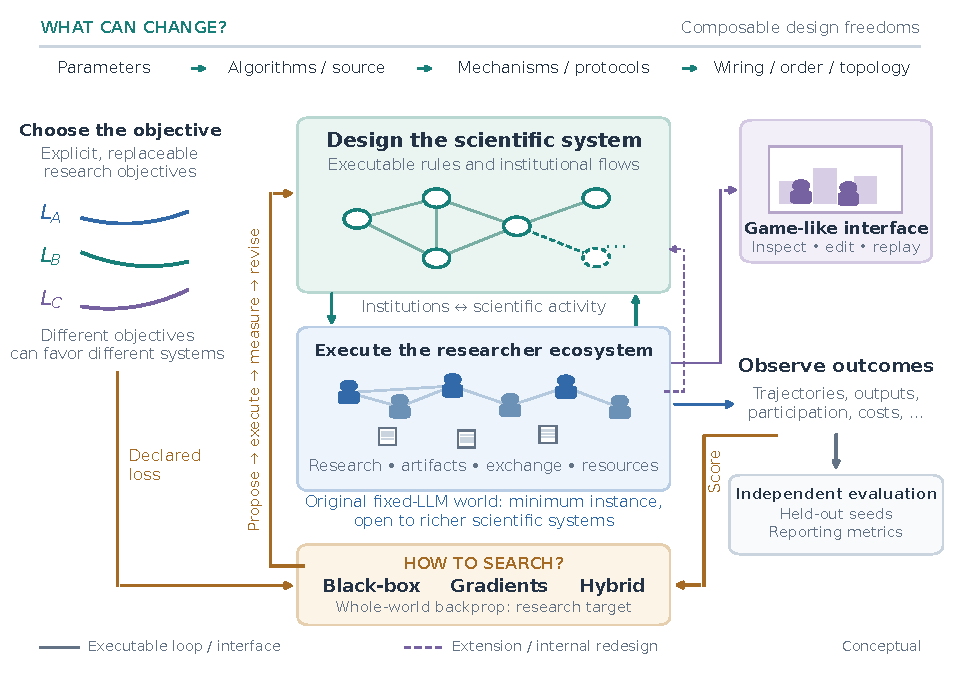
\includegraphics[width=\linewidth]{figures/program-concept/science-system-design-program.pdf}
\caption{\textbf{Research program: optimize scientific organization.}
The objective, the editable system and the search method are separate objects.
Parameters, algorithms, mechanisms and wiring/processes are design freedoms,
not four optimizer names. The native world is contained rather than replaced.
The diagram describes the research space, not proof that every experiment
uses every freedom or that any method improves scientific truth.}
\label{fig:integrated-concept}
\end{figure}

\paragraph{The research contribution and its scope.}
We present an executable formulation of scientific-system design, an integrated
native execution/search/evidence interface, and a sequence of bounded studies
that test different parts of the formulation. Parameter search demonstrates
objective-dependent selection and uncertain held-out profiles. External-author
cases establish that new source, protocols, project processes and feedback
routes can execute in the original world. Gradient studies distinguish exact
local computation, approximate response representations and conditional
expected-loss gradients. A matched local-designer study tests permitted
freedoms against stronger references without dropping failures. The game-like
interface makes the same designs and observations inspectable.

Code-defined agent search, mechanism synthesis and scientific harness
adaptation are existing research directions, not claims of priority made here
\citep{narayanaswami2022programmatic,hu2024adas,wu2026scimars}.
Our empirical target is the map from a declared objective to an executable
organizing system, its native behavioral consequences and its unused-condition
profile. Identifying that object does not yet establish a general result about
the value of free institutional design; the bounded studies below retain that
gap rather than claiming novelty for a generic propose--evaluate--revise loop.

These are not claims of a new optimization identity, a universally good
scientific institution or a trained self-improving inventor. The main empirical
tension is that \emph{representational freedom, exercised institutional change
and effective optimization are different achievements}. Wider permission
does not guarantee a submitted program; a new node need not improve loss;
a lower proxy need not improve science. The experiments make these differences
observable rather than enforce a favorable outcome.

\subsection*{Evidence at a glance: what supports which claim?}
\label{sec:evidence-at-a-glance}
The central empirical question is not whether an institution can be encoded,
or whether a chosen proxy can be made smaller than a weak starting system.
It is whether objective-conditioned search finds consequential organizing
rules beyond strong same-authority alternatives, and how those rules act in
the persistent researcher world. Table~\ref{tab:claim-evidence-map} separates
the strongest completed comparisons from claims they do not establish.
The table is a reading map, not a pooled estimate or a declaration that the
research program is publication-ready.

\begin{table}[t]
\centering\small
\setlength{\tabcolsep}{3pt}
\begin{tabular}{@{}>{\raggedright\arraybackslash}p{.20\linewidth}>{\raggedright\arraybackslash}p{.41\linewidth}>{\raggedright\arraybackslash}p{.33\linewidth}@{}}
\toprule
Completed comparison & Supported observation & Not established \\
\midrule
Matched local search (Section~\ref{sec:matched}) &
120 slots: 64 complete, 25 generation nulls, 31 execution nulls. After frozen
selection, 90 physical evaluations of 15 exact policies retain stronger rules:
throughput code, technical-only and uniform selections average 6.2 acceptances,
tying all-accept; LLM numeric retains the seed at 0.2. Review-cost code selections
average loss 1.92, worse than reviewer-free reject at 0. &
Free-design or feedback superiority; structural invention. The 90 jobs are
not 90 independent optimization histories. \\
\addlinespace
Same-authority topic rules (Section~\ref{sec:native-topic-system-search}) &
Two hand-written rules yield 20 versus 36 accepted decisions at equal
collected cost 200. Original topic durations and scientist weights are fixed;
actual topics and subsequent researcher inputs differ. &
Automatic discovery, duration-only mediation or a world-level optimum. \\
\addlinespace
Terminal resource rule (Section~\ref{sec:native-terminal-cost}) &
A hand rule improves declared resource-aware loss by 4: collected cost
200$\to$160, unpaid cost 0$\to$40, requested cost still 200. All 179 scientist
inputs/literal choices and 36 accepted records match. &
Less requested work, better science, an invented institution or long-run benefit.
The gain is retained, not disqualified. \\
\addlinespace
Source-information search (Section~\ref{sec:native-consumer-source}) &
Eight own slots retain seven completed outcomes and one native null. All four
frozen own selections tie the strong visible rule; an adverse path recovers a
supplied rule rather than a new best-known program. &
A general negative effect of source access, an impossibility of useful
institution search or a clean isolated measure of understanding. \\
\bottomrule
\end{tabular}
\caption{Evidence and inference boundaries. Losses and budgets belong to their
own studies; matching symbols do not make them a common benchmark. Hand
controls establish reachable effects but are not discoveries by the local
inventor. Technical nulls remain unavailable measurements, not bad numeric
scores. Complete programs, all attempts, costs and separate conditions remain
in the corresponding sections and appendices.}
\label{tab:claim-evidence-map}
\end{table}

\paragraph{Loss symbols are study-local, not interchangeable metrics.}
In the matched V2 study, $T=-A$ and $C=4A-Q+0.1R$: $A$ counts accepted
decisions, $Q$ sums their native peer scores and $R$ counts reviews. In the
later content/resource studies, $L_U=-U$ and $L_C=-U+0.1K$: $U$ sums centered
opinions from a fixed external abstract-content observer, while $K$ is
collected native activity cost. Native peer scores and external opinions are
different measurements; review counts and collected resource units are
different costs. Neither objective is retrospectively substituted for the
other. The historical parameter objectives and their unused-condition
evaluation remain separately defined in Section~\ref{sec:parameter}.

\paragraph{A completed finite search is not a method advantage.}
At November 16, 2026, 14:05 UTC, the later priority/free-method writer exits
normally with all 24 own observations and three references. Twelve own
observations tie and 12 worsen their visible reference; none improves it.
The 12 frozen own-only selections yield eight ties and four worse losses.
The full original paired cold/cost/readout chain is still running at the
14:11 UTC verification. Section~\ref{sec:native-priority-method-snapshot}
includes all 24 slots, while older dated receipts remain unchanged. Its author visibility/phase
defect prevents isolated attribution to objective or method; prospectively
corrected software is not an observed corrected search result. Literal
24-slot values, frozen selections and original input bindings are retained in
\path{research/results/native-priority-method-terminal-snapshot-v1.json}.

The earlier structural, gradient, nested-design and English game-interface
tracks also remain in this manuscript. Their different authors, sources and
conditions cannot be added to the matched local experiment as independent
replications. Available design freedoms and available optimizers are not
themselves evidence that those freedoms are useful or that any optimizer
improves expected institutional performance. A focused main-track claim and
adequate independent evidence remain open, even though substantial software
and finite studies are complete.

\section{Problem: objectives select organizing systems}
\label{sec:problem}
Let $S\in\Sys $ specify an organizing system, $W$ researcher-model weights, $D$
the literature corpus, $ c $ an environmental condition and $\epsilon $ residual
execution/model randomness. The native simulator generates a trajectory
\begin{equation}
 \tau\sim P(\cdot\mid S,W,D,c),\qquad m=M(\tau).
\end{equation}
It contains research directions, projects, papers, review and publication
records, resources, messages and persistent state. A declared loss $\ell_\lambda $
defines the design problem
\begin{equation}
 J_\lambda(S)=\mathbb E_{c,\epsilon}[\ell_\lambda(M(\tau))],\qquad
 \text{seek }S\text{ with small }J_\lambda(S).
 \label{eq:integrated-objective}
\end{equation}
Finite observations estimate only their declared conditions. A single saved
trajectory is neither an exact expectation nor a global optimum. Weights $W$
are fixed within each experiment, but behavior is not: a different information
route, resource state or publication history changes future LLM inputs.

\subsection{Loss, validity, evaluation and adoption}
Four contracts have different jobs (Table~\ref{tab:integrated-contracts}). The
optimized loss selects candidates. Technical validity checks whether an
observation can be obtained under the declared execution and budget contract.
Outside metrics and unused conditions characterize selected systems.
An optional adoption policy governs deployment, not the search objective.

\begin{table}[t]\centering\small
\caption{Four separate contracts. No substantive veto is implicit.}
\label{tab:integrated-contracts}
\begin{tabular}{@{}>{\raggedright\arraybackslash}p{.19\linewidth}>{\raggedright\arraybackslash}p{.49\linewidth}>{\raggedright\arraybackslash}p{.22\linewidth}@{}}
\toprule
Object & Question answered & Search role \\
\midrule
LossSpec & Which measured system is preferred under this objective? & Proposal feedback and selection \\
Validity & Did literal code execute and yield the required measurements? & Numeric loss or explicit null \\
Evaluation & What happens under other scores or unused conditions? & Withheld when declared held out \\
Adoption policy & Should a measured institution be deployed? & Separate, only if explicitly chosen \\
\bottomrule
\end{tabular}\end{table}

An execution failure has a missing loss, not an invented large penalty or a
zero score. We retain the consumed slot, draft, error and observed cost. An
objective may select a normatively unattractive institution: we do not reject
it through an undeclared fairness, novelty, participation or improvement floor.
This does not mean technical completion makes the institution desirable.
If evaluation informs the next proposal, it is development feedback rather
than held-out evidence.

\subsection{Objective design is a scientific question}
Science-of-science research motivates examining careers, knowledge production,
collaboration, diversity and institutions jointly~\citep{fortunato2018science}.
Responsible research assessment also cautions against equating a metric with
the mission it is meant to assess~\citep{hicks2015leiden}. We use this perspective
to expose objective choices, not to declare one official national-policy index
the universal target. Publication counts, topic entropy, review scores,
participation and resources can each be optimized or diagnosed; their role
must be declared before a campaign.

Optimization creates a further distinction: a useful measurement for describing
a fixed system may become a poor objective once the system can change its
measurement-generating process. A program can reduce review work by omitting
review, raise throughput by changing project timing, or select historically
favorable reviewers. Those are possible answers to a declared proxy, not
automatic evidence of epistemic progress. We therefore preserve raw components
and cross-objective profiles instead of reporting only a winner's scalar.

\section{An executable space of scientific systems}
\label{sec:design}
\subsection{Specifications, implementations and composition}
A \Spec{} declares actor/artifact types, mechanism instances, input/output ports,
directed connections, temporal latency, schedules, initial state and invariants.
A mechanism specifies an implementation and its parameters/state contract. Its
implementation can be native trusted code, isolated authored Python, an LLM
operation or a supported tensor representation. A fingerprint covers literal
specification bytes after canonical serialization; it is identity evidence,
not a measure of algorithmic novelty.

The design freedoms are related but should not be collapsed into a fixed menu:
\begin{enumerate}[leftmargin=*,nosep]
 \item \textbf{Parameters}: change settings within a fixed implementation and graph.
 \item \textbf{Algorithms}: replace executable mappings or state updates behind
 a compatible interface, not merely select a named policy.
 \item \textbf{Mechanisms}: introduce or remove actors, storage, decision services
 or source-defined institutional components with explicit consumers.
 \item \textbf{Wiring and processes}: change who receives what, when it arrives,
 the dependency order, conditional invocation and bounded repetition.
\end{enumerate}
Study-specific domains can restrict these freedoms for comparison. A valid
schema does not make every imaginable graph executable in a particular world.
For example, an empty graph may be structurally well formed but fail the
native observation contract. Omitting review requires a compatible downstream
decision consumer; the host does not invent missing reviews or silently repair
the publication rule.

Graph syntax and operational authority are different. An arbitrary program
with the same observations, state and invocation opportunities may implement
several mechanisms inside one policy. Conversely, a program invoked only
after review cannot undo the reviews already performed in that period.
Comparisons must therefore specify available observations, effects and
execution times, not only node count or the label ``free graph.'' A restricted
parameter family can lack an operation even when another code representation
could express it. Section~\ref{sec:design-diagnostics} examines these boundaries
without claiming that graph syntax is universally necessary.

\subsection{Containment of the original researcher world}
\code{NativeScienceKernel} executes specifications against the original
Simulation lifecycle. Default nodes delegate to its phase methods rather than
approximate scientist behavior numerically. A private annual frame retains
native domain objects; versioned JSON ports expose bounded records to authored
mechanisms. Review selection is separable from publication commit, so new
decision code can still affect the actual paper tracker, retrieval archive,
resource state and later researcher prompts.

Default behavior has deterministic native-lifecycle checks comparing scientific
state, RNG state and full request payloads under matching scripted replies.
These are engineering containment tests, not new Qwen experiments. The live
studies below separately use fixed local Qwen3-8B scientists and actual
literature-grounded native forwards. They are small local settings, not a
reproduction of the source paper's reported Qwen3-32B configuration.
The local four-year literature subset contains 103,107 CS records from 2016--2019,
drawn from SciEvo~\citep{jin2024scievo}. Corpus and retrieval identities are
bound separately from the researcher model; a local run is not a replication
of the source paper's model scale or full experimental population.

The extension is conservative, not unlimited. Generated code cannot import
arbitrary host objects, change researcher weights, rewrite a measurement or
invent a trusted capability by naming it. Annual native phase handlers retain
their own scientific semantics. A new kind of real activity needs an implemented
consumer, identity/accounting transport and measurement interpretation; a
record called ``discovery'' does not become a validated discovery.

\paragraph{Native effects versus a fixed historical calendar.}
The later workflow domain fixes native effect contracts rather than their
annual schedule. It permits institutional code, nodes and typed wiring while
requiring exactly-once protected effects, producers before zero-latency
consumers, opening before activity and ledger closure after mutations.
Descriptive ordering metadata is not execution authority. A structural-only
experiment can then hold sources, parameters and nodes literal and change
phases/connections alone; that experimental restriction is not the general
system language's ceiling. A hand timing control changes three phases and
five edges without rewriting any native effect. Its fresh scientist-world
loss is an empirical question, not a consequence of graph validity.
The complete new-binding software check uses seven SCRIPTED native worlds,
28 annual checkpoints, 13 bounded mock-HTTP workers and a retained generation
null, with matching double audits, costs and reports. This exercises original
production and cold readers, not real-model workflow invention or improvement.

\subsection{New institutions and their actual consumers}
Isolated Python receives declared inputs and state and returns schema-checked
outputs/state. It can implement an entirely new algorithm, generate intermediate
protocols or maintain institutional memory. It runs in a pinned, network-disabled
container, not as model-supplied code imported by the host. Output shape,
identities and required port coverage are checked; scientific merit is not.

The domain bridge supplies generic effects: persistent actor/artifact creation
and revision, namespaced state, delivery of arbitrary linked records to real
researchers, actual project-plan changes and conserving resource transfers.
Roles and schema-declared state are data; source supplies the institution's
allocation or communication rule. New actor serialization alone does not
provide autonomous behavior. Custom artifacts can link native papers but do
not increase accepted-paper counts merely by being stored.

Information must reach a consumer to matter. A message route records producer,
port, event lineage and recipient. Researcher context delivery modifies actual
LLM requests; decision outputs address real submitted papers; plan amendments
alter actual native project state. Execution receipts can establish delivery
and committed effects. Neither a node label nor the designer's explanation
establishes that the changed code ran, was read or caused a better outcome.

\subsection{Processes, time and state}
Dependencies and typed data edges define deterministic within-period ordering.
Delayed edges carry records to later periods. Controlled activities support
source-authored Boolean guards, bounded counts, persistent state and explicit
termination. Missing control can be declared a wait or an error; a skipped
activity is not fabricated research. Bounds are execution budgets, not merit
filters. Original single-shot annual handlers cannot simply be repeated with
their old IDs and side effects. Richer repetition requires repeatable activities
with genuine invocation identities and domain effects.

Checkpoints retain mechanism state, queued messages, actors, artifacts and
source binding. Resume cannot silently switch to a different institution.
This supports longitudinal feedback within a world. Most reported optimization
trials, however, reset their worlds: repeated candidate evaluation is not the
same as one society recursively redesigning itself over time.

\section{Search methods and gradient boundaries}
\label{sec:search}
\subsection{A common propose--execute--measure loop}
The persistent controller accepts a loss, initial specification, design domain,
information policy and finite budget. It saves a proposal before dispatch,
validates its literal transaction, executes a native forward, measures canonical
loss and updates eligible search history. The generic ask/tell boundary does
not require simulator derivatives. A domain adapter, not the optimizer,
understands coordinates, source replacements or graph transactions.

Black-box optimization includes uniform sampling, incumbent mutation,
local refinement and LLM proposals. The implementation supports an objective
and own-history archive, not an obligation to change or improve a candidate.
Repeated designs, worse revisions and ties consume their scheduled budget.
The host does not rewrite generated code, manufacture a terminal submission
or replace a failed slot. Trace-informed designers may inspect more than a
scalar oracle; such comparisons must disclose their richer information.

An LLM designer can emit executable definitions and structured patches. The
execution engine checks the resulting program rather than interpreting prose
as functionality. In the local matched study, the scientist and designer are
different fixed models. External-author pilots have different provenance:
they establish expressive examples and observed redesign, not local-model
invention or an authenticated independent designer identity.

\subsection{Pathwise derivatives of explicit representations}
For a supported differentiable institution $ u=f_\theta(x)$, a local backward
pass computes derivatives of that represented mapping. Tensor state and
explicit routes can carry derivatives through multiple represented operations
and invocations. Such a derivative is exact for that computation, not for an
opaque LLM, retrieval, integer parser or unrepresented native transition.

A conditional response operator $\widehat r_\phi(x,\theta)$ fitted to native
observations can supply missing response sensitivities in an approximate
path. Autograd then computes $\nabla_\theta\widehat L$, not automatically
$\nabla_\theta J$ of Eq.~\eqref{eq:integrated-objective}. Hard selection may be
relaxed by smooth probabilities while the native forward remains hard.
Temperature changes both fit and sensitivity. A low calibration error does
not establish accurate unused-condition predictions, and a useful local fit
does not make arbitrary generated source differentiable.

We keep represented derivatives, native perturbations and projected native
reevaluations separate. Opaque links remain unknown, not zero-imputed. If a
hybrid proposal combines estimates from several sources, its target, bias
and eligible data must be named; blending estimates is not an unbiasedness proof.
The native-response experiments in Section~\ref{sec:gradient-evidence} examine
this boundary directly.

\subsection{Expected-loss gradients around an opaque world}
Let a fixed generated vocabulary $V$ map explicit discrete choices and continuous
latents $ d $ to $S(V,d)$. For a declared distribution $ q_\theta(d\mid V)$,
\begin{equation}
 J_V(\theta)=\mathbb E_{d\sim q_\theta,\,\tau\sim P(\cdot\mid S(V,d))}
 [\ell(M(\tau))].
\end{equation}
Under support, integrability and differentiation conditions, and with no
additional direct $\theta $ dependence of the conditional environment,
\begin{equation}
 \nabla_\theta J_V
 =\mathbb E[(\ell-b)\nabla_\theta\log q_\theta(d\mid V)].
 \label{eq:integrated-score}
\end{equation}
This standard likelihood-ratio identity estimates a design-distribution
gradient without a world Jacobian~\citep{parmas2021unified}. It covers the
explicit categorical/Gaussian design law, not unknown probabilities of arbitrary
LLM source synthesis or researcher text. Fixed transforms from unbounded
latents to legal coordinates make the sampled density and executable value
distinct objects that must both be retained.

For $K$ IID design draws, leave-one-out baselines exclude the scored draw's
own loss. For a prior-frozen surrogate $ c(d)$ with tractable expectation,
\begin{equation}
 \nabla_\theta J_V
 =\mathbb E[(\ell-c(d))\nabla_\theta\log q_\theta(d\mid V)]
  +\nabla_\theta\mathbb E_{q_\theta}[c(d)].
 \label{eq:integrated-control}
\end{equation}
The correction matters; inaccurate controls need not bias this identity but
can increase variance. Fitting on the current scored batch or omitting the
correction changes its justification. Composable gradient frameworks and
composite estimators motivate these interfaces, not a claim to have reproduced
their complete algorithms~\citep{parmas2022proppo,parmas2023composite}.

Validity-dependent missing losses need special care: discarding failed draws
does not automatically estimate the unconditional expectation above. We keep
null batches and unavailable updates explicit. A campaign may instead declare
a failure-valued estimand in advance, but these studies do not invent one after
observing failures. A computed update and a distribution actually evaluated
after that update are also separate evidence.

\subsection{Changing the design language itself}
An outer author can use its own measured history to change $V$: new source,
mechanisms, factors, coordinate meanings and wiring. Inner score updates stay
conditional on the current $V$. If an outer revision removes a coordinate or
changes its meaning, old gradients/control state are not silently transported.
A point-mass design or retaining the incumbent is legal. Section~\ref{sec:nested}
executes this outer-design/inner-update composition in the original world.
It is an application of existing search and estimation ideas, not a new
theory of differentiable program synthesis.

\subsection{What finite searches and fixed-policy comparisons estimate}
\label{sec:finite-estimands}
Let $\mathcal C_{\lambda mh}$ be the declared eligible candidate pool for
objective $\lambda$, proposal method $m$ and design history $h$. Eligibility
here means the protocol's selection pool, not a hidden scientific-merit test.
Write $\mathcal V_{\lambda mh}\subseteq\mathcal C_{\lambda mh}$ for the
complete eligible designs. After development, retain the entire observed minimum set
\begin{equation}
 \mathcal B_{\lambda mh}=
 \mathop{\mathrm{arg\,min}}_{S\in\mathcal V_{\lambda mh}}
 \widehat L^{\mathrm{dev}}_\lambda(S),
 \label{eq:finite-minimum-set}
\end{equation}
and apply only the predeclared tie rule to choose an evaluation specification
$S^*_{\lambda mh}$. Equal losses do not establish equivalent programs or
identical trajectories. An initial/reference policy belongs to the pool only
when that protocol makes it eligible; submitting an unchanged reference is
legal but is not new invention. An empty eligible complete pool leaves an
unavailable selection, not an automatically substituted baseline.

For a fixed selected policy and an explicit reference $S_0$, the common-condition
comparison is
\begin{equation}
 \Delta_{\lambda mh}(c)=
 L_\lambda(S^*_{\lambda mh};c)-L_\lambda(S_0;c).
 \label{eq:reference-relative-loss}
\end{equation}
Negative values favor the selected policy under that same objective. Different
losses need not have comparable units, so comparing the magnitudes of T and U
is not a method ranking. A common world seed names a matched environmental
condition, not identical residual LLM randomness after two policies generate
different requests. Pairing is therefore by declared condition and actual
observations, not by an assumption that every stochastic event is shared.

Variation over unused $c$ characterizes the already selected policy. Variation
over independently repeated $h$ is also needed for an expected claim about the
search procedure that selects it. More evaluation seeds for one selected
specification do not become more independent optimization histories. Pooling
several development histories into one winner likewise yields one selected
policy per arm, not one held-out result per history. Different source snapshots,
design domains, horizons and observers below are not pooled into a method
effect.

A technical null in either member makes that pair's loss difference unavailable.
All attempted, failed and unattempted slots remain visible with their actual
costs. Reporting loss only for completed pairs is conditional evidence and
must accompany coverage; it is not an unconditional end-to-end risk estimate.
No retrospective failure penalty is introduced to obtain a numerical ranking.
Cross-objective scores reuse a trajectory's measurements when available;
they are not additional world samples. Cached judgments of identical content
similarly remain the same physical opinions, not independent replications.

The objective-to-system question includes both its selected outcomes and its
path: literal revisions, exercised effects, native consequences and cost.
Different objectives may return overlapping minimum sets. If the objective
also changes a loss-selected editing parent, the contrast concerns the entire
objective-conditioned search, not scalar feedback alone with the parent held
fixed. None of these definitions requires different winners or a positive gain.
\FloatBarrier

\section{Evidence strategy: complementary studies, not pooled replication}
The research questions require different tests. A fixed-topology study isolates
objective-conditioned parameter selection. Structural cases test whether novel
source, protocols and routes actually reach native activities. Gradient pilots
test derivative meaning and subsequent native forwards. The latest matched
study compares local-designer packages and stronger references on a common
source. Table~\ref{tab:integrated-studies} summarizes these roles.

\begin{table}[t]\centering\small
\caption{Evidence families retained in the integrated argument. Counts are
within-study budgets, not additive independent replications. Historical
source/model/feedback differences prevent pooling method rankings.}
\label{tab:integrated-studies}
\begin{tabular}{@{}>{\raggedright\arraybackslash}p{.19\linewidth}>{\raggedright\arraybackslash}p{.21\linewidth}>{\raggedright\arraybackslash}p{.25\linewidth}>{\raggedright\arraybackslash}p{.25\linewidth}@{}}
\toprule
Family & Design/author & Native evidence & Question addressed \\
\midrule
Parameter study & Eight fixed-topology settings; adaptive random search & 45 logical development rows; 15 sealed evaluation runs & Can objective changes select different systems and profiles? \\
Structural cases V8/V12 & External source/protocol/graph author & Eight/six two-year worlds & Do new mechanisms, routes and plan processes execute? \\
Nested case V13 & External vocabulary + conditional LR + redesign & Eight worlds; 592 fresh replies & Can inner updates and outer source changes share a native loop? \\
Gradient cases V9--V11 & Response representation, local refinement, score/control estimator & Coupled paths and eight reset worlds, separately bound & Does backward mean fidelity, a native-tested update or superiority? \\
Matched study V2 & Local 35B designer and uniform numeric control & 120 attempts; 90 selection-fixed evaluations & What is achieved under matched permitted freedoms and stronger references? \\
\bottomrule
\end{tabular}\end{table}

Across native case studies, five original researchers and fixed Qwen3-8B
weights retain language decisions, literature grounding, projects and papers.
Most cases use two years and development seed 42; the older parameter study
uses four-year worlds and a different source/seeding protocol. A common seed
does not force equal fresh LLM realizations. We distinguish reset worlds,
common-prefix-coupled forwards, conditional IID design draws and genuinely
unused evaluation conditions. No new inference is introduced by this synthesis.

\section{Objective-conditioned parameter optimization}
\label{sec:parameter}
\subsection{Design and sealed evaluation}
The first study varies eight institutional settings within one fixed topology:
acceptance rate, funding application cost, funding slot fraction, resubmission
cost, review policy, reviewer capacity, reviewer matching and reviews per paper.
The simulator, adaptive-random-search rule, five-candidate budget and development
seeds 601/607/617 are held fixed while the optimized LossSpec changes.
For valid run $ r $, the losses are
\begin{align}
 \ell_r^{\rm part}&=1-a_r+0.05b_r,&
 \ell_r^{\rm topic}&=-h_r,&
 \ell_r^{\rm burden}&=b_r,
\end{align}
where $ a_r $ is active-researcher fraction, $ b_r $ review burden per active
researcher and $ h_r $ topic entropy. Each arm minimizes the development mean
plus $0.25$ population standard deviations over its three seeds. Entropy is
not truth, and burden can fall by suppressing evaluation. These deliberately
narrow proxies stress the objective-to-system map.

All 45 logical design--seed rows terminate: 30 complete and 15 fail at the declared
reviewer-capacity boundary, retaining null loss. Twenty-nine development rows
are physically executed and 16 logical rows adopt byte-identical initial
trajectories under the study's provenance contract. Thus 45 logical rows are
not 45 fresh native worlds. All winners are sealed before a common evaluation
on unused seeds 701/709/719/727/733; all 15 arm-labelled runs complete.

\subsection{Different objectives, two actual designs}
Participation/review selects proposal 2 with development loss 0.321846. Topic
and burden select proposal 1, with losses $-1.696931$ and $1.668963$. In the
topic arm proposals 1/2 tie, so the predeclared earliest rule selects 1. Only
participation has multiple valid adaptive proposals beyond the initial pair;
later topic/burden proposals fail technical validity. The paths show an
executable own-observation loop, not rich or repeatable path divergence.

The selected participation design has acceptance rate 0.4968, capacity 8,
topic-based matching and three reviews per paper. Topic/burden share a design
with rate 0.1132, capacity 2, random matching and four reviews per paper.
Three objective labels therefore produce two designs, not three institutions.
Full settings appear in Appendix~\ref{app:parameter}.

\begin{figure}[t]\centering
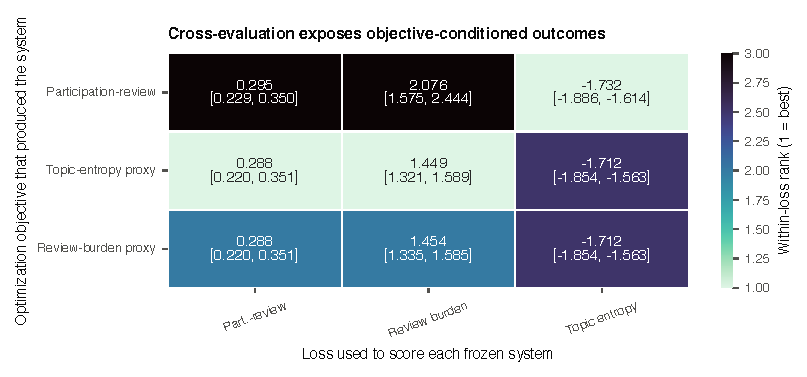
\includegraphics[width=\linewidth]{generated/metric-conditioned/figures/metric-conditioned-cross-evaluation.pdf}
\caption{\textbf{Historical parameter study: sealed-system cross-evaluation.}
Numbers are each complete LossSpec aggregate with the study's exact-bootstrap
percentile intervals over five unused seeds; color ranks within a loss only.
Topic and burden rows encode the same design but separate stochastic evaluations.
All nine paired-contrast intervals include zero. Descriptive ordering is not
stable superiority or evidence that every objective discovers a distinct system.}
\label{fig:integrated-parameter}
\end{figure}

On unused conditions, the participation-selected design has aggregate losses
0.295 on participation, 2.076 on burden and $-1.732$ on topic. The duplicated
topic/burden design has approximately 0.288, 1.449--1.454 and $-1.712$.
Ordering changes with the scoring loss, but every one of the nine paired
95\% intervals includes zero. The apparent rank reversal is descriptive.
The selected design is not necessarily best under its own unused-condition loss.

Operational differences are clearer than normative conclusions. The
participation-selected design averages 11.6 accepted papers and full review
coverage, versus 4.0 and approximately 0.55 for the other design. It also has
higher burden, approximately 1.959 versus 1.415--1.421. Activity fractions 0.82
versus 0.80 and topic entropies 1.771 versus 1.750 remain uncertain at five seeds.
This is not a welfare ranking, optimizer comparison or structural-search result.

\section{Executing institutions beyond fixed parameter menus}
\label{sec:structural}
\subsection{A new planning and delayed-feedback route}
The external-author V8 case permits source, intermediate protocols, node
addition/removal, wiring and activity processes. Two objectives use
$T=-A$ and $U=3.25A-Q+0.05R$, where $A$ counts accepted native decisions,
$Q$ sums original reviewer-score means on accepted decisions, and $R$ counts
review records. Authored final scores do not create $Q$. Each objective has
two generations and two conditional-IID draws per generation.

All eight native worlds complete with 734 fresh Qwen replies. The developer
seed has 19 nodes/27 edges; evaluated graphs have 16--18 nodes/22--24 edges.
Throughput losses are $[-9,-9,-10,-10]$; utility losses are
$[0, 0, 0.4833, 0.4833]$. All outcomes are retained in
Appendix~\ref{app:structural}; these same-seed development worlds are not
an unused-condition causal comparison.

Throughput redesign replaces hash-selected plan eligibility with actual
deadline inspection and annual amendments. In the first revised world,
a researcher whose project would finish in year 2 has a real amended plan
finishing in year 1 and an actual year 1 accepted-paper record. Five rather
than four year 1 submissions/acceptances are recorded. A newly wired publication
receipt route delivers earlier paper identities to the year 2 planning node,
and resulting focus text reaches actual researcher requests.

Timing limits the mechanism claim. The extra year 1 acceptance occurs before
any prior publication receipt exists; it cannot be attributed to that delayed
feedback. Source, scope, focus and wiring change jointly, without component
ablation. What is established is an exercised plan/record/information path,
not the independent benefit of the added feedback loop.

The utility revision adds review-digest feedback and restores review. It accepts
one paper with mean score $11/3$ after 18 reviews, yielding
$3.25-11/3+0.05(18)=0.4833$. The initial no-review/no-acceptance observations
remain better at 0. A new mechanism can be technically real and worse under the
declared objective. No quality or participation veto reverses that result.

\subsection{An executed new mechanism that is not retained}
The V12 case gives each objective three own-history source redesigns. All six
worlds complete with 565 fresh replies. Throughput installs a production office,
annual scheduler and all-accept decision source, producing 10 native plan
amendments and 10 acceptances per world. Later generations retain the exact
first institution; the loss path $[-10,-10,-10]$ is not repeated invention.

Utility begins with an evidence office and an original-review threshold above
3.25. Its G1 introduces a genuinely executed milestone-clinic node, typed
amendment transport and two wires, and changes evidence-topic matching. It
shortens one project and extends another to a two-year cycle; it is not simply
a universal acceleration rule. The native world completes, but utility worsens
from $-1/6$ to 0 with 15 reviews. G2 returns to the G0 incumbent, giving
$[-1/6, 0,-1/6]$.

The G2 parent is the best G0, not chronological G1. A zero parent diff therefore
correctly records retention, while the chronology still exposes the unsuccessful
clinic. This case matters because it demonstrates actual mechanism/wiring
freedom without selecting only successful-looking revisions. It does not
establish which simultaneous edit caused the changed loss.

\section{Nested free design and conditional distribution updating}
\label{sec:nested}
\subsection{One loop, two levels of freedom}
The V13 case combines an externally authored institutional vocabulary with
one within-vocabulary likelihood-ratio update and a fresh native followup.
Each of two losses, $T=-A$ and $E=-Q+0.5R$, receives exactly four scheduled
worlds: two IID G0 design draws, one draw from saved updated G0 weights and
one free G1 source redesign. All eight complete with 592 fresh scientist replies
and no response reuse. Every world resets development seed 42. The external
Codex author identity is self-reported, not authenticated local-Qwen authorship.

For two draws, the implemented LOO estimate is
\begin{equation}
 \widehat g=\tfrac 12\left[(L_0-L_1)s_0+(L_1-L_0)s_1\right],\qquad
 s_i=\nabla_\theta\log q_\theta(d_i\mid V),\quad
 \theta^+=\theta-0.1\widehat g.
\end{equation}
The followup uses exactly that saved vocabulary/distribution and performs no
extra update. G1 then sees only its own three preceding observations, source,
failures and saved update; it may change algorithms or support. Removing all
coordinates explicitly creates a point mass rather than silently reusing old
weights. A completed update is not itself evidence of lower expected loss.

\begin{table}[t]\centering\small
\caption{\textbf{All nested-study outcomes.} These are same-development-seed
worlds, not independent scientific seeds. $Q$ is original peer evidence.
The post-update draw is not omitted when it worsens.}
\label{tab:integrated-nested}
\begin{tabular}{llrrrrr}\toprule
Optimized loss & Stage & $A$ & $Q$ & $R$ & $T$ & $E$\\\midrule
Throughput & G0 draw 1 &7&0&0&-7&0\\
 & G0 draw 2 &7&0&0&-7&0\\
 & Updated G0 &6&0&0&-6&0\\
 & Free G1 &10&0&0&-10&0\\\addlinespace
Reviewed production & G0 draw 1 &6&20&6&-6&-17\\
 & G0 draw 2 &6&18.5&12&-6&-12.5\\
 & Updated G0 &6&12&4&-6&-10\\
 & Free G1 &6&21&6&-6&-18\\\bottomrule
\end{tabular}\end{table}

\subsection{Distribution changes and native-tested redesign}
Equal initial throughput losses give zero centered advantages and unchanged
Gaussian mean. Its next native draw has loss $-6$, worse than $-7$; it is not
reported as a successful gradient proposal. Reviewed-production losses
$[-17,-12.5]$ produce a nonzero update: the coverage latent mean changes from
1.5 to 1.671086 and reviewer-count logits from $(-1, 1,-1)$ to
$(-1, 1.225,-1.225)$. The next native draw has loss $-10$, also worse than its
prior best. Neither sample demonstrates expected improvement or estimator
superiority, nor does one worsening sample refute the score identity.

The later throughput source revision replaces mixed-cycle hashing with
universal annual scheduling while preserving native topic, focus and reason
fields. The zero-review dispatcher and compatible all-accept rule remain.
Observed loss improves from $-7$ to $-10$. Reviewed-production G1 replaces the
coverage lottery with full coverage and one eligible reviewer per paper, ranked
by its own historical scores. A read-only join rechecks the 22 original review
records used in that ranking, including shrinkage toward a pooled mean.
Task identities change, but actual Qwen reviews and the original parser still
determine $Q$. Its observed loss improves from $-17$ to $-18$.

\begin{figure}[p]\centering
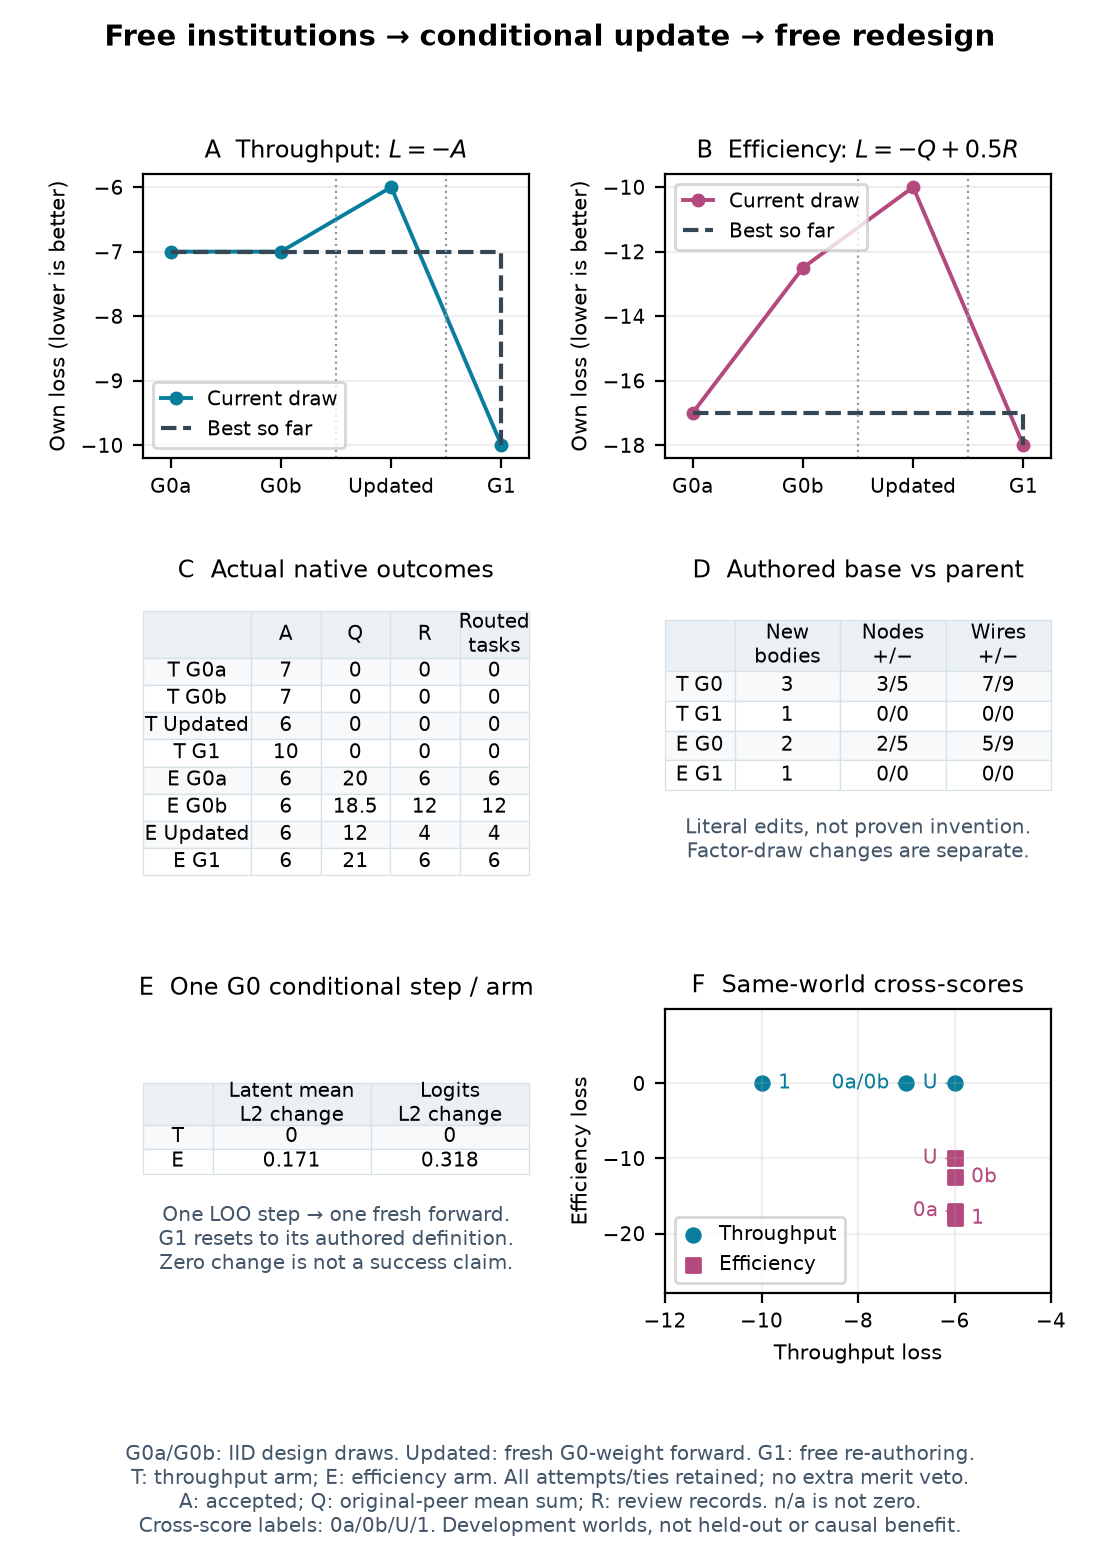
\includegraphics[width=\linewidth,height=.79\textheight,keepaspectratio]{figures/native-nested-search-v13-a1.png}
\caption{\textbf{Complete native nested-design paths.} Current observations,
best-so-far, actual $A/Q/R$, literal changes and conditional updates remain
separate. Both gradient followups are worse than their prior best; both later
external code revisions improve their observed first best. ``Efficiency'' here
means the illustrative $E$ proxy, not scientific efficiency or welfare.
Cross-scores reuse the same checkpoints; they are not held-out evidence.}
\label{fig:integrated-nested}
\end{figure}

Initial free vocabularies already differ from their common parent; G1 changes
one source body in each arm while graph sizes remain 17/25 and 16/23. Thus these
are algorithmic edits without new G1 topology. Actual source/plan/wire/task
receipts verify 40 source executions, 16 complete-plan effects, 16 routing events
and 28 review records. These establish exercised native effects, not a causal
decomposition of the gain. Favorable-reviewer selection exposes a proxy-seeking
route, not improved scientific evaluation. No hidden merit veto removes it.

\section{What native gradient experiments establish}
\label{sec:gradient-evidence}
\subsection{A fitted response representation can fail unused conditions}
The V9 case varies a charter's evidence weight $\theta $, paired with originality
weight $1-\theta $. The charter enters actual year 2 reviewer requests after the
pre-intervention native history. Scientist weights and the original integer
review parser stay fixed. The loss is $U=3.25A-Q+0.05R$.

Three calibration endpoints $\theta=(0.2, 0.5, 0.8)$ fit per-review raw-response
operators. Calibration-loss RMSE chooses a declared relaxation temperature;
the operator and proposal are frozen before unused coordinates 0.35/0.65 are
read. At the center, a clipped negative-gradient step is followed by a native
execution, even if it is a no-op. These are unused coordinates within one
development history, not unused world seeds.

Six forwards use a verified 53-reply common prefix and then 31 fresh replies each:
504 logical responses comprise 318 replays and 186 new calls. They are not six
independent societies. The fitted temperature 0.01 achieves calibration-loss
RMSE$1.16\times 10^{-5}$, yet its center derivative is only
$1.15\times 10^{-15}$. The prescribed proposal is the unchanged 0.5, with native
loss 0.9. The known lower calibration endpoint at 0.8 is not substituted for it.

At unused 0.65, predicted loss is approximately 0.8168 but native loss is 0.9.
Across $0.35\to 0.65$, native change is zero, the response-aware representation
predicts $-0.08395$, and the frozen-response baseline predicts zero. The
representation therefore fails the declared finite-path check and does not
improve prediction here. This is a substantive boundary result: native
ingress, identity joins, loss accounting and backward all execute, while
fidelity and a useful native update remain unestablished.

\subsection{Different update paths, the same observed incumbent}
V10 compares represented gradients with local derivative-free interval
refinement, charging both three shared historical calibration evaluations
and three fresh attempts. The current coordinate starts at 0.5, but both already
know the historical incumbent 0.8 with loss $49/60\approx 0.8167$.
The gradient method has raw responses/traces; the black-box method receives
coordinates/scalars only. Equal evaluation count is not equal information.

\begin{table}[t]\centering\small
\caption{Native-tested moving paths. Both methods know the better historical
point before these proposals. A moving current iterate is not a new best.}
\label{tab:integrated-method-paths}
\begin{tabular}{lrrrr}\toprule
Method & $\theta_1$ & $\theta_2$ & $\theta_3$ & Native loss sequence\\\midrule
Represented gradient & .6000 & .6488 & .7488 & $(.9000,.8167,.8167)$\\
Black-box refinement & .6500 & .7250 & .7625 & $(.9000,.8167,.8167)$\\\bottomrule
\end{tabular}\end{table}

All six fresh attempts complete, generating 186 new replies after their shared
prefixes. The represented derivatives $(-.24092,-.09762,-1.24626)$ yield different
coordinates, but native loss sequences coincide and neither beats the already
known incumbent. This demonstrates real proposed updates and measured paths,
not a gradient advantage. Appendix~\ref{app:gradient} retains the temperature
diagnosis explaining why calibration fit alone was insufficient.

\subsection{Conditional LR and corrected controls reach native execution}
V11 uses explicit mean/minimum reviewer aggregation and a bounded cutoff
driven by a Gaussian latent in one authored vocabulary. Eight fresh worlds
compare a derivative-free feedback heuristic with score updating. Both arms
observe $[0.7833333, 1.2, 1.2, 1.2]$ and retain their first incumbent; 742 fresh
replies are recorded. Prior-frozen controls implement
Eq.~\eqref{eq:integrated-control}, but the final control update is saved after
the last measured batch, not tested again within that budget.

A separately budgeted two-world V12 followup evaluates that exact saved
distribution: minimum aggregation at cutoff 3.549508 gives $A=Q=0,R=21,U=1.05$;
mean aggregation at 3.080488 gives $A=2,Q=7,R=21,U=0.55$. These 180 fresh replies
close the missing-forward question. The two outcomes do not establish lower
expected loss, lower variance or a concurrent advantage over V11's historical
outcomes. The distinction between a computed derivative, a saved proposal
and a native-tested distribution is preserved across all these cases.
\FloatBarrier

\section{Matched local-designer comparison with stronger references}
\label{sec:matched}
The preceding cases establish executable freedoms and bounded observations,
but differ in source, author and feedback. They cannot answer whether a local
code/graph designer outperforms parameter tuning. V2 therefore fixes one native
source and compares proposal packages prospectively. It is complementary
evidence, not a replacement for the earlier structural and gradient questions.

\subsection{Objectives, domains and information boundaries}
The study uses five researchers, fixed Qwen3-8B scientist weights, a four-year
CS literature corpus, two-year development worlds and common world seed 42.
The primary minimized losses are
\begin{equation}
 T=-A,\qquad C=4A-Q+0.1R.
\end{equation}
The earlier $E=-Q+0.5R$ is diagnostic only, not a third search arm. The older
$U=3.25A-Q+0.05R$ remains a different study's objective. No coefficient is
retuned from V2 results. The common editable seed is not the untouched legacy
institution; both are evaluated separately.

Each primary objective has five proposal policies:
\begin{enumerate}[leftmargin=*,nosep]
 \item LLM numeric: six declared coordinates, fixed source and topology.
 \item LLM code/fixed graph: those coordinates and three existing Python bodies.
 \item LLM code/graph: any valid specification within the native study contract.
 \item Technical-only code/graph: the same broad domain without scientific-loss
 feedback, using the fixed initial parent and its own technical history.
 \item Uniform numeric: independent samples of the same six coordinates, without
 a designer-model call.
\end{enumerate}
The six coordinates are two existing tensor thresholds, bias, memory cost,
router threshold and integer process count. Domains are checked against the
initial anchor, not the previous parent, so gradual edits cannot escape a
restricted arm. The code/graph domain permits structure change but cannot
change scientist weights, corpus or measurement functions.

All LLM arms use the same approved local 35B designer profile: 16 charged actions,
8192 output tokens, 40960 context, temperature 0.6, thinking off, 10s connect/900s
read allowances, without hidden transport retry or slot refill. Technical
errors expose the same exception-class channel. Three fresh controller
histories, each four generations per arm, give 120 candidate slots. Controller
seeds 42/1031/2063 are not independent development worlds: every forward still
uses world seed 42. Reference results and other arms' histories are not supplied
to the designer. Fresh source/model/backend-bound interface controls precede
dispatch; exact-copy equality is diagnostic, not a merit criterion.

Technical-only filtering hides losses, measurements, loss-selected parents,
incumbent indicators and derived outcome metadata, not merely the scalar text.
The intervention therefore includes parent selection, not only score display.
Technical success remains visible and may itself be informative. This is a
bounded information policy, not an adversarial isolation theorem about the
entire operating environment.

\subsection{References, selection and unused conditions}
Nine fresh references share the same source/world: legacy, editable seed,
rank/rate, all-accept, all-reject, score thresholds 3/4 and reviewer-free
accept/reject. Earlier S1 controls are not reused as these fresh observations.
These references prevent attributing a weak-seed improvement to successful
invention when an obvious rule already achieves it.

After all search slots, each objective/arm chooses from every completed
candidate plus the initial system using only its declared loss. Every exact
tie is retained; the earliest declared chronology supplies the representative.
An initial selection is reported as no discovered improvement, not a generated
replacement for failed proposals. The selection manifest is frozen before
unused-condition evaluation and its results never return to search.

The 19 logical labels comprise 15 exact policies. Explicit sharing gives 90
physical jobs: each policy on five unused seeds 31001/31013/31019/31033/31039
for two years, plus a separate four-year diagnostic at 31001. Shared labels
do not create independent samples; four years is not pooled with the five
two-year observations. All 90 jobs finish normally.

\subsection{All attempts, paths and exercised freedoms}
% Generated from CLOSED report 75f64370d673699553f69c480c93b90c07c2babba70b4f924cbc54438ab9d732
\begin{table}[t]
\centering\small
\begin{tabular}{@{}llrrrrrr@{}}
\toprule
Obj. & Proposal space/control & Meas. & G-null & X-null & M-null & Best & Ties\\
\midrule
$T$ & LLM numeric & 0/12 & 12 & 0 & 0 & 0.000$^{\ast}$ & 1\\
$T$ & LLM code, fixed graph & 9/12 & 1 & 2 & 0 & -7.000 & 9\\
$T$ & LLM code and graph & 7/12 & 0 & 5 & 0 & -7.000 & 6\\
$T$ & Technical-only code/graph & 7/12 & 0 & 5 & 0 & -7.000 & 5\\
$T$ & Uniform numeric & 12/12 & 0 & 0 & 0 & -7.000 & 8\\
\midrule
$C$ & LLM numeric & 0/12 & 12 & 0 & 0 & 2.400$^{\ast}$ & 1\\
$C$ & LLM code, fixed graph & 6/12 & 0 & 6 & 0 & 2.100 & 2\\
$C$ & LLM code and graph & 8/12 & 0 & 4 & 0 & 2.100 & 2\\
$C$ & Technical-only code/graph & 3/12 & 0 & 9 & 0 & 2.400$^{\ast}$ & 3\\
$C$ & Uniform numeric & 12/12 & 0 & 0 & 0 & 2.400$^{\ast}$ & 4\\
\bottomrule
\end{tabular}
\caption{\textbf{All scheduled development attempts.} Each row pools three
controller histories with four proposals each, all at world seed~42.
Meas.: available assigned losses; G/X-null: generation/execution failures;
M-null: completed forward with unavailable assigned loss. Nulls are not penalties.
Best includes the shared initial system; $\ast$ marks its selection, not an invention.
Ties count all exact minimizers, including the initial reference when tied.
Only display values are rounded; selection uses unrounded report values.
Controller histories are not independent environment replications.
}
\label{tab:v2-search-outcomes}
\end{table}

Of 120 slots, 64 complete, 25 fail generation and 31 fail execution.
All 24 uniform numeric proposals execute; all 24 LLM numeric proposals exhaust
their action budget without a valid explicit submission. One fixed-graph code
proposal also fails generation. The technical nulls are not numeric bad losses.

A bounded inspection confirms the correct six-coordinate contract in all 24
initial numeric-arm HTTP requests, with initial prompt counts 12145--12411,
40960 context and 8192 output settings without truncation. The general editor
protocol and restricted session domain coexist. This refutes the narrow claim
that the contract was absent; it does not establish clear salience, comprehension,
later-call capacity or the cause of every failure. The end-to-end comparison
therefore includes interface compliance and does not isolate intrinsic
expressivity. Literal error categories appear in Appendix~\ref{app:failures}.

Full-spec inspection joins all 64 complete candidates and all frozen ties.
Forty candidates change selection source, and others change existing numeric
settings. None changes declared node IDs/order, wiring, node ABI, initial state
or schedules. Twenty change numeric process count, so unchanged graph metadata
is not proof of unchanged runtime behavior. The code/graph label denotes
permission, not a structural invention observed in this study.

\begin{figure}[p]\centering
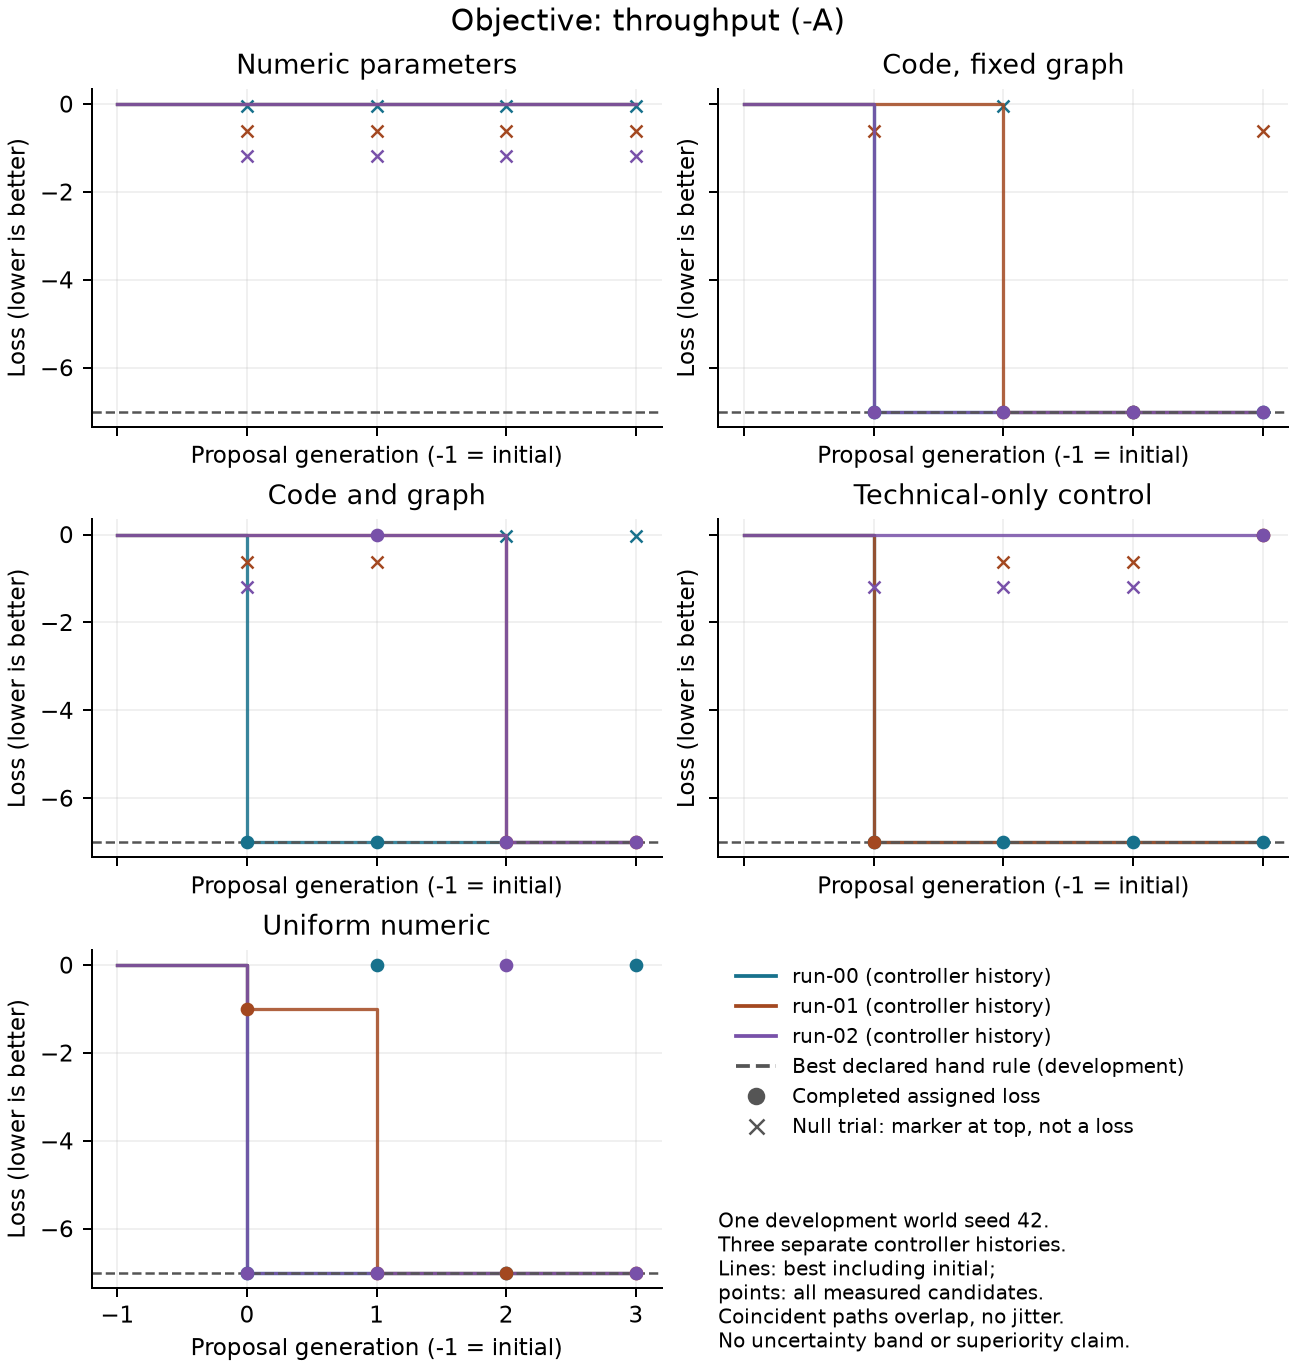
\includegraphics[width=\linewidth,height=.80\textheight,keepaspectratio]{figures/native-design-v2/throughput-paths.png}
\caption{\textbf{All V2 throughput histories.} Every measured candidate and
generation/runtime null remains. Lines show best including the shared initial
observation; a line through a null does not make that attempt successful.
The hand-rule line is a stronger reference, not an extra objective or veto.
Three controller histories use the same development world seed.}
\label{fig:integrated-v2-t}
\end{figure}
\begin{figure}[p]\centering
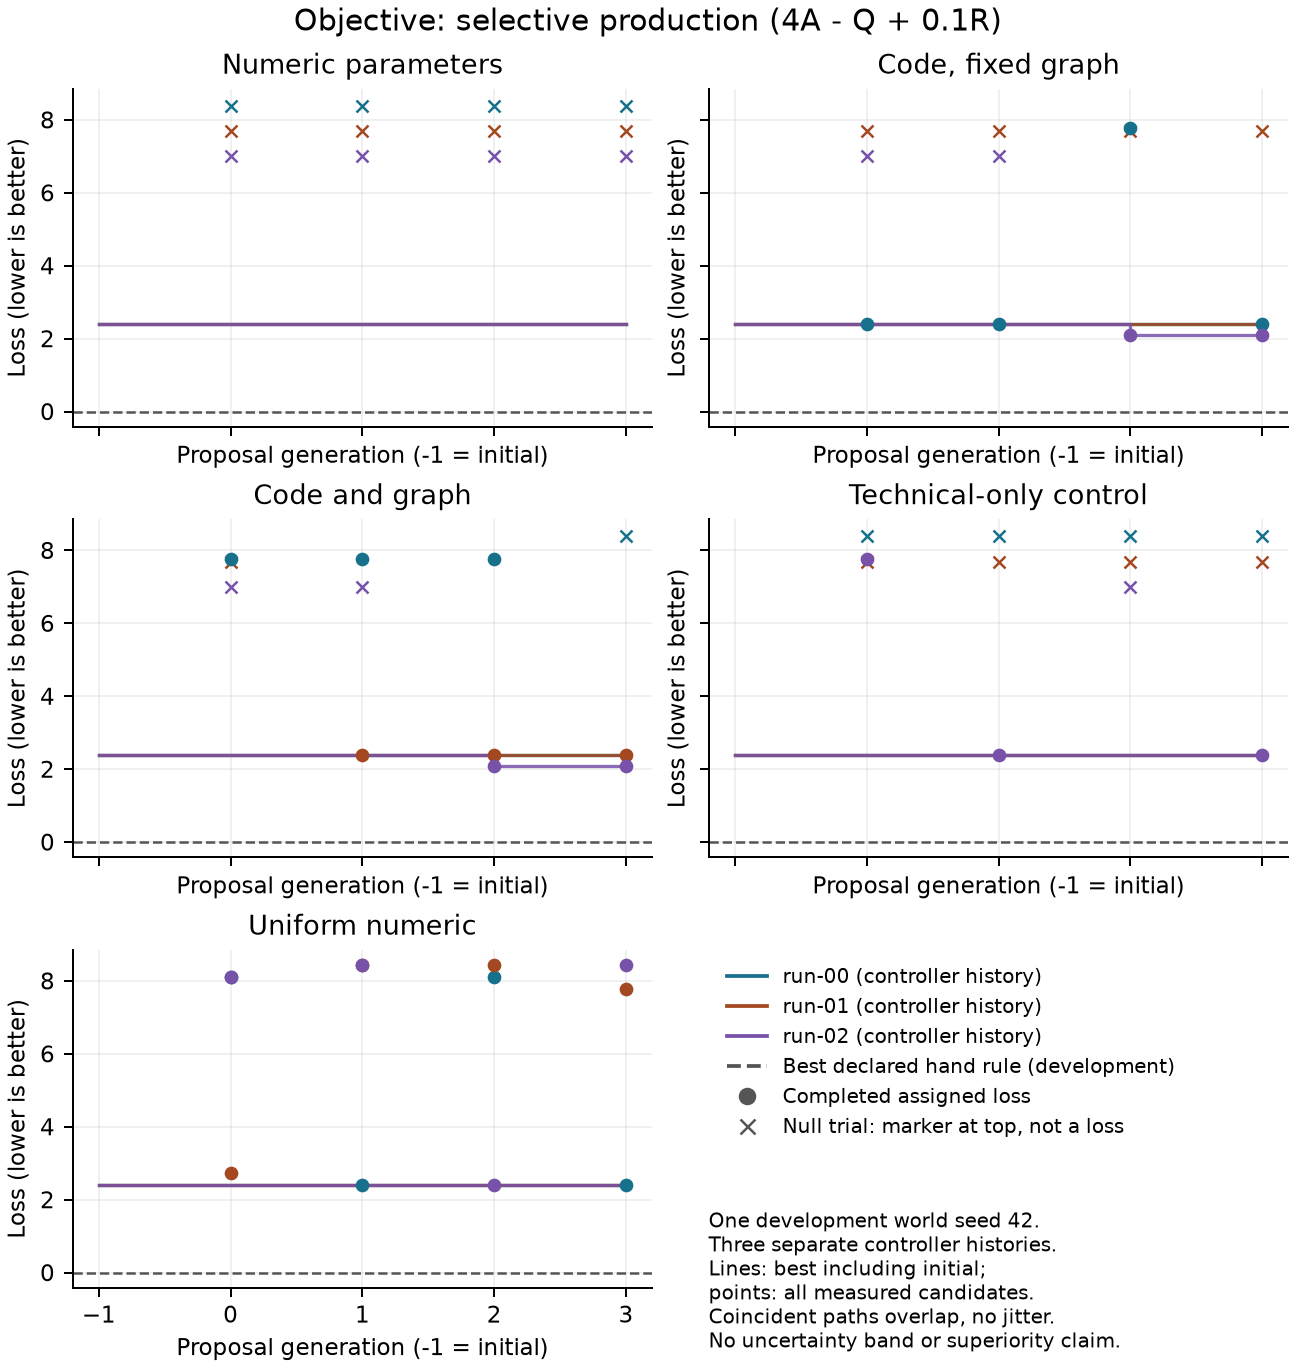
\includegraphics[width=\linewidth,height=.80\textheight,keepaspectratio]{figures/native-design-v2/selective-paths.png}
\caption{\textbf{All V2 review-cost-sensitive histories.} Code minima improve
editable initial 2.4 to 2.1, but not reviewer-free reject 0. Uniform and technical-only
controls are retained even when they tie or do not improve. Own-loss units are
not comparable to the throughput panel's units.}
\label{fig:integrated-v2-c}
\end{figure}

Throughput repeatedly reaches $T=-7$, matching all-accept at development seed 42.
Uniform numeric and technical-only proposals also reach it. For $C$, code
minima 2.1 improve editable initial 2.4 but not reviewer-free reject 0.
Initial policies are selected for both LLM numeric arms and for $C$ technical-only
and uniform arms. The whole path, rather than its most favorable history,
provides no evidence of feedback or free-design superiority.

\subsection{Selected policies under common evaluation scores}
Figure~\ref{fig:integrated-v2-cross} reports every reference and selected label
under common $T/C/E$. Executable throughput code/control and uniform selections
average 6.2 acceptances over five unused two-year seeds, matching all-accept
and score 3. Legacy averages 2.6 and the editable seed 0.2. Reviewer-free
accept-all also averages 6.2, with $Q=R=0$: equal throughput is not equal
review-backed production or better science.

Both $C$ code selections have mean $A=Q=0,R=19.2$, hence mean $C=1.92$.
Editable seed and review-based reject-all each average 2.58; reviewer-free
reject remains 0. Diagnostic mean $E=9.6$ is not favorable reviewed production.
The different objective selects different observed acceptance/review behavior,
but these data do not identify a novel optimal policy.

\begin{figure}[p]\centering
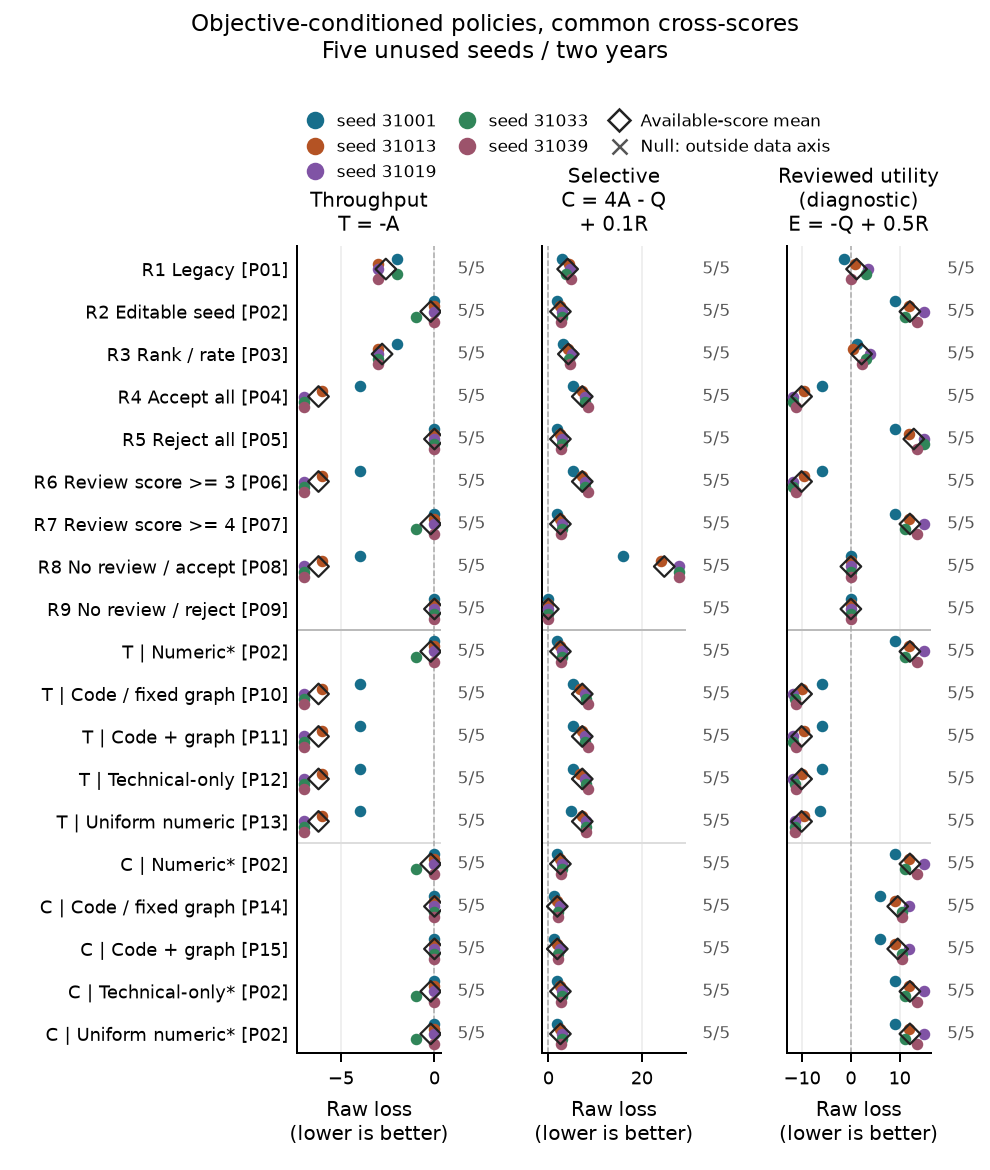
\includegraphics[width=\linewidth,height=.80\textheight,keepaspectratio]{figures/native-design-v2/cross-objective-2y.png}
\caption{\textbf{All selection-fixed V2 policies on five unused two-year seeds.}
Points are raw world observations; hollow diamonds are descriptive means, not
confidence intervals. Separate loss scales are neither normalized nor averaged.
P labels mark exact policy/job sharing, and stars mark initial selections.
E is diagnostic, not an E-optimized experiment.}
\label{fig:integrated-v2-cross}
\end{figure}

At the separate four-year seed, throughput executable selections and all-accept
each produce 11 acceptances. Both $C$ code selections have $A=Q=0,R=33$,
giving $C=3.3$, versus initial 6.9 and reviewer-free reject 0. Some equal-throughput
policies differ under $E$. One fresh four-year realization is not another
five-seed estimate or an isolated method effect.

\subsection{Mechanisms behind equal scalar losses}
The development $C=2.1$ selections have different components: code/graph gives
$A=Q=0,R=21$, whereas fixed-graph gives $A=1,Q=4,R=21$ and $4A-Q$ cancels.
An authored final score 0 is not the original-review measurement $Q$.
One fixed-graph history's G2/G3 sources have different bytes but equal Python
ASTs and otherwise equal specifications. Both keep their actual costs and
evaluations: AST deduplication was not a selection rule.

The selected $C$ code/graph program rejects addressed papers and writes final
score 0. The kernel applies that result to the actual paper, publication stores
it in review history, and the researcher resubmission prompt prints it. Three
audited year 2 requests contain the corresponding year 1 paper and score 0.00;
each joins one completed response with an empty resubmission list.
This traces an exercised program--record--input--action path. It does not
isolate score 0 as the cause of fewer reviews: no alternate intervention world
is simulated, and fresh LLM realizations are not perfectly coupled.

The distinction matters for future experiments. A generated parameter without
a consumer is inert; a changed consumer can affect future behavior even if
the graph is unchanged; equal losses need not imply equal institutions.
Source, actual input/output receipts and downstream state are needed together.
Unexercised empty-input or dummy-ID branches do not become validated because
one trajectory completes.

\subsection{Costs and outside metrics}
The writer's normal execution lasts 78958.697204 s, approximately 21 h 56 min.
Across the 194 physical response journals, 16043 recorded scientist responses
contain 17021423 total tokens. Proposal authoring records 1387 requests and
1385 final-response signals, not 1385 successful candidate submissions.
Its 19681.867535932688 host model-call seconds are a component, not GPU time
or an additive end-to-end compute total.293 role loads have unknown native
usage rather than zero usage. Appendix~\ref{app:costs} separates all scopes.

Search uses 95 world directories: 64 complete and 31 partial runtime-null worlds;
25 generation-null slots dispatch no native world. All 64 completed development
worlds and 90 evaluation jobs end with five active original researchers.
That final snapshot gives no observed separation, not equal lifetime careers.
Resources vary descriptively: two-year summed means are 616 for initial, 627
for $C$ code and 632 for throughput uniform, with overlapping ranges.
These endogenous resources are not money, welfare or a new optimization target.

\FloatBarrier
\section{A game-like observatory over the same research world}
\label{sec:observatory}
The interface is part of the research program, not a separate fictional
simulator. An English pixel/cyberpunk city provides a spatial view of
researchers and institutions; the Institution Foundry exposes source,
mechanisms, wiring, conditional distributions, losses and all attempts.
Canonical event/replay exports and verified checkpoints supply the numerical
state. The visual language makes the ecosystem inspectable without making
artistic choreography a measured research trajectory.

\begin{figure}[t]\centering
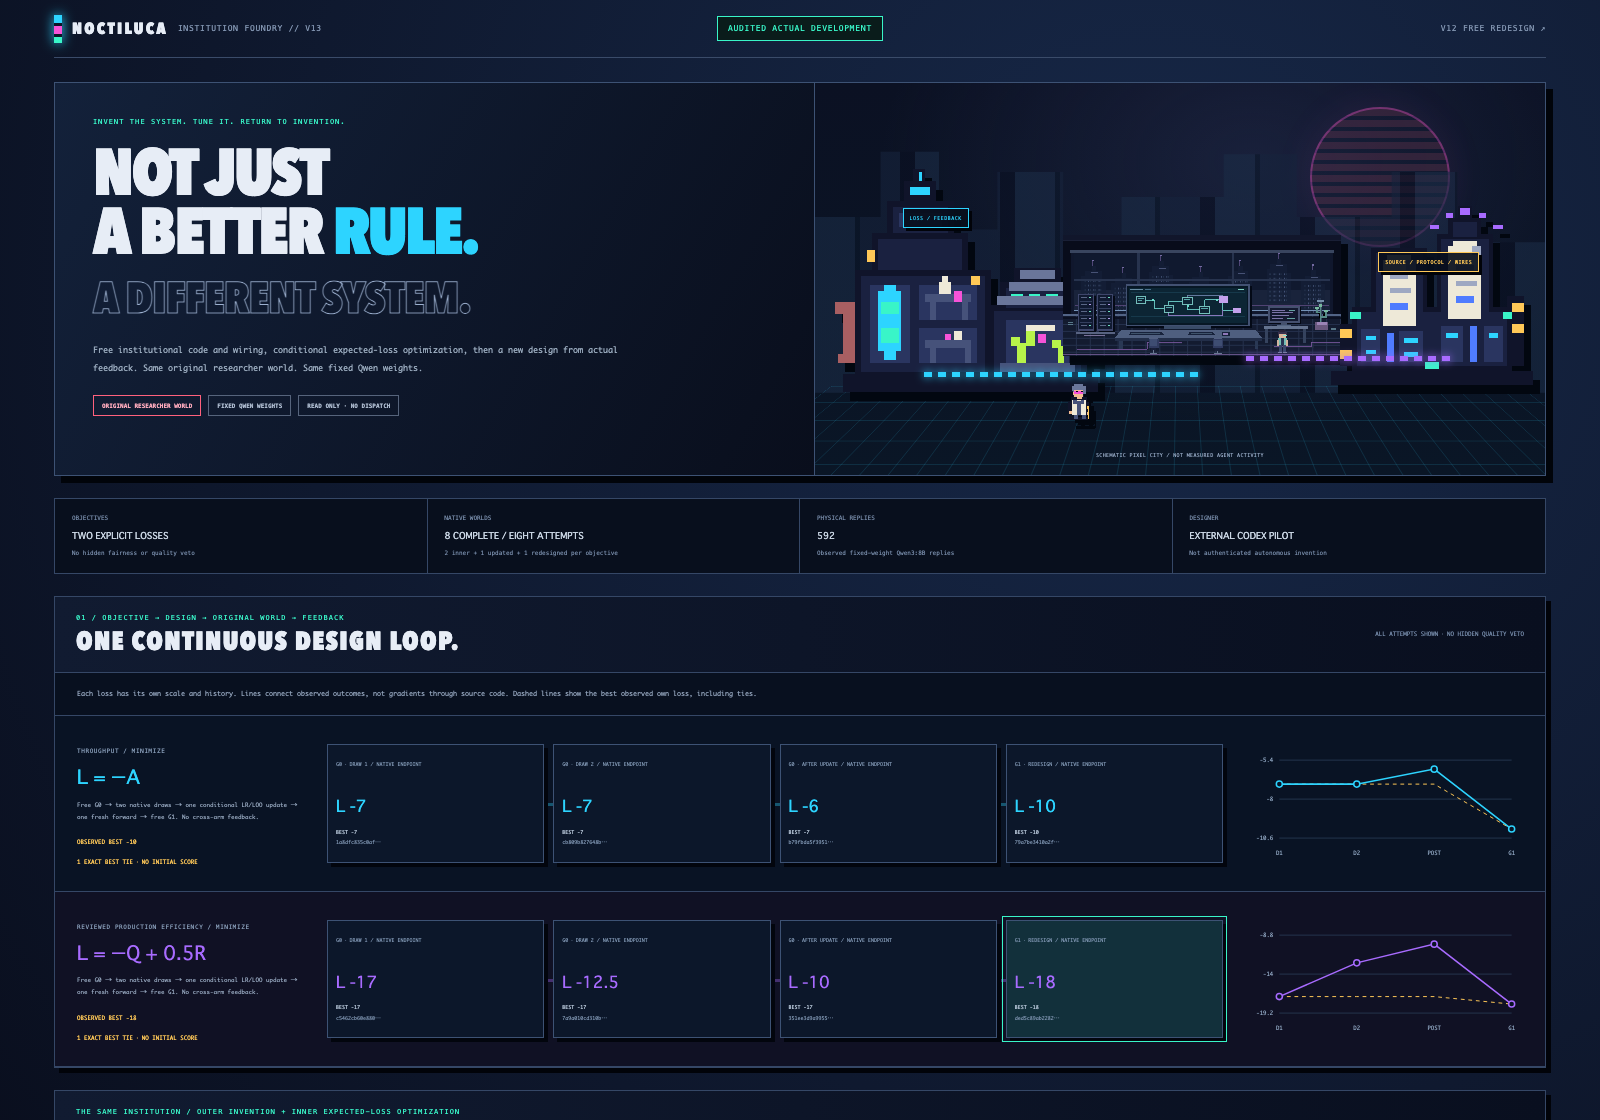
\includegraphics[width=\linewidth]{../game-ui-v2/screenshots/nested-foundry-v13-actual-qa/nested-foundry-v13-actual-overview.png}
\caption{\textbf{Actual English Institution Foundry view of the V13 evidence.}
Cards show the complete eight-world nested case, including worse post-update
draws and external-designer provenance. Pixel city movement is schematic, not
measured researcher motion. This historical capture is bound to V13, not a
claim that the screen displays the later V2 study or that gameplay improves
research understanding. Full-size captures remain in the artifact repository.}
\label{fig:integrated-ui}
\end{figure}

The useful interaction is to move between levels: inspect an objective's
history, select an observation, read the literal institution, follow its graph
and examine which effects reached native scientists. A local editable branch
can start from an observed system; a draft is not executed merely because it
is visible. Runtime validation, an explicit queued job and actual compute
authorization remain separate. Likewise, installing a new institution into
a continuing society is different from evaluating it in a reset world.

This establishes an evidence-reading and design interface, not a completed
management game. No user study, learning benefit, enjoyable gameplay or human
policy-design advantage is demonstrated. Those require separate evaluation.
The longer-term game can make information circulation and institutional
decisions interactive, but it must retain the same identity/state boundary
rather than manufacture a more flattering world for display.
\FloatBarrier

\section{Before scaling: discriminating mechanisms from interface burden}
\label{sec:prescale}
The next stage is not simply more seeds. We first separate three tractable
questions: whether a proposer can submit its intended design, whether an
institution has an actual native consumer, and whether objective-conditioned
revision changes native outcomes. Only the last is new optimization evidence.
The following additions have distinct statuses; they are not folded into the
closed V2 benchmark or its unchanged selection.

\subsection{What the closed record already explains}
A read-only analysis of all 120 V2 statuses retains 64 measured profiles and
nine reference profiles reconstructed from their three affine loss scores.
Those nine reconstructions are not new raw measurements. In the observed
coefficient family $L_{\alpha,\beta}=\alpha A-Q+\beta R$, the original
$C$ coefficients $(4,0.1)$ favor reviewer-free rejection over the observed
high-$Q$ profile. This follows from proxy geometry, not necessarily a weak
optimizer. The map is only over observed profiles; it is not a bound or optimum
for untried dynamic policies (Figure~\ref{fig:observed-objective-map}).

\begin{figure}[t]
\centering
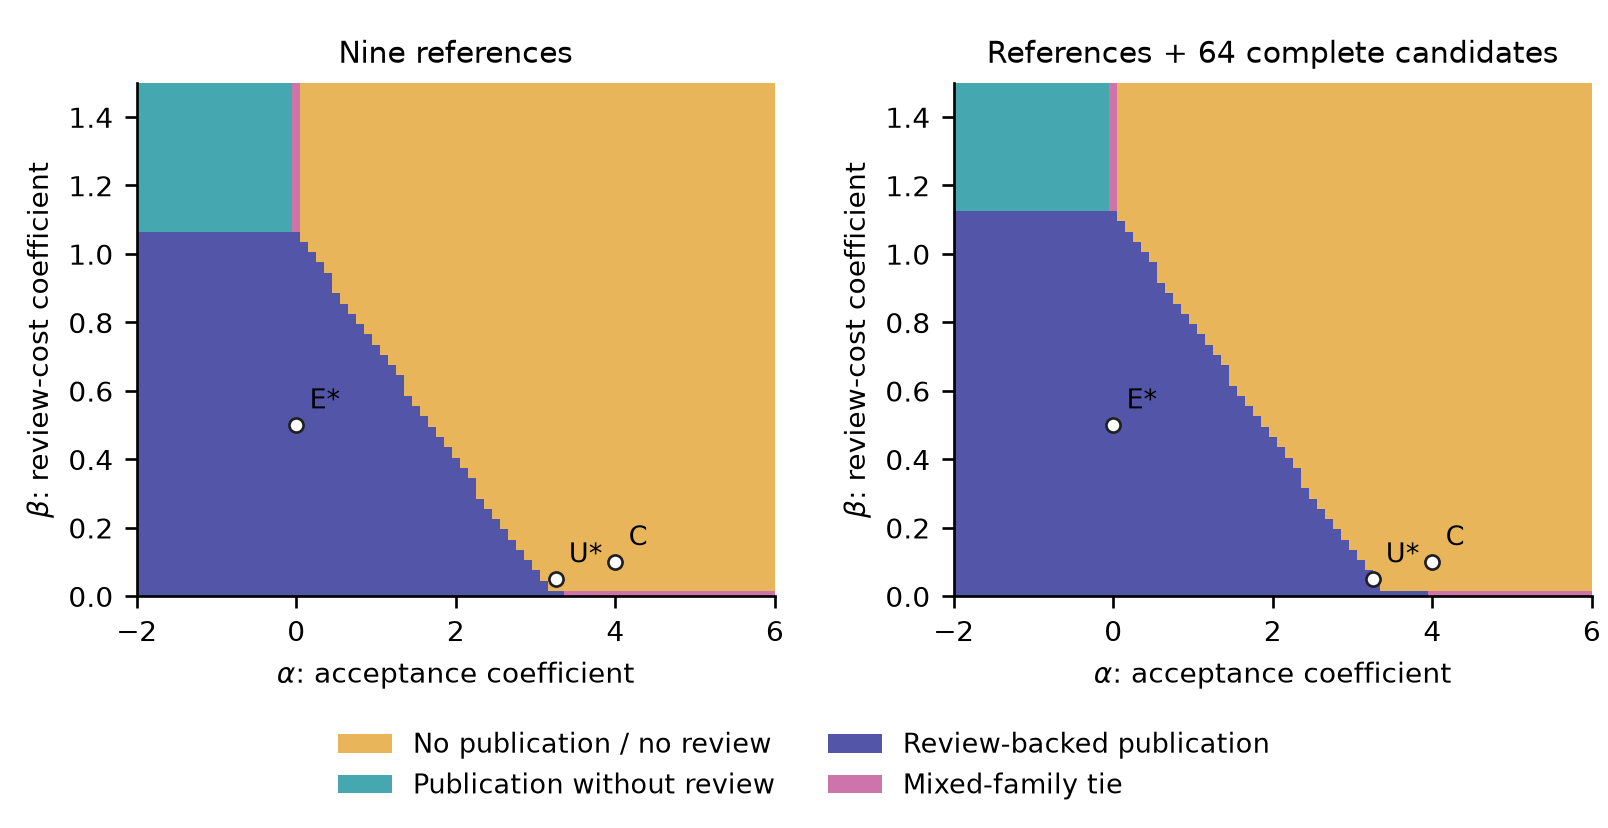
\includegraphics[width=\linewidth]{figures/pre-scale/observed-objective-map-print.png}
\caption{Post-hoc objective geometry over observed development profiles,
not new objective-conditioned search. Left: nine reference-score inversions;
right: those references plus 64 measured completed candidates. Colors identify
observed outcome families, not general policy equivalence. The coefficient
grid is a plotting choice, not additional samples or global optimality.
C is the original V2 loss; E*/U* mark diagnostic formulas, not new searches.}
\label{fig:observed-objective-map}
\end{figure}

Likewise, the numeric failures are not an absence of submission attempts.
Their 384 editor steps contain 47 finish rejections: 43 outside the declared
numeric-only domain and four out-of-range. Of 228 reads, 166 target existing
selection source. This describes a presentation/compliance confound and does
not identify a single proven cognitive or transport cause. A new interface
must be tested prospectively rather than repairing these failed slots.

\subsection{Literal numerical submission: a limited real-backend result}
The new numerical interface asks for exactly six typed coordinate values and
an uninterpreted rationale. Values compile literally to a patch under the same
declared domain; there is no clipping, code repair or implicit baseline. A
complete explicit parent assignment is valid retention. Finite semantic-call
and whole-session wall budgets, durable exact wire bytes, raw responses and
cold replay distinguish known invalid replies from unknown completion.

At pinned source~\code{215311c}, two predeclared local 35B readiness cases both
complete on their first generation call (Table~\ref{tab:numeric-readiness}).
No native world is evaluated. In particular, the E rationale incorrectly
conjectures that limiting delivered history records could directly reduce the
review-count metric; preserving a valid literal submission does not validate
that explanation. The result establishes interface execution for these two
requests, not an optimized loss, general editor readiness or designer competence.
Later runtime changes require a new source-specific certificate.

\begin{table}[t]
\centering\small
\begin{tabular}{@{}lrrll@{}}
\toprule
Case & Prompt tokens & Output tokens & Literal action & Native loss\\
\midrule
T &3196&285&Explicit parent retention&Not observed\\
E &3340&993&Different valid coordinates&Not observed\\
\bottomrule
\end{tabular}
\caption{Actual local 35B numerical readiness, two generation POSTs. Recorded
HTTP call times are 6.972 and 14.056 seconds, excluding separate role loading and
other overhead. Both submissions cold-replay. This is not a search comparison.}
\label{tab:numeric-readiness}
\end{table}

\subsection{A native information-path intervention, not another toy world}
A developer-authored history office now reads actual native papers, statuses
and review summaries, with bounded records per researcher. M0 runs the
producer without delivery; M1 delivers own history; M2 delivers society
history; M3 delays own history an additional year. All retain the original
scientific activities and remove the old example's direct project reassignment.
M2 is not an exactly token-matched inert placebo. Original-world tests with
scripted HTTP/corpus and real isolated code execution verify first direction
input years absent/2/2/3 and full pre-delivery payload equality under different
host clocks. These are software/effect-path tests, not fresh Qwen outcomes.

The finite actual study declares three development seeds and four years,
at most 12 worlds. At the recorded observation on November 9, the first world
has started, initial direction replies exist, and the missing four-year
literature embedding index is being built on CPU. No terminal world
observation is available. This status does not imply completed scientific
results or a continuing live heartbeat in the manuscript.

A separate prospective source implements T/E search over numerical, fixed-graph
code, code/graph and uniform proposals: two generations, at most 16 candidate
worlds plus six fresh references. The selected policies are frozen before at
most 36 four-year unused-seed evaluations. The pilot explicitly fixes original
production/calendar/accounting effects, while permitting institutional
algorithms, entities, memory and routes to change. This is a declared design
domain, not an additional outcome veto or the global expressive ceiling.
Source-specific numerical and staged-editor readiness gates precede dispatch.
At this manuscript revision, this search/evaluation is implemented but not
executed; it supplies no additional optimizer outcome.

\subsection{Verifiable activities and continuity at the same boundary}
An opt-in claim-verification consumer checks an institution's literal assertion
about counts of actual native accept/reject decisions or review records over
a completed interval. It reads the simulator's archive independently of the
candidate's observation or proposed verdict. A correction has a new identity,
retains the false predecessor and binds its verification hash. Retained state
is checked against actual evidence, rather than accepting a designer-seeded
\code{matches=true} flag. Scientific text remains literal; a source-owned
operational review-time field is excluded only from the count-evidence identity.

Original-world/Docker software tests connect authored false assertion,
independent verification, correction and actual next-year researcher input.
This is internally checkable empirical work about the simulated society,
\emph{not} verification of the truth of retrieved scientific papers or a new
scientific-value objective. No default phase or hidden merit gate is added.

Additional scripted native tests place the existing antithetic score estimator
on the current information institution, execute its updated parameter in a
fresh native forward and retain a no-gradient control. A same-society test
changes the history mechanism while preserving researchers, papers, resources,
mechanism memory, RNG state and pending delayed deliveries. These establish
current-boundary connectivity, not new live-model gradients, practical method
advantage, autonomous invention or recursive improvement. The English
pre-scale observatory presents only timestamped journal observations, explicitly
distinguishing a start without a terminal record from a verified completion.

\section{Authority, authoring and measurement diagnostics}
\label{sec:design-diagnostics}
The closed comparisons leave several explanations for limited structural
search: the objective may favor a simple rule, an operation may be unavailable
in the declared domain, the author may misunderstand its execution point,
or the submitted function may fail on native inputs. The following diagnostics
separate these possibilities without adding candidate losses to the earlier
studies or pooling different sources as method replications.

\subsection{Available operations and execution time}
In the information institution, costs execute at phase 80, review at 90,
feature extraction at 100, decision code at 130 and publication at 140.
A late decision function can affect subsequent resubmission and future work,
but cannot remove the current year's completed review operation.

An existing typed review-routing capability binds institution-authored
assignments to the actual submitted papers, eligible reviewers and exact
input-batch hash. However, the earlier fixed-production domain rejects that
implementation as part of its protected production boundary. A prospective
\code{fixed-native-production-review-routing-v2} scope makes this additional
authority explicit while retaining the original planning, production and
accounting semantics. It does not redefine the old domain retrospectively.
Its pre-review snapshot/producer must also precede the actual review stage.

These facts identify what an edit \emph{could} change, not why a previous
designer omitted an unattempted edit. A later source/domain change cannot by
itself establish that earlier non-rewiring was caused by a missing capability.
Nor does extra authority establish that a graph representation is necessary:
an equally authorized policy program with the same callbacks may express the
same computation. Native connection checks use scripted researcher replies
and real isolated execution; they are not autonomous invention results.

\subsection{Eight closed authoring sessions and fixed-input probes}
At source~\code{a2fb13c}, a finite authoring assay crosses T/E, initial versus
one recorded own-history request, and access versus no access to an optional
execution-order reference file. These historical requests are new authoring
inputs, not fresh world observations. Each local 35B session has 16 charged
actions, 8192 output tokens, 40960 context and 1200 seconds. Both condition-specific
readiness sessions pass 29 controls at their own binding.

All eight sessions finish with static-valid explicit submissions, reproduced
by two byte-identical original-source cold audits. Seven change selection
source; one changes four upstream router coordinates. None changes node,
connection or schedule metadata. Five intermediate actions are rejected
within the fixed budget; no slot is refilled and no received code is repaired.

The explanatory file is not read in any of the four access-enabled sessions;
capability-detail files are also unread. Thus this is a comparison of offered
file access, not evidence that understood execution-order information was
ineffective. Its request-bound decode seeds also differ between conditions,
so it is not a common-random-number treatment estimate.

Separate network-disabled, read-only Docker probes use four saved native
selection inputs containing 2, 7, 9 and 11 papers. The original selector first
replays exactly on all four. Each candidate selector is then tested on those
same frames, resetting to the recorded input/state rather than carrying the
candidate's state through years. Table~\ref{tab:authoring-fixed-probes} retains
all eight candidates. No probe commits a native decision, runs an upstream
mechanism or evaluates a new scientific world.

\begin{table}[htbp]\centering\small
\caption{All authoring submissions and partial selector probes. H0 is the
initial request; H1 contains a recorded history. File means optional access,
not actual reading. Rows are not native-world validity or loss results.}
\label{tab:authoring-fixed-probes}
\begin{tabular}{@{}llll>{\raggedright\arraybackslash}p{.49\linewidth}@{}}
\toprule Loss & History & File & Edit & Fixed-input result\\\midrule
T & H0 & No & Source & Accepts all 29 addressed papers\\
T & H0 & Yes & Source & Accepts all 29 addressed papers\\
E & H0 & Yes & Source & \code{KeyError: world} on all 4 inputs\\
E & H0 & No & Numeric & Unchanged selector rejects 29; edited upstream is not executed\\
T & H1 & Yes & Source & Empty-cycle output on all 4 nonempty inputs; identity coverage fails\\
T & H1 & No & Source & Accepts all 29 addressed papers\\
E & H1 & No & Source & Accepts one per input, rejects the remaining 25\\
E & H1 & Yes & Source & Accepts all 29 addressed papers\\\bottomrule
\end{tabular}\end{table}

Of 32 candidate function calls, 28 return and 24 cover every addressed paper.
These are component checks, not six valid whole institutions. In particular,
the numerical candidate's modified upstream is not exercised by a selector-only
probe. Runtime exceptions and empty outputs show why successful static
submission cannot certify arbitrary code's behavior on actual inputs.

Generated explanations also differ from operative effects. One plan proposes
stricter late selection to avoid earlier review work. Another source raises
\code{final\_score} to at least 10, but the E loss reads original reviewer scores,
not that authored field. A later source comment correctly acknowledges the
late selector's lack of direct review-count control. These are literal
observations about particular programs, not a universal diagnosis of the
model's reasoning or evidence of measured loss improvement.

Authoring uses 110 chat POSTs with 2,225,666 reported input and 23,017 output
tokens; readiness uses 58 POSTs with 618,249 input and 3,574 output tokens.
The interval from first start to last chat response is 1861.22 seconds.
Ten separate empty-prompt loads complete with unreported token counts, not
observed zero usage. The assay and probes make no researcher-model calls and
produce no new candidate losses. Inline order context and more detailed ABI
cards are later prospective interfaces, not retroactive changes to this assay.

\subsection{A fixed measurement function can have endogenous observations}
The measurement code is immutable within a study, but the observations it
receives need not be institution-independent. For the original-review proxy,
\begin{equation}
 Q(\tau)=\sum_{\substack{p\in\mathcal A(\tau)\\|\mathcal R_p(\tau)|>0}}
  \frac{1}{|\mathcal R_p(\tau)|}\sum_{j\in\mathcal R_p(\tau)}y_{pj},
 \label{eq:endogenous-panel}
\end{equation}
with zero contribution for an accepted decision without reviews, as defined
by the adapter. Both the accepted set $\mathcal A$ and reviewer set
$\mathcal R_p$ can depend on the institution. Excluding an authored final
score from Q therefore does not turn Q into independent scientific quality.

A read-only analysis revisits the 49 physical worlds of the closed \code{62388a7}
T/E pilot. It reconstructs A/Q/R from the 44 completed four-year checkpoints,
retains five partial failures without imputing complete outcomes, and checks
the full 1859-file inventory against the original-source full audit. These
records contain 217 reviewed and 46 unreviewed accepted decisions, not 263
independent papers or new world replications.

For each already observed review panel, we enumerate mean-score readouts of
all subsets of size $k$. Accepted papers and actual review work stay fixed.
A uniformly selected subset has the same expected mean as the original panel;
the minimum and maximum are sensitivity endpoints and can require hindsight.
The analysis neither simulates choosing those reviewers in advance nor
subtracts the cost of reviews that were actually performed.

Twenty-four completed worlds have a nonzero one-score Q-readout envelope.
Figure~\ref{fig:fixed-panel-readout} shows all three old evaluation seeds for
the E/numerical selection and reviewed accept-all. Within each row, the
recorded accepted set is fixed; artifacts and responses need not match between
rows. At seed 51001, for example, original Q values are 39.667 versus 40.667,
with one-score readout ranges 39--41 versus 39--43. These are not confidence
intervals, independent quality estimates or an explanation of the observed
between-policy difference. They do not invalidate that measured difference.

\begin{figure}[htbp]\centering
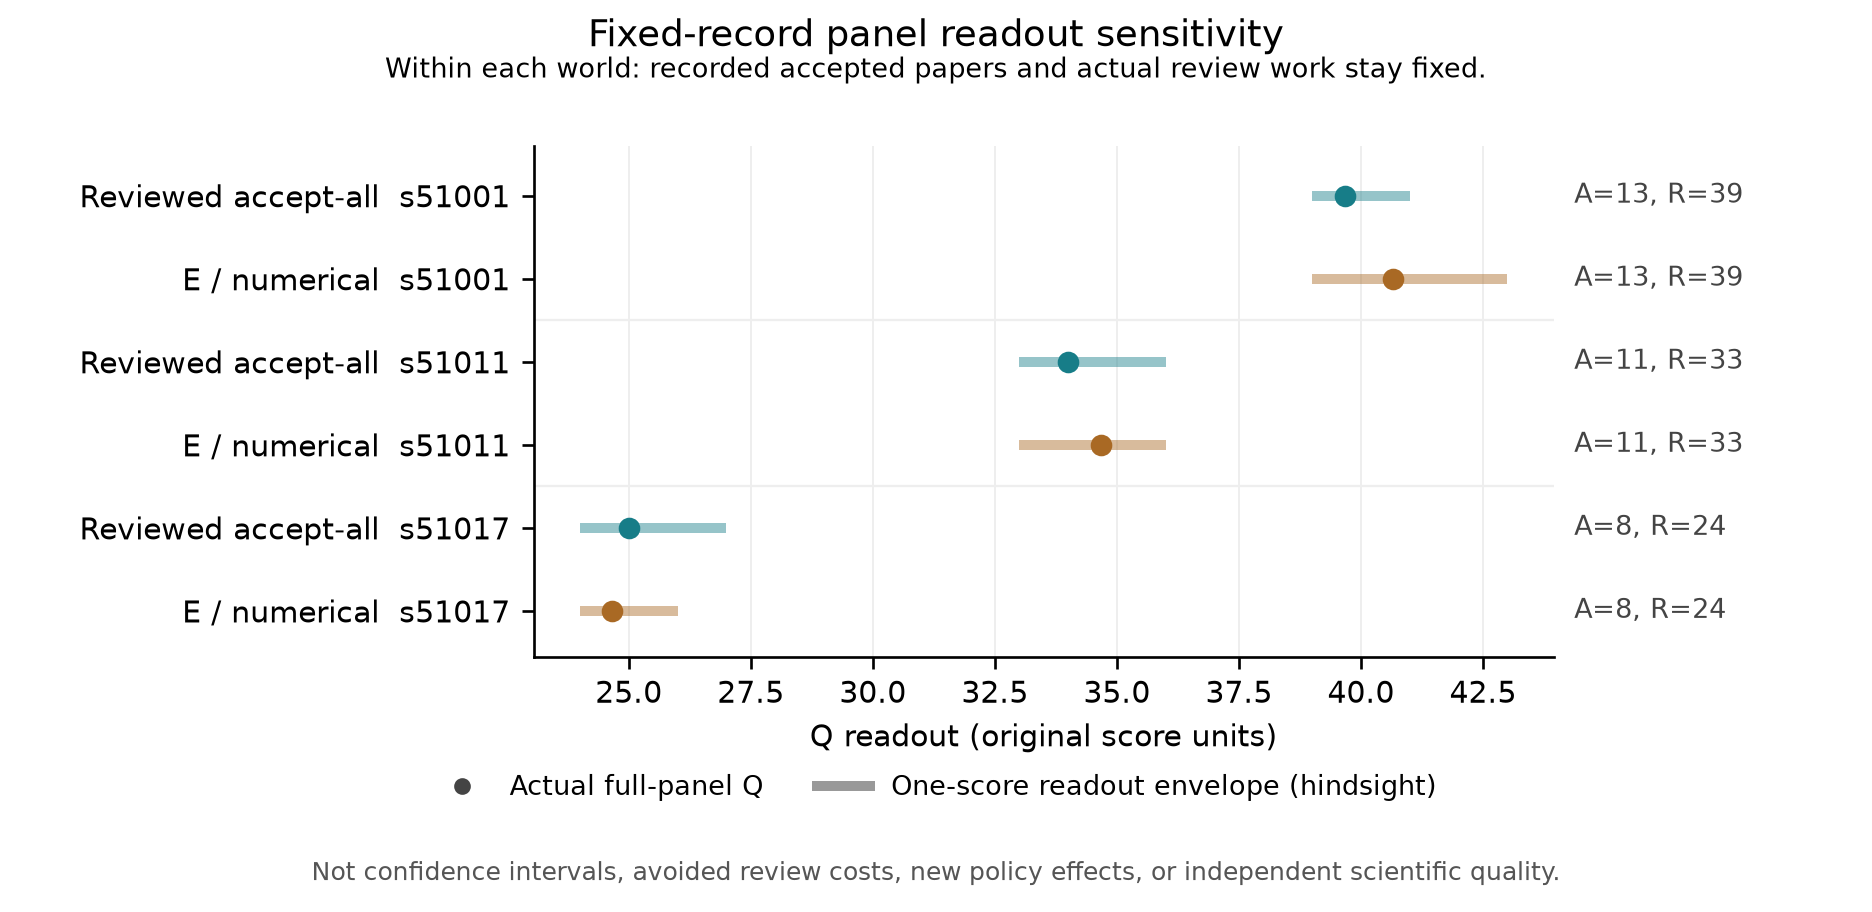
\includegraphics[width=\linewidth]{figures/native-panel-sensitivity-v1/fixed-panel-readout.png}
\caption{\textbf{Recorded panel readout sensitivity.} Dots are actual full-panel
Q; bars reuse one score per already reviewed accepted decision, with hindsight
endpoints. Actual A and R remain unchanged. This is not a reviewer-routing
intervention, reduced review cost, new optimization or scientific quality.
Both original-source analyses and both PNG/SVG builds reproduce identically.}
\label{fig:fixed-panel-readout}
\end{figure}

The practical implication is to name the optimization target precisely.
T/E remain legitimate declared proxies; this diagnostic adds no new loss,
fairness condition or adoption veto. A separate blind evaluator could measure
another fixed-panel opinion, but would not itself verify scientific truth.
Claims about knowledge gain would require an independently justified
measurement or actual verification activity within an extension of the native
researcher world. The prospective routing-authority closed-loop study has its
own finite protocol; its in-progress observations are not counted here as a
completed comparison.
\FloatBarrier

\section{Native code execution and the support of the objectives}
\label{sec:native-loop}
Permitting arbitrary code is not the same as obtaining a working institution,
and obtaining a working institution is not the same as answering an important
optimization question. This section separates these issues in a later native
campaign and a read-only analysis of the earlier completed T/E cohort.
The loss definitions remain unchanged; no participation, novelty or fairness
condition is added to the optimizer's acceptance criteria.

\subsection{A stopped routing-authority campaign}
The new campaign retains the original five fixed Qwen3-8B researchers, the
SciEvo literature and four-year Simulation. It crosses T/E with numerical,
fixed-graph source and code-and-graph design. Two proposals per arm and eight
references are declared in advance. The references include original reviewed
accept-all and typed one- and two-reviewer accept-all institutions, giving
simple controls access to the same new review-routing authority as generated
institutions. These controls change actual review work, not a retrospective
subsampling of already paid reviews.

All eight reference worlds complete. Of twelve declared proposal slots,
eleven are submitted: five complete native execution and six fail technically.
The final numerical T proposal is never submitted because its required fresh
interface calibration fails on the E control. That response is a final HTTP 200
envelope with \code{done=true}, a length termination and 8192 reported output
tokens, but no complete literal submission. The campaign stops at that point;
its unsubmitted slot is neither refilled nor assigned a loss.
Table~\ref{tab:native-stopped-slots} retains all twelve slots. Two cold
stopped-prefix audits agree on the nineteen physical worlds and their original
responses, checkpoints and measurements. This audit scope verifies a stopped
experiment, not normal completion of its planned search and evaluation.

\begin{table}[htbp]\centering\small
\caption{All declared slots in the stopped native campaign. Numbers are
development losses, not unused-seed results. Technical nulls have no imputed
loss; generation labels index each arm, not the global dispatch sequence.}
\label{tab:native-stopped-slots}
\begin{tabular}{@{}llll@{}}
\toprule Objective & Allowed design & Generation 0 & Generation 1\\\midrule
T & Numerical & $-7$ & Not submitted\\
E & Numerical & $-11.167$ & $-11.167$\\
T & Fixed-graph code & $-2$ & Float used as index\\
E & Fixed-graph code & Missing world envelope & $-11.167$\\
T & Code and graph & Missing feature key & Missing world envelope\\
E & Code and graph & Float used as index & Float used as index\\\bottomrule
\end{tabular}\end{table}

Seven of the eight code-permitted submissions change source, and the remaining
one changes numerical router coordinates. None changes connections, node
membership or scheduling. The completed fixed-graph T submission is the
numerical-only edit; the completed fixed-graph E submission changes source.
Therefore neither the method label nor static acceptance establishes that
structural freedom was exercised successfully. The six execution failures
are three float-index errors, two missing output envelopes and one missing
feature-key error. Their literal programs remain unmodified.

The nineteen worlds produce 1796 completed scientist responses, with
1,615,207 reported input and 181,308 output tokens. Separate auxiliary records
contain 256 editor-readiness, 112 staged-proposal, 13 numerical-readiness and
three numerical-proposal intents, plus 25 designer and nineteen scientist
loads. Unreported usage on load calls is unknown, not zero. Readiness and
proposal costs are not silently excluded because the campaign stopped.

\subsection{Separate evaluation of the available submissions}
The stopped campaign has four arms with at least one completed submission;
the two code-and-graph arms have none. A separately frozen study selects the
minimum assigned development loss within each available arm, preserves all
ties, and uses the earliest tied submission. It then evaluates those fixed
policies and six references at seeds 62001, 62011 and 62017, whose prior use is
checked before dispatch. No new designer proposal is generated. Thirty
physical jobs are declared without semantic deduplication. An unavailable arm
has no policy and no score; it does not inherit the seed or a hand reference.

This study evaluates policies available after a stopped prefix. It cannot
complete the missing proposal, establish an equal-budget method comparison or
turn three evaluation seeds into independent design histories. Its results
are integrated only after its own scientific terminal and independent cold
audits close. The new development loop described below does not receive these
unused-seed losses.

\subsection{Execution feedback without host repair}
The execution failures motivate an optional component-testing interface, not
an automatic repair of received programs. A developer bank binds 24 literal
native inputs to three earlier development references, two components and
four saved years. A proposed code artifact can be tested in the existing
network-disabled container; the input, received code, returned value or exact
exception, timeout and charged attempt are retained. Component tests do not
replace native evaluation or define another loss.

Three real-container diagnostics illustrate both utility and limited support.
On the same saved year-one input, the baseline reproduces its recorded output
and a retained missing-envelope program fails. A retained float-index program
returns because that input's paper batch is empty: a passing component test
does not show that the program handles a later nonempty batch. Multi-year
coverage is therefore useful, but still cannot certify a whole trajectory
whose inputs change under a new institution.

A prospective post-edit mode connects literal edits to a fixed suite of four
saved yearly inputs, with at most eight component attempts per proposal.
Errors and compact results enter the next designer prompt; the complete
records remain archived. A failed component test neither vetoes submission
nor causes the host to wrap, revert or replace the generated source. Edits
after the component allowance remain permitted and explicitly untested.
Scripted full-path tests connect calibration, the public certificate API,
the production role factory, the next feedback-bearing request and cold
replay. They show software connectivity, not that the actual designer can
repair its code or improve a native objective.

A new finite development campaign declares four own-history proposals,
three fresh strong references and a seven-world ceiling. Its calibration
declares this optional mode without executing component code. It waits for
the preceding evaluation's independent closure before any model inference.
The reused development seed is not held out. Successful closure, self-repair
and objective improvement remain separate empirical questions.

\subsection{Why different proxies can select the same rule}
Fix the submitted records, their observed review scores and actual review
work $R$. Write $z_i\in\{0,1\}$ for accepting record $i$ and $q_i\geq0$ for
its original mean review score, with $q_i=0$ for an unreviewed record. Then
\begin{equation}
 L_T(z)=-\sum_i z_i,\qquad
 L_E(z)=-\sum_i z_i q_i+\tfrac12 R.
 \label{eq:conditional-accept-all}
\end{equation}
Both conditional losses are minimized by accepting every record; an acceptance
with $q_i=0$ ties under E. Different coefficients therefore need not imply
different acceptance rules. An improvement over the initial threshold rule
alone is weak evidence for a need to invent a complex institution, making
accept-all with the same actual authority an essential control.

This is not a global optimum of the persistent world. An institution can
change reviewer assignments, actual work, future submissions, information and
resource trajectories, which are fixed in the conditional statement.
Moreover, changing the reviewer panel changes the observed $q_i$ itself.
Neither the algebra nor a reduction in E establishes improved scientific
truth. Adding an acceptance penalty, a blind observer or a participation term
would define a new prospective objective, not correct this experiment's loss.

\subsection{Observed annual resource and activity support}
An original-source readout of the earlier closed T/E cohort checks all 176
saved annual checkpoints from its 44 complete physical worlds against the
existing full audit. Five partial failures are retained without complete
outcomes. All 880 observed actor--year boundaries are active; all 44 final
activity stocks are five. Table~\ref{tab:native-resource-support} shows the
individual year-end resource range, not only pooled final totals.

\begin{table}[htbp]\centering\small
\caption{Saved annual support in the earlier 44 complete worlds. Each year
contains 220 actor observations. Extrema can come from different actors and
worlds; rows are not a single actor's trajectory.}
\label{tab:native-resource-support}
\begin{tabular}{@{}lrrr@{}}
\toprule Year & Active / observed & Minimum resources & Maximum resources\\\midrule
1 & 220 / 220 & 90 & 150\\
2 & 220 / 220 & 75 & 200\\
3 & 220 / 220 & 55 & 250\\
4 & 220 / 220 & 30 & 300\\\bottomrule
\end{tabular}\end{table}

Two source-bound readouts and two portable numeric exports agree exactly.
All recorded initial-funding fields are 100; repeated stock fields are not
new funding allocations. The historical within-year resource ledger was
disabled, so saved boundaries cannot exclude temporary inactivity or identify
within-year minima. Nor do 44 completed worlds constitute 44 independent
optimizer histories or show that other institutions could not reduce activity.
The final-activity component alone cannot distinguish these observed completed
worlds. Increasing their seed count is not by itself a remedy for an
unobserved or structurally flat target. A more informative main comparison
must first identify a consequential information, action or timing opportunity
in an extension that retains the persistent researcher world.
\FloatBarrier

\section{A delivered information intervention is not necessarily an effective one}
\label{sec:native-advice}

The count/content study changes some inputs without exceeding strong rules.
Before attributing this to absent information or launching a larger search,
we test whether a particular institutional message reaches the relevant native
decision at the intended time. This is a developer intervention, not a newly
invented institution or an independent optimization history.

\paragraph{Fixed contrast and native world.}
At source\code{5925d5b}, three original four-year worlds use the same five
Qwen3-8B researchers, explicitly reused development seed61001, base30 resource
profile, M1 history, conserving equalization and unchanged T/U measurement.
The literal message recommends choosing a permitted short-duration topic; it
does not change the displayed catalog, choose a topic for a researcher or
overwrite project dates. The three conditions cut delivery, deliver at phase2
before the first direction choices, or deliver at phase235 after those choices.
The message and all three conditions are fixed before dispatch, not chosen
from favorable responses. A permission-only preparation stop precedes the
separately recorded successful launch; no scientific slot was consumed there
or replaced. All three worlds subsequently close normally.

\begin{table}[t]
\centering\small
\begin{tabular}{lrrrrr}
\toprule
Condition & Advice in inputs & Shortest choice & Mean duration & T & U\\
\midrule
Cut &0/10 &4/10 &2.6 & $-7$ & $-4$\\
Early &10/10 &4/10 &2.6 & $-7$ & $-4$\\
Late &5/10 &4/10 &2.6 & $-7$ & $-4$\\
\bottomrule
\end{tabular}
\caption{All three literal advice-timing controls. Advice presence is checked
in actual direction-request inputs, not inferred from node execution.
Duration is the selected topic's displayed catalog duration in years, averaged
over ten requests per world. Shortest is relative to that request's permitted
catalog; following the advice is not a validity requirement. The late message
is absent from first-year direction inputs, as declared. These are one-seed
developer contrasts, not independent search replications.}
\label{tab:native-advice}
\end{table}

\paragraph{Delivery established; the proposed choice effect absent here.}
All30 direction requests are uniquely joined to their original stored memories
and displayed catalog. Early and late delivery each store five addressed
instruction records; cut stores none. The exact literal text occurs in0/10,
10/10 and5/10 direction inputs, respectively. Nevertheless, every corresponding
actor/year chooses the same topic and catalog duration across all three worlds
(Table~\ref{tab:native-advice}). Each chooses a shortest displayed option on
four of ten requests, with mean selected duration2.6 years, and all yield
T=$-7$/U=$-4$. Non-shortest choices are not schema violations: the message is
advice, not a mandatory native law. We retain those choices and their losses
rather than rewriting them to satisfy the instruction.

\begin{figure}[t]
\centering
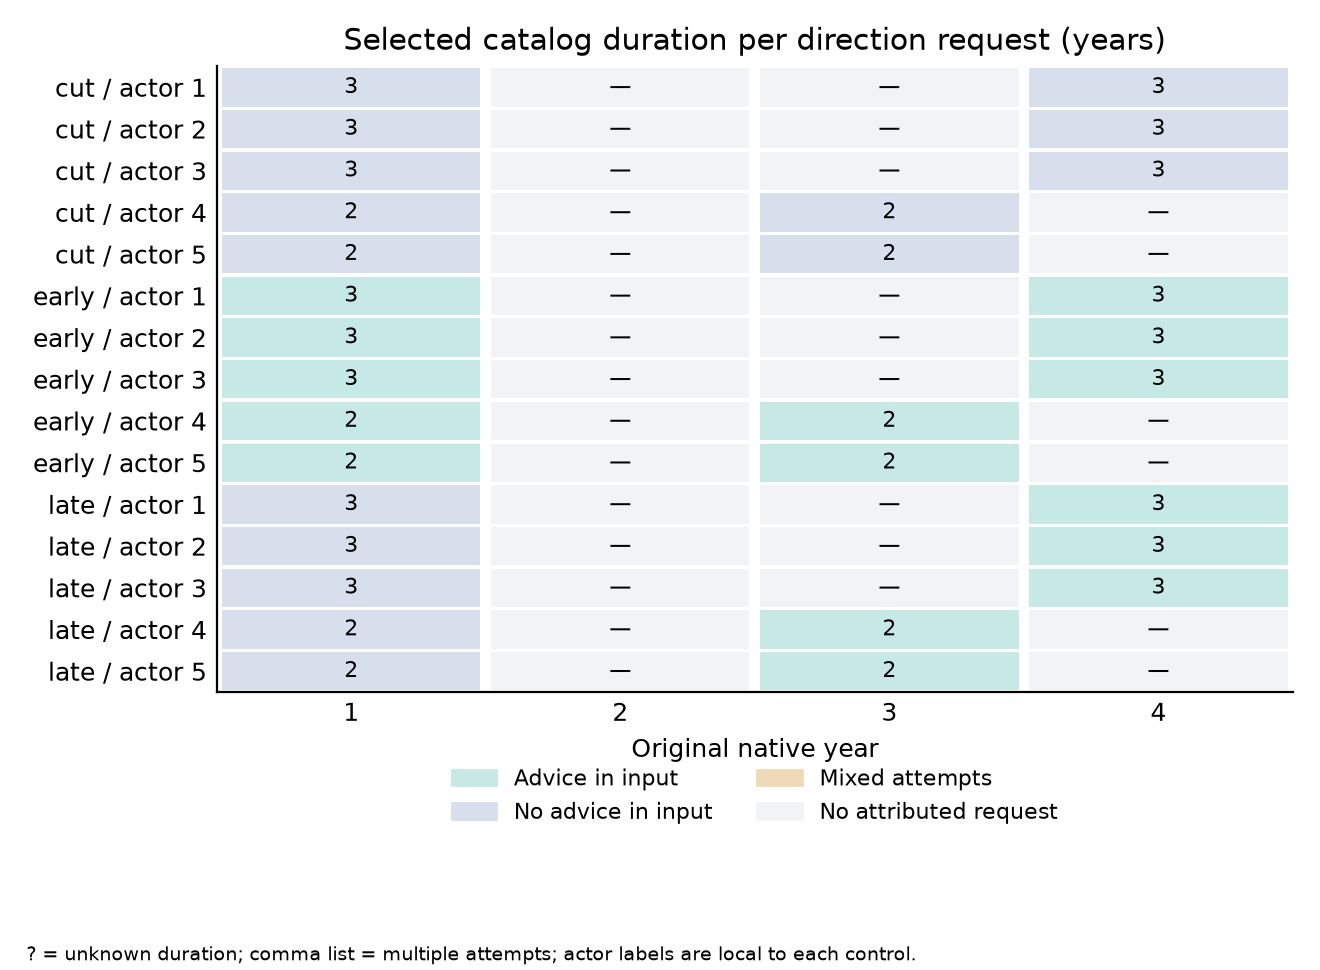
\includegraphics[width=\linewidth]{figures/native-instruction-timing-v1/choice-years.png}
\caption{Actual annual direction-input delivery and catalog-duration choices
in the three closed native worlds. The original displayed catalog and literal
received action determine each point. Delivery varies at the declared times;
the observed selected durations coincide. This supports a scoped delivery/choice
distinction, not a general inability of information institutions to affect
researchers or a causal account of why this message did not change topics.}
\label{fig:native-advice}
\end{figure}

\paragraph{Equal selected choices do not imply equivalent worlds.}
The complete ordered model-input and literal-response sequences differ among
all three worlds. Cut has129 completed scientist replies, early and late130
each. Total author resources at year4 are350,310 and350, respectively. Thus
unchanged topics, durations and T/U are weaker than behavioral equivalence or
identical resource trajectories. Resource diagnostics do not add an adoption
veto or another term to either optimization loss.

\paragraph{Audit, costs and inference boundary.}
Two original-source cold audits and two cost projections agree; the choice,
effect and complete-input exports and repeated summary/figures also agree.
Actual native execution takes about24min, followed by about1m15s of cold/report
closure. There are389 scientist replies with360734 input and38542 output
tokens;63873 cached input tokens are a subset. The unchanged content observer
uses39 separate requests. Tokenless model-load costs remain unknown; there
are no designer proposals. The result establishes that this literal message
was delivered and did not improve these particular choices or T/U at this
seed. It does not establish general instruction ineffectiveness, equal full
behavior, scientific quality, a policy ranking or a benefit of graph search.
All exact data, message identity, source and closure receipts are retained in
\path{research/data/native-instruction-timing-v1/}.
\FloatBarrier

\section{Capacity-limited native search preserves a strong allocation rule}
\label{sec:native-capacity}
\subsection{A separate activity objective under original production laws}
The preceding count/content search does not identify a useful objective-to-system
distinction. We therefore conduct a separately declared native pilot with
existing capacity limits, not a retrospective change of its losses. Five
original Qwen3-8B university researchers operate for four years over the same
103,107-record corpus, with base30 balanced resources. The original
\code{papers\_per\_project}=2 cap permits partial submissions. Fixed funding
at fraction0.2 supplies one total annual award slot across programs. Native
research cost remains10 when an active researcher has a working project;
the original per-paper flow has no direct submission debit. Neither a paper
fee nor a new resource law is activated to force a trade-off.

Alongside $T=-A$, let $I_{iy}$ be one exactly when founder$i$ is author-capable
and has\code{is\_active}=true at the end of year$y$, and zero otherwise.
Define the separate loss
\[
 P=-\sum_{y=1}^{4}\sum_{i\in F} I_{iy},
\]
where $F$ is the initial five-researcher cohort. New actors do not enlarge
the cohort. The formal minimum is$-20$; the indicator does not certify
resource sufficiency, useful work or continuous survival. In particular,
native zero-resource activity semantics are preserved. P is an objective
in its own search, not an additional constraint on T or an adoption veto.
Every complete world receives both scores from its original checkpoints.

Five common developer rules precede two own slots per objective at explicitly
reused development seed61001. All rules use their declared native authority:
reviewed accept-all with equalization; its transfer cut; no-review accept-all
with equalization; and reviewed accept-all with reserve-proximity or
completion-priority allocation. The latter rules conserve resources and seek
a pre-cost reserve of21. They are strong hand controls, not generated inventions.
Each actual editing parent minimizes the assigned loss over common references
and its own history; all four slots start from reserve-proximity. Final selection
is instead restricted to complete own literal submissions, including retention,
with the earliest tie and no reference fallback. The local35B designer has
16 proposal steps per slot and64 optional historical component probes.
Initial and four history-bearing technical calibrations precede dispatch.

\subsection{All submissions, strong ties and a real execution failure}
All four slots submit literal programs. Three complete native execution;
P/g1 fails and receives neither a numerical loss nor a replacement. Both
original cold audits and cost projections agree, as do two exports of each
score, effect, input and preference analysis.
Table~\ref{tab:capacity-all} retains the full comparison.

\begin{table}[t]
\centering\small
\begin{tabular}{lrrl}
\toprule
System or own slot & T & P & Annual active founders\\
\midrule
Reviewed all / equalization & $-10$ & $-12$ & 5,5,1,1\\
Reviewed all / transfer cut & $-10$ & $-12$ & 4,4,2,2\\
No-review all / equalization & $-10$ & $-12$ & 5,5,1,1\\
Reviewed all / reserve-proximity & $-12$ & $-15$ & 5,5,3,2\\
Reviewed all / completion-priority & $-12$ & $-15$ & 5,5,3,2\\
T/g0; selected T & $-12$ & $-15$ & 5,5,3,2\\
P/g0; selected P & $-12$ & $-15$ & 5,5,3,2\\
P/g1 & --- & --- & Technical null after year2\\
T/g1; ties T/g0 & $-12$ & $-15$ & 5,5,3,2\\
\bottomrule
\end{tabular}
\caption{All nine physical attempts in the capacity pilot. Lower losses are
better. The failed world has two saved annual boundaries and recorded work
in year3, not a completed four-year outcome. Equal sums for the first three
rules conceal different activity paths. All complete own submissions tie
both strong allocation rules; there is no generated-policy advantage.}
\label{tab:capacity-all}
\end{table}

No own submission changes nodes, connections or schedules. T/g0 replaces
the already all-accept selection source with unconditional acceptance and
constant final score1. T/g1 retains the mean native review score while
rewriting unconditional acceptance. P/g0 likewise retains that mean and
replaces direct field access in the allocation code with existing-value
defaults. These literal edits do not establish a new allocation algorithm.
The full scientist input sequences of P/g0, T/g1 and both strong allocation
references are identical at this observed history, with identical literal
response choices; full provider envelopes are not identical. T/g0 has a
different full input sequence despite the same T/P and activity path.
Observed input equality is not program equivalence on all possible states.

P/g1 attempts a different operation. Its final allocation code includes
initial-founder support and a virtual-source fallback. In year3 it emits
two transfers of10 from the nonexistent actor\code{system}. The native
conserving-transfer receiver rejects the batch because endpoints must be
existing author-capable actors. The original code result and two committed
annual boundaries are retained; partial work is not promoted to a complete
loss. This is an authored invalid command, not evidence that the framework
silently repaired the institution or that the policy performed poorly on P.
Four component probes of that final artifact had returned on historical
fixtures. Their success did not certify the later native consumer or its
trajectory: local code return and valid downstream scientific execution
are distinct tests.

\begin{figure}[t]
\centering
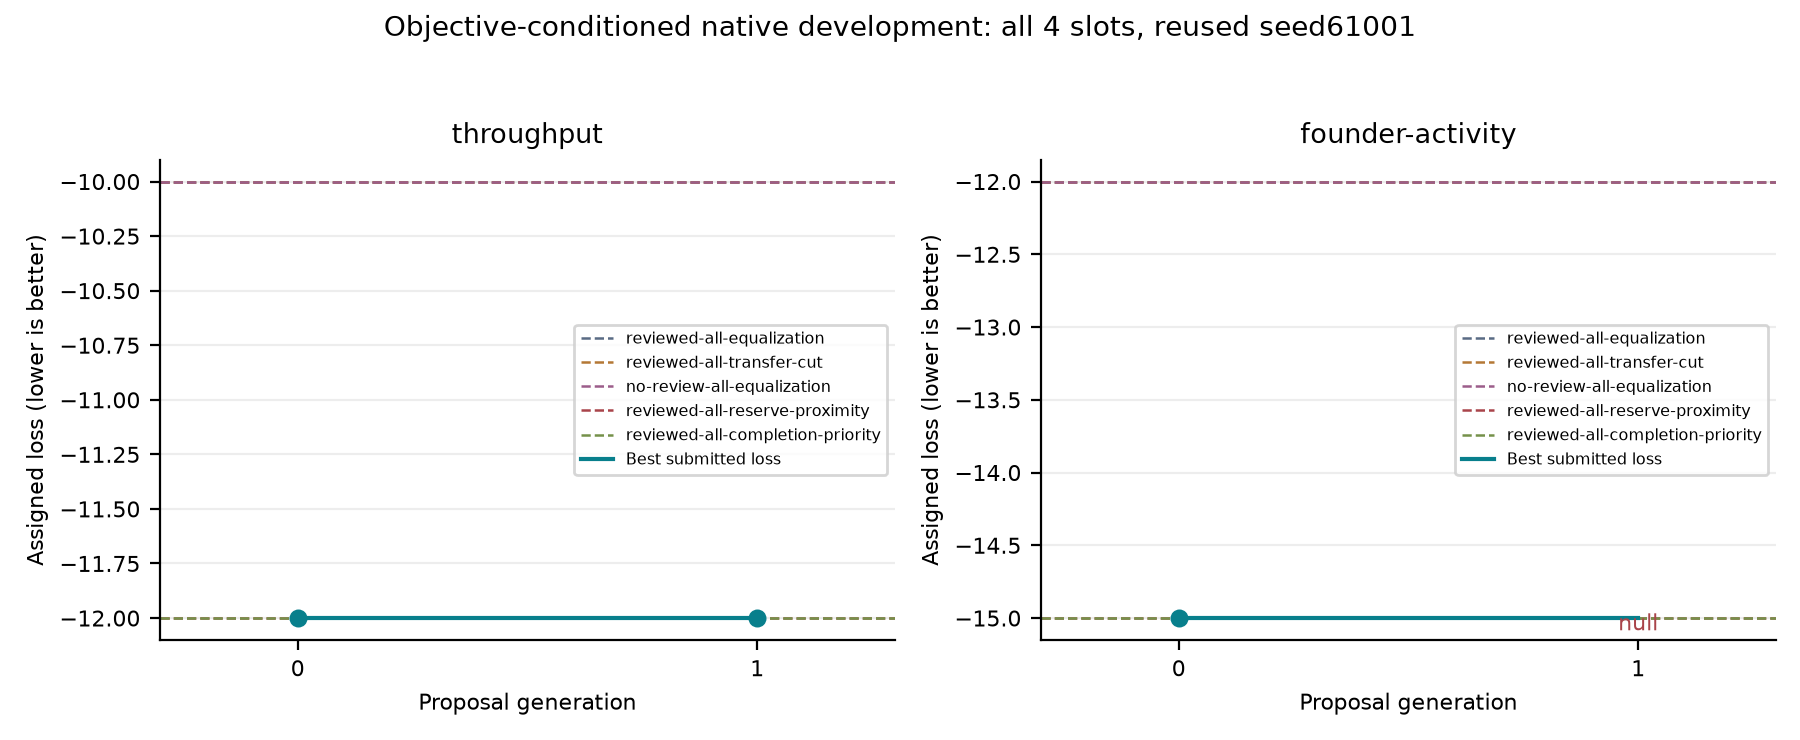
\includegraphics[width=\linewidth]{figures/native-capacity-objective-loop-v1/objective-loss-paths.png}
\caption{Both actual objective-conditioned search paths, all five coincident
reference labels and the P/g1 null. The first own proposal already ties the
strong editing parent; the flat path is not an improvement from that parent.
There is one design history per objective, not independent optimizer replication.}
\label{fig:capacity-paths}
\end{figure}

\subsection{What the common score point does and does not explain}
The eight complete worlds have only two observed score pairs:
$(-12,-15)$ for the two strong controls and three own submissions, and
$(-10,-12)$ for the other three controls. The first strictly dominates the
second in both recorded coordinates. Consequently, every hypothetical
raw-unit linear mixture $wT+(1-w)P$, $0\leq w\leq1$, has the same minimizing
score group in this archive (Figure~\ref{fig:capacity-geometry}). This is an
exact finite-record calculation, not optimization at an interior weight,
a global Pareto frontier or evidence that T and P are intrinsically aligned.
The search did not explore materially different complete organizing systems.

\begin{figure}[t]
\centering
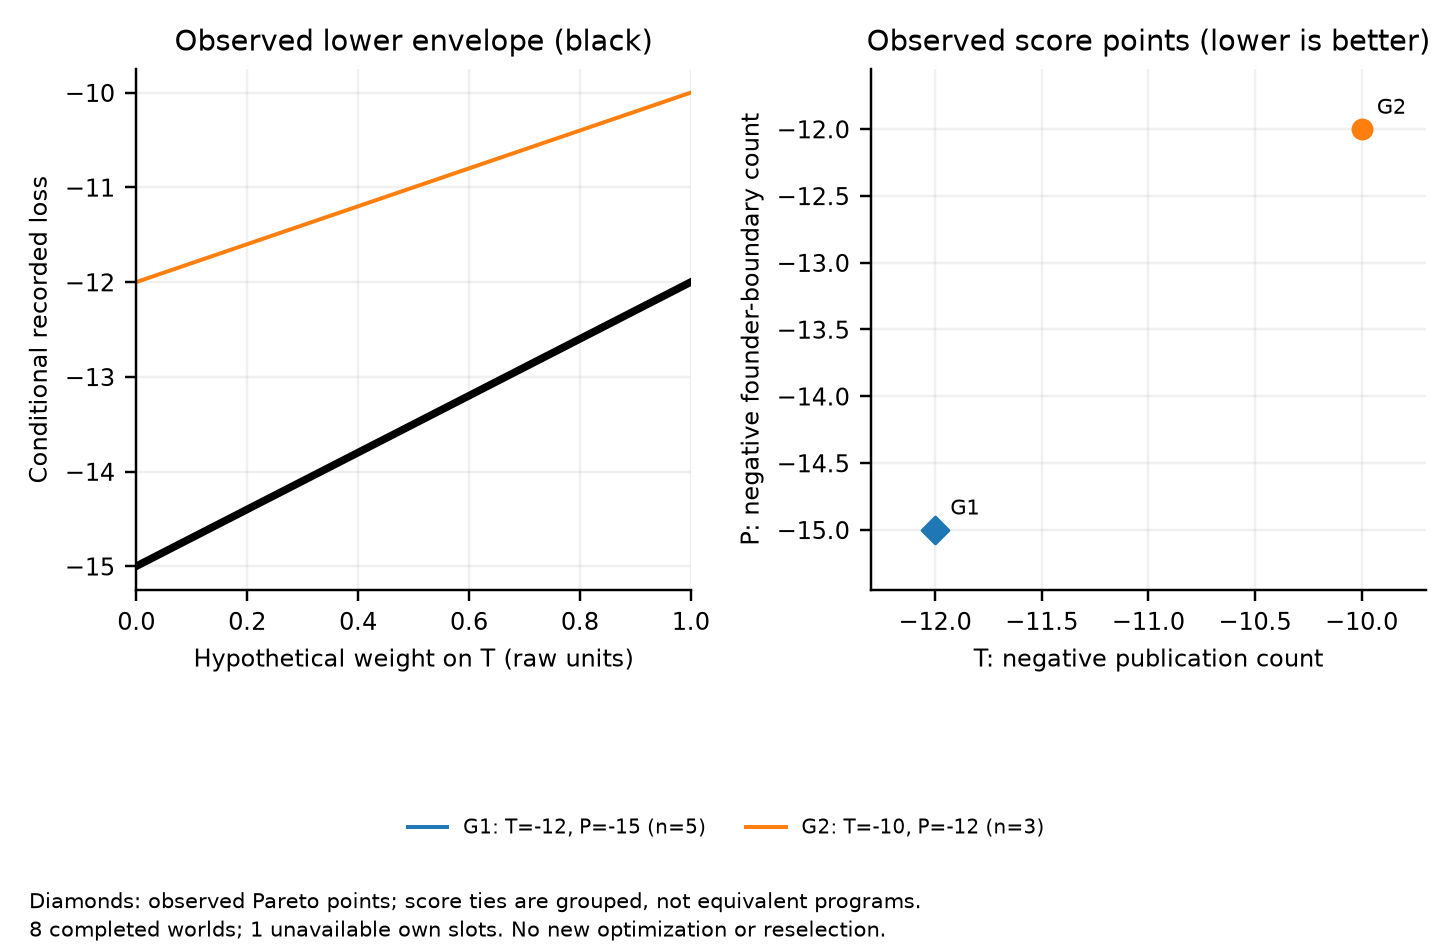
\includegraphics[width=.94\linewidth]{figures/native-capacity-objective-loop-v1/observed-tp-geometry.png}
\caption{Conditional geometry of the complete capacity archive, including
all tied programs and excluding the one null from numerical coordinates.
The lower envelope selects the same score group across raw-unit weights.
Five worlds at one point are neither equivalent programs nor independent
optimizer histories. No new objective, candidate selection or inference is
introduced by this readout.}
\label{fig:capacity-geometry}
\end{figure}

The lower-loss hand rules and own programs have12 rather than10 accepted
decisions and15 rather than12 saved founder boundaries in this development
condition. That comparison concerns allocation rules; it is not evidence of
autonomous invention or a causal mediation estimate for a particular transfer.
The original traces include172 code calls and34 committed annual boundaries,
including the failed prefix. Recorded scientist cost is1,171 completed replies,
1,117,703 input and111,959 output tokens, with213,168 cached input tokens as a
subset. Separate designer transport records contain58 proposal POSTs and142
readiness POSTs;18 role loads have unknown token usage. No critic is called.
Execution takes about2h12min, with cold/reader closure about4min17s later.

We retain this finite negative search result rather than expanding it until
a desired institution wins. The prepared unused-seed evaluator is not
dispatched for this flat pilot: no unused seed has been selected or scored.
The remaining research question is how to obtain and explain a nontrivial
objective-to-system relationship, distinguishing the explored behavior,
designer interface, world dynamics and objective incentives. More fixed-policy
seeds alone would not answer that question or establish publication readiness.
\FloatBarrier

\section{Concrete agendas change native planning and accepted output}
\label{sec:native-catalog}
\subsection{Matched authority without changing production laws}
The capacity pilot protects original project selection; it does not test
whether institutions can improve that selection. We therefore conduct a
separate three-arm developer intervention, retaining the same five initial
Qwen3-8B university researchers, four native years, corpus, reserve-proximity
allocation and reused development seed 61001. All three specifications have
the same initial graph, available grants and agenda-generation rule. The
institution chooses the shortest topic in each eligible researcher's actual
displayed expertise catalog, breaking ties lexically. Only its actuation differs:
no effect, concrete advice before original planning, or direct legal assignment.
These are explicit hand-written controls, not generated discoveries.

The new catalog-assignment action must preserve the exact displayed topic,
native catalog content and duration, and can apply only to an active idle
author. It cannot shorten ongoing work or create an artificial output. This
is an explicitly named extension of institutional authority, not a weakening
of the earlier fixed-production scope or unrestricted permission to replace
native production. Original native costs, funding, submission capacity,
calendar and accounting remain operative. The shortest-topic rule is a
particular control, not a requirement imposed on generated institutions.

Every arm receives both unchanged losses $T$ and $P$. Neither is a constraint
on the other. No criterion requires advice to be obeyed, a topic to change,
or either loss to improve. All three worlds complete without replacement.
Two original-source audits and two cost projections agree; the choice, effect
and complete-input readers each export identically twice, as does the final
figure and table export. Table~\ref{tab:catalog-controls} retains all conditions.

\begin{table}[t]
\centering\small
\begin{tabular}{lrrrrr}
\toprule
Agenda actuation & T & P & Scientist replies & Planning calls & Assignments\\
\midrule
No effect & $-12$ & $-15$ & 148 & 9 & 0\\
Concrete advice & $-18$ & $-16$ & 180 & 10 & 0\\
Direct assignment & $-18$ & $-16$ & 168 & 0 & 10\\
\bottomrule
\end{tabular}
\caption{All three native planning controls at one reused development seed.
Planning calls are original research-direction requests; assignments are
catalog-validated native effects, not completed projects. Both effectful
arms improve accepted-count loss and saved-founder activity together.
This is not objective-conditioned search or independent replication.}
\label{tab:catalog-controls}
\end{table}

\subsection{Observed choices and an actual institutional consumer}
Without agenda actuation, initial projects have catalog durations
3,3,3,2,2 years. Both effectful arms start with 2,2,2,2,2-year projects and
start another two-year project for each eligible founder in year 3.
Saved native start and end dates retain these original catalog durations
(Figure~\ref{fig:catalog-projects}); no existing project is retroactively
shortened. A project visible in an inactive founder's saved state is not
thereby completed, and an assignment is not itself a publication.

In the advice arm, all ten original direction requests include their actual
actor/year agenda, and every uniquely attributed literal selected topic
matches that agenda. There are zero native assignment effects. This is
observed uptake by the fixed researcher model on this history, not an
assumption inferred from delivering a prompt. Direct assignment instead
produces ten validated native effects and zero original direction calls:
it replaces the choice rather than demonstrating researcher obedience.

\begin{figure}[t]
\centering
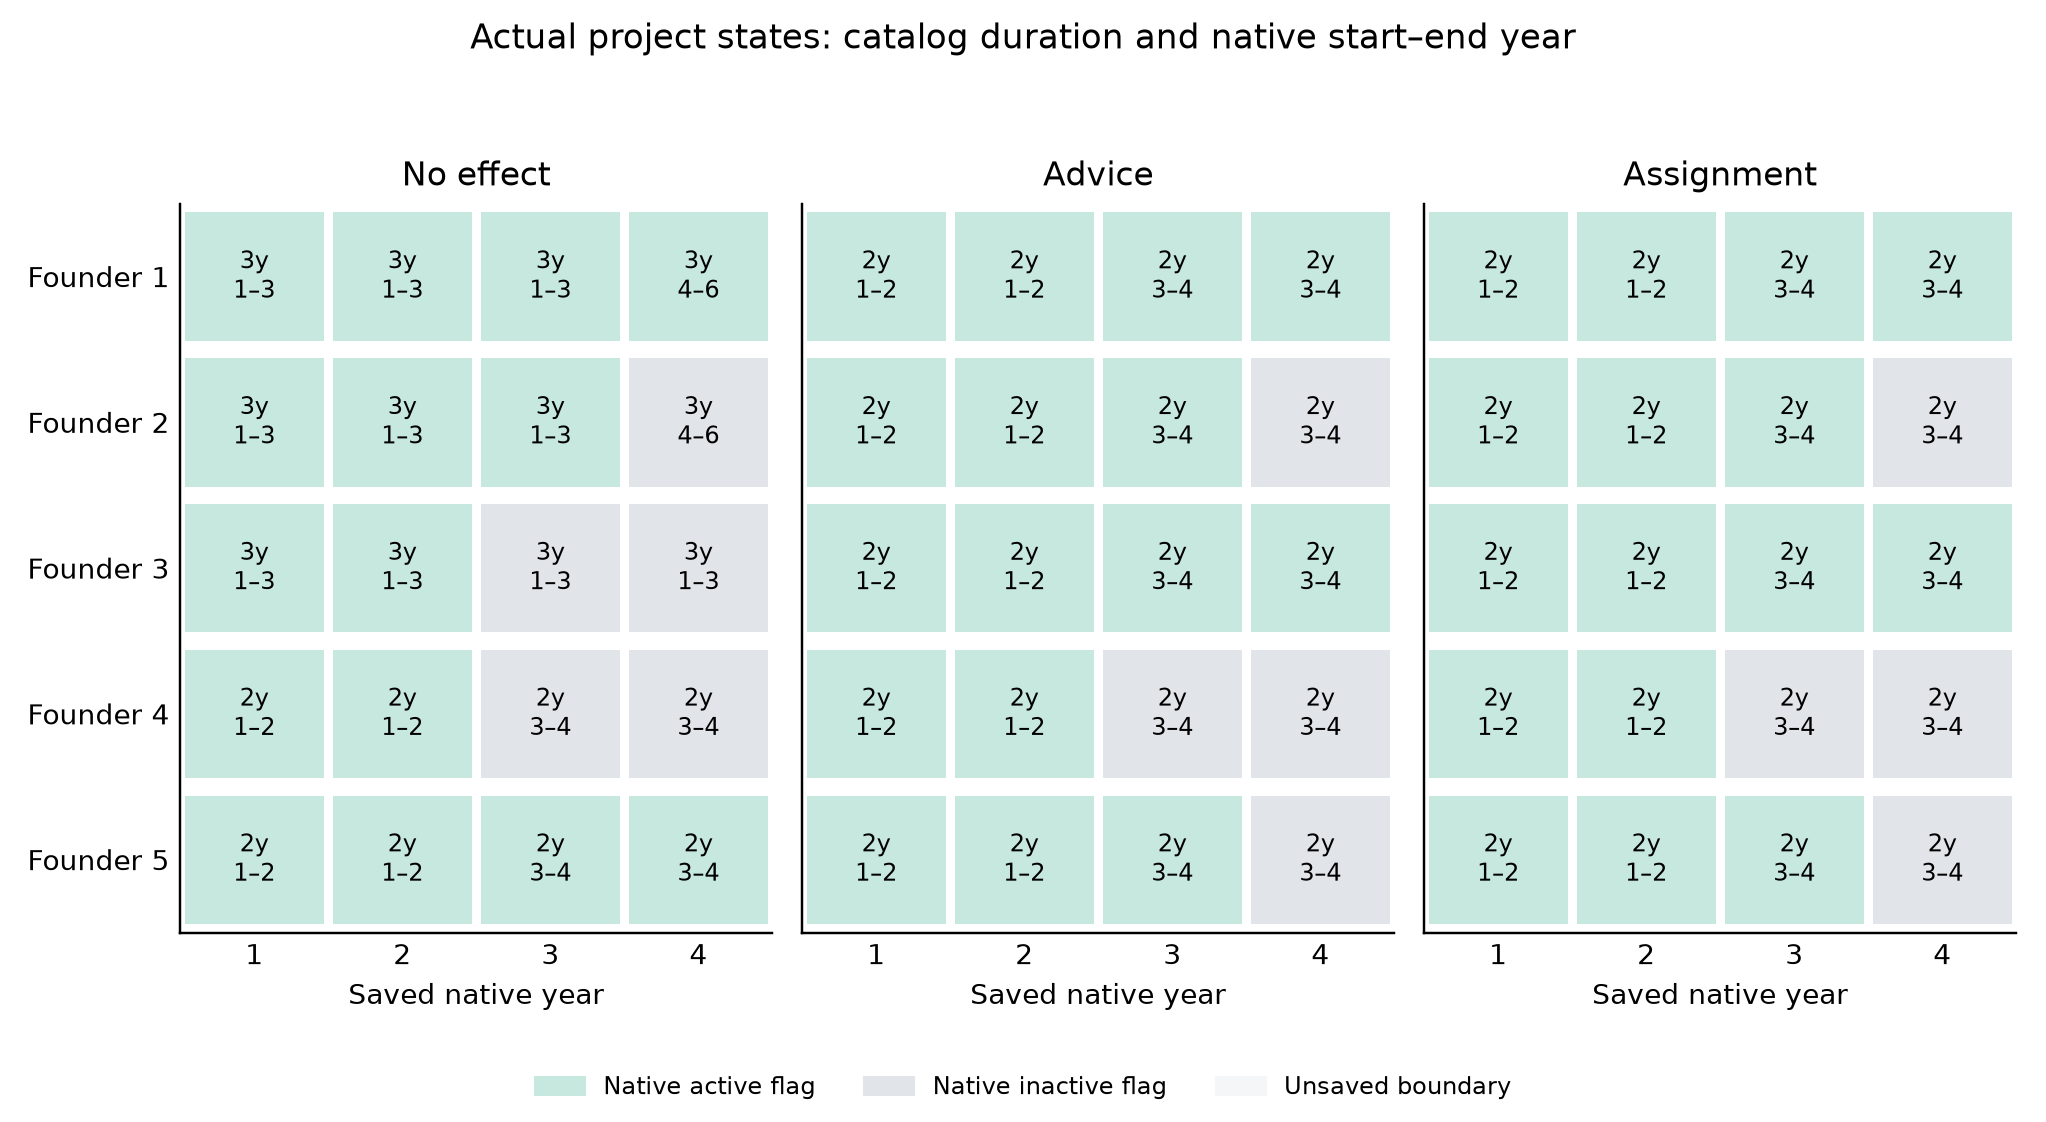
\includegraphics[width=\linewidth]{figures/native-catalog-actuation-v1/project-states.png}
\caption{Actual saved project states for all five founders and four years
in each arm. Cells show the catalog duration and native start--end years;
colors encode original active flags. Project dates and flags are different
quantities. The two-year effectful agenda contrasts with the initial mixed
two/three-year path, without changing original production laws.}
\label{fig:catalog-projects}
\end{figure}

The effectful arms each have 18 rather than 12 accepted decision records
and 16 rather than 15 active founder boundaries. Their annual active counts
are 5,5,4,2 versus 5,5,3,2 for no effect
(Figure~\ref{fig:catalog-losses}). All three end with two active founders.
Final total founder resources are 50,40,40 in the table's order, so this is
not an improvement in every reported quantity. Accepted decisions remain a
proxy, not verified discoveries; $P$ remains a native flag sum, not meaningful
work or continuous survival.

\begin{figure}[t]
\centering
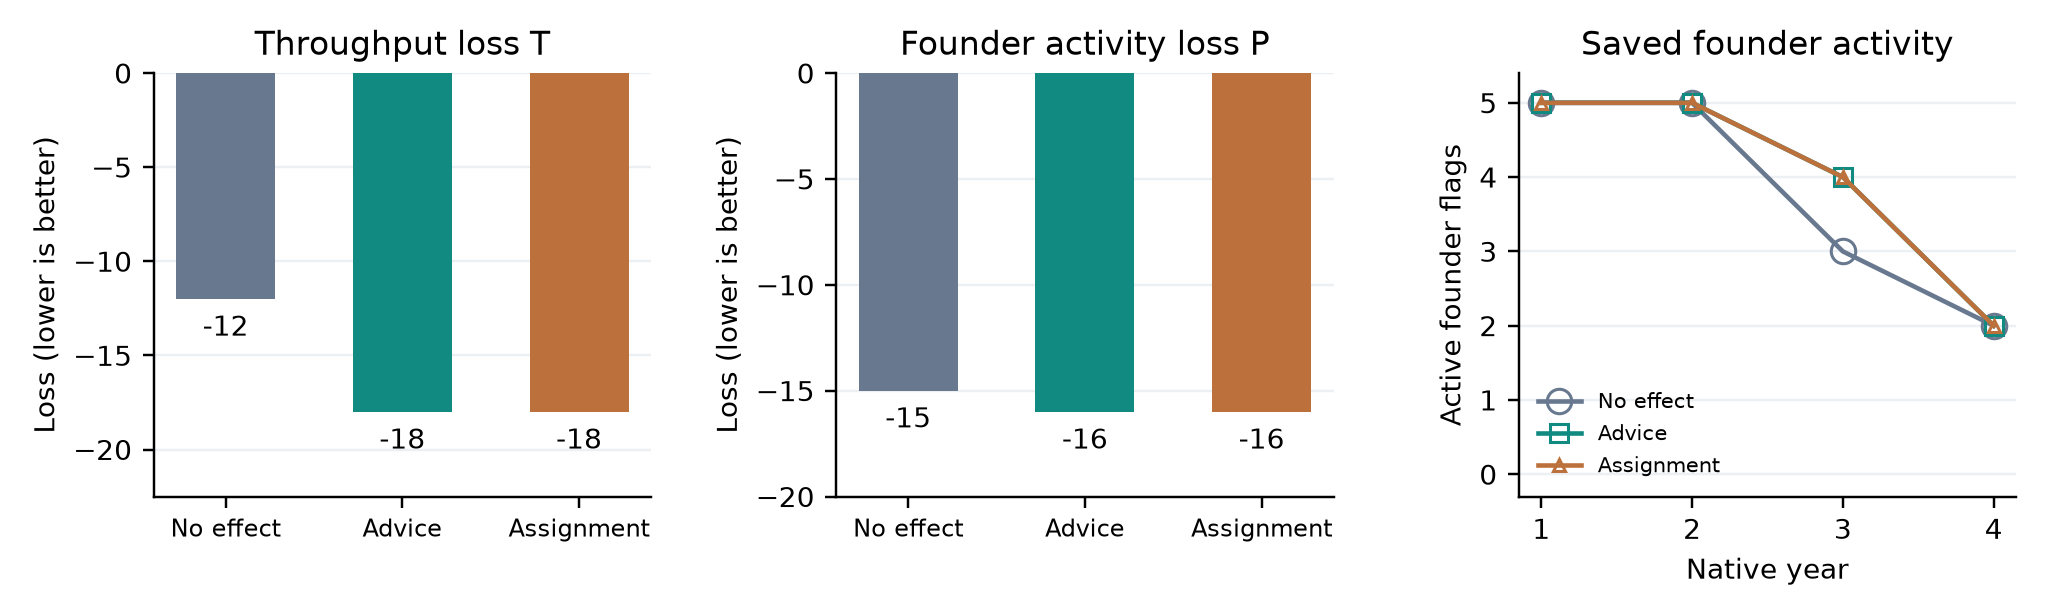
\includegraphics[width=\linewidth]{figures/native-catalog-actuation-v1/losses-and-activity.png}
\caption{Actual T/P losses and annual founder flags in all three completed
worlds. Advice and direct assignment tie both recorded losses despite distinct
request counts and full scientist-input histories. There is no observed
T/P trade-off in this comparison and no seed uncertainty estimate.}
\label{fig:catalog-losses}
\end{figure}

\subsection{Inference boundary and measured cost}
The comparison establishes an effective planning path available to an
institution, not autonomous invention or a demonstrated objective-to-system
distinction. Identical initial rules and permitted authority do not imply
identical later inputs. All three full ordered scientist-input sequences
differ, including the two equal-loss arms. Their later resource and model
response histories can evolve differently. Changed plans and accepted output
therefore do not isolate project duration as the sole mediator. The earlier
generic-advice null uses a different message and world scope; it is not a
matched message-granularity ablation of this study.

All 496 scientist requests have committed replies, with 518,946 reported
input tokens and 45,741 output tokens. The 90,562 cached prompt tokens are
a subset of input, not an additional charge. Three scientist-load POSTs have
unknown token usage. There are no designer-generation or critic POSTs.
Native execution takes 31min15s, followed by about 46s to original double
audit and cost closure. These are local observed wall times, not energy or
fresh-machine benchmarks.

This result supplies useful same-authority reference policies for subsequent
free planning/allocation search. A count/content study must still evaluate
its own actual submitted designs, both objectives and every strong reference,
then fix selections before unused-condition evaluation. A new graph is not
required; neither is a positive result. The new planning study is not counted
as complete here: its first initial-readiness attempt stops when the local
service receives a termination signal, before any reference or own candidate
world. A separately predeclared fresh attempt cannot erase that stop or its
unknown response costs. The completed three-arm evidence alone does not close
the important empirical question or justify a main-conference-ready judgment.
\FloatBarrier

\section{Discussion: what can be concluded across the program}
\subsection{The objective-to-system map is the research object}
The studies are not another survey of hand-selected acceptance or funding
settings. A loss enters a search procedure, which returns a specification and
a history; common evaluation then characterizes that returned system.
Parameter optimization exhibits two selected designs under three objectives.
Structural cases exercise different organizing algorithms. V2 shows that
strong simple rules can remove apparent gains against an editable seed.
The meaningful output is the conditional map from objective and permitted
design domain to generated mechanisms, paths, costs and consequences.

That map need not be injective: different objectives can select the same
institution. It need not be robust: a development winner can change rank on
unused conditions. It need not select a novel institution: all-accept or
reviewer-free reject may minimize a proxy. These are valid experimental
outcomes, but not automatically important general findings. A future paper
must substantiate which observed pattern extends beyond elementary incentives
and this particular designer/world combination.

\subsection{Expressivity, exercise and optimization must be measured separately}
The V8/V12 cases show that source-defined nodes, routes and plan processes can
execute; V13 shows observed free-code gains with an external author. The later
matched local study does not exercise declared topology changes at all.
These are compatible results with different provenance, not a contradiction
to be resolved by discarding the earlier cases or attributing them to the
local designer. The platform can support a behavior that a particular search
does not find within its finite budget.

Similarly, technical validity rates are scientifically relevant to end-to-end
optimization, but they confound any claim about intrinsic design-space value.
All local LLM numeric proposals failing while uniform numeric proposals
execute is evidence about the tested package. It is not proof that parameters
are intrinsically harder than code or that code/graph freedom is superior.
Future interface interventions should be prospective, not repairs/refills of
the V2 record.

\subsection{Gradients are an option, not an ontological requirement}
The most general target is free scientific-system optimization using available
evaluation and gradient information. Exact autograd is appropriate inside a
represented differentiable institution; response surrogates require native
fidelity checks; likelihood-ratio estimation can surround a discrete/opaque
world if its sampled design distribution is known. No universal differentiable
replacement of language, retrieval and science is required.

Our measurements do not show a practical estimator advantage. The V9 fitted
operator fails an unused finite-path check, V10's moving methods tie the known
incumbent, V11's updates do not discover a better first best, and neither V13
gradient followup improves its previous best. These observations should guide
better estimator targets and uncertainty accounting, not be hidden behind
the fact that a backward pass exists. They also do not prove all gradient
methods ineffective: targets, information and tiny budgets differ.

\subsection{From institutional revision to recursive improvement}
There are at least four different claims: a program is revised; the revised
program has a better observed loss; repeated revision improves expected
performance on new conditions; the revision procedure or inventor itself
becomes better. Our external-author cases sometimes support the second, and
local pipelines implement the first. They do not establish the third or fourth.
Scientist/designer weights are not trained here. A history-aware author is
not thereby a recursively self-improving optimizer.

A persistent society that changes its own organizing system is another axis.
It raises state migration, policy-selection bias and counterfactual evaluation
questions not answered by resetting worlds. Checkpointed designs, explicit
adoption and source-bound trajectories provide infrastructure, not a completed
recursive-improvement result. Keeping these levels explicit preserves the
long-term motivation without selling it as current evidence.

\section{Related work}
ScienceUtopia studies a persistent research ecosystem and institutional
interventions~\citep{jin2026scienceutopia}. Our design object is the executable
organizing system returned by a loss-conditioned search. This is a different
question, not a claim that the source world is realistic enough to validate
policy or that its reported large-model experiments are reproduced locally.
Science-of-science and research-assessment work motivate plural objectives
and skepticism about proxy optimization~\citep{fortunato2018science,hicks2015leiden}.

Optimization through generated programs is prior art. OPRO uses evaluated
solutions as feedback~\citep{yang2024opro}; ADAS searches code-defined agentic
workflows~\citep{hu2024adas}; AMD-LLM evolves mechanism code with problem-specific
fixing~\citep{liu2025mechanism}. Our no-host-repair contract is a comparison
choice, not a superiority claim. SGA combines LLM outer expression search with
continuous inner optimization~\citep{ma2024sga}. GPTSwarm optimizes agent-graph
connections with score-function methods~\citep{zhuge2024gptswarm}. Thus code
generation, graph search and mixing discrete design with gradients are not
first contributions here.

The AI Economist studies learned social policy~\citep{zheng2020economist}, and
LLM Economist adapts workers and a planner through context under bounded tax
actions~\citep{karten2025economist}. AgentSociety2 integrates composable
environments and specification-to-code~\citep{piao2026agentsociety2};
SocialSystemArena compares governance specifications~\citep{fei2026institutions};
PolicySim optimizes exposure actions in an LLM-based social
environment~\citep{huang2026policysim}. We focus on editable scientific
organization and its longitudinal native effects. Domain specificity alone
does not establish greater generality, scientific significance or priority.

Likelihood-ratio, reparameterization and control-variate methods are existing
theory~\citep{parmas2021unified,parmas2022proppo,parmas2023composite}.
Our contribution is the explicit placement and evaluation of these boundaries
in this design environment, not a new unbiased estimator for arbitrary
LLM-generated institutions.

\section{Limitations and responsible interpretation}
The native world is itself simplified. Literature retrieval stands in for
many real scientific activities; it does not conduct physical experiments,
verify novel knowledge or reproduce the full social organization of science.
Our extension preserves that world but does not eliminate its assumptions.
The native action registry is extensible, not an already implemented semantics
for every possible laboratory, government or hypothesis-testing institution.

Experiments are small and exploratory. Historical objectives and coefficients
are engineering choices informed by development, not preregistered hypotheses
about real science. The parameter study's five evaluation seeds and V2's five
unused seeds are small; their source/design spaces differ. Other cases share
one development seed, some use common-prefix replay, and external-author
provenance differs from local35B generation. These distinctions prevent pooled
causal method rankings or broad model generalization.

Review scores are endogenous LLM outputs, not truth. Better count, review
utility or resource snapshots do not validate scientific value, equity or
harm. Proxy-seeking institutions should be examined, not deployed by default.
No study of actual researchers, human intervention, independent truth verifier
or real scientific-policy deployment is reported.

Reproducibility has layers: numerical reconstruction from retained reports,
full raw/source re-audit, and fresh inference. The first is demonstrated for
V2, with explicit historical receipts for other studies; the latter is not
guaranteed by seeds. The local35B upstream revision/conversion recipe remains
unverified. Some usage is unknown and total project FLOPs, energy and monetary
cost are not measured. Appendix~\ref{app:reproduction} states these boundaries.

This manuscript uses a retained NeurIPS2025 preprint style for readability,
without a page cap; it is not compliance with a selected future conference
cycle. Human authorship/responsibility and public redistribution rights are
not finalized. Experimental LLM roles and AI assistance in implementation,
analysis, figures and prose must be disclosed, not represented as independent
human peer review. No actual submission, public upload, model replacement
or new experiment is performed by preparing this manuscript.

\section{Conclusion}
The system that organizes science can be an executable optimization object
containing the original persistent researcher world. Institution code,
mechanisms, connections and processes are not restricted to a menu of
acceptance/funding knobs, and black-box evaluation can coexist with scoped
gradient information without making the entire world differentiable.

The integrated evidence is mixed and informative: objective-conditioned
parameter selection yields uncertain trade-offs; structural programs can alter
real plans and information routes; external source redesign can improve an
observed proxy while gradient followups worsen; the matched local study
reveals compliance failures, no exercised topology search and no advantage
over strong simple references. A canonical game-like interface makes those
same successes, ties and failures inspectable.

The next scientific step is not scale alone. It is to identify a specific
organizing freedom whose native effect can be separated from interface burden
and elementary proxy incentives, then test it with a finite, fair comparison.
This manuscript preserves the full research program while distinguishing
implemented capability, exercised mechanism, observed optimization and the
stronger claims still requiring evidence.

\FloatBarrier
\clearpage
\phantomsection
\addcontentsline{toc}{section}{References}
\begingroup
\setlength{\bibsep}{3pt plus 1pt minus 1pt}
\bibliographystyle{plainnat}
\bibliography{references,submission-sources}
\endgroup
\clearpage
\appendix
\section{Complete parameter-study context}
\label{app:parameter}
The fixed-topology study and V2 use different sources, horizons, design spaces
and losses. They are retained because they answer different questions, not
combined into one leaderboard. Table~\ref{tab:integrated-parameter-designs}
shows both distinct designs, rather than imply that three objective names
produce three different institutions.

\begin{table}[ht]\centering\small
\caption{Full frozen parameter settings. Topic and burden independently select
the right-hand design. Funding application cost is fixed at 1 in both.}
\label{tab:integrated-parameter-designs}
\begin{tabular}{lrr}\toprule
Parameter & Participation-selected & Topic/burden-selected\\\midrule
Acceptance rate & .496777 & .113159\\
Funding application cost &1&1\\
Funding slot fraction &.390677&.327413\\
Resubmission cost &12.8905&16.3863\\
Review policy &persona&standardized\\
Reviewer capacity &8&2\\
Reviewer matching &topic&random\\
Reviews per paper &3&4\\\bottomrule
\end{tabular}\end{table}

The retained intervals are exact nonparametric percentile bootstrap intervals
for the complete LossSpec aggregate over the five declared evaluation seeds.
They are not confidence guarantees for a different source or a broader model
population. All nine paired loss-contrast intervals include zero. Two labels
share a design but have separate stochastic held-out trajectories; comparing
them as if they were distinct institutions would exaggerate diversity.

\begin{figure}[p]\centering
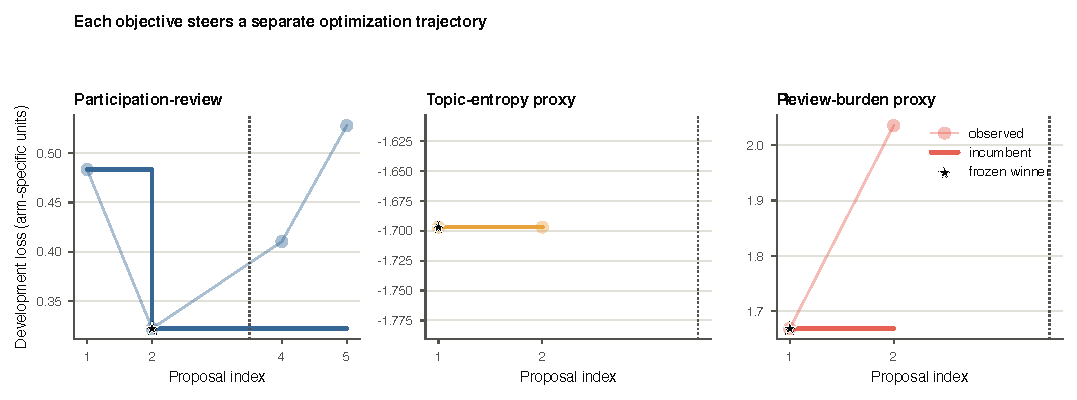
\includegraphics[width=\linewidth,height=.78\textheight,keepaspectratio]{generated/metric-conditioned/figures/metric-conditioned-objective-trajectories.pdf}
\caption{\textbf{Complete parameter-study development paths.} Three fixed
objectives, five candidates per arm and common development conditions.
Technical nulls do not become numeric penalties. Stars are frozen selections;
these are not additional held-out results or an optimizer comparison.}
\label{fig:integrated-parameter-paths}
\end{figure}

Declared gaming flags in that study are diagnostic alerts, not invalidity or
adoption vetoes. They do not override the loss. Recorded attempt runtime is
at least 52.35 h across that historical study, with one interrupted attempt's
wall time unknown; it is neither the later V2 runtime nor new compute for
this integrated manuscript. Logical rows, physical executions, adopted
trajectories and retries remain separate in the original paper slice.

\section{Complete structural case tables and interpretation}
\label{app:structural}
\begin{table}[h]\centering\small
\caption{All eight V8 structural-case outcomes. Graph is nodes/edges.
$U=3.25A-Q+0.05R$ differs from V2's $C$. Each row is a development execution;
cross-scores reuse its checkpoint. Values are display-rounded only.}
\label{tab:integrated-v8-all}
\begin{tabular}{llrrrrrr}\toprule
Arm & Generation/draw & Graph & $A$ & $Q$ & $R$ & $T$ & $U$\\\midrule
Throughput&G0/0&16/22&9&29&27&-9&1.6000\\
&G0/1&16/22&9&29&27&-9&1.6000\\
&G1/0&17/24&10&31.3333&30&-10&2.6667\\
&G1/1&16/22&10&33.6667&30&-10&.3333\\\addlinespace
Utility&G0/0&16/22&0&0&0&0&0\\
&G0/1&16/22&0&0&0&0&0\\
&G1/0&18/24&1&3.6667&18&-1&.4833\\
&G1/1&18/24&1&3.6667&18&-1&.4833\\\bottomrule
\end{tabular}\end{table}

An initial V8 authoring attempt fails before native inference because its
parent normalization does not match the exact saved request. That zero-world
failure remains in provenance, not as a fabricated scientific loss or a
successful attempt. The separately declared corrected-file workflow does not
replace an unsuccessful native trajectory. External authors may inspect their
own source and traces, richer information than a scalar-only oracle.

\begin{table}[h]\centering\small
\caption{All six V12 free-redesign observations, including the worse clinic
revision and return to its actual incumbent parent. Repetition is not new
invention; $Q$ uses original review means.}
\label{tab:integrated-v12-all}
\begin{tabular}{llrrrrrr}\toprule
Arm & Generation & Graph & $A$ & $Q$ & $R$ & $T$ & $U$\\\midrule
Throughput&G0&17/25&10&$95/3$&30&-10&$7/3$\\
&G1&17/25&10&$95/3$&30&-10&$7/3$\\
&G2&17/25&10&$95/3$&30&-10&$7/3$\\\addlinespace
Utility&G0&16/22&3&$32/3$&15&-3&$-1/6$\\
&G1&17/24&1&4&15&-1&0\\
&G2&16/22&3&$32/3$&15&-3&$-1/6$\\\bottomrule
\end{tabular}\end{table}

In V12, 32 source/context/result executions join committed native events;
throughput's10 amendments per world match generated outputs and annual
project state. Utility G1 emits two year 1 amendments and no additional year 2
clinic amendment. The historical code ABI does not retain a fully bound
upstream plan, so a stronger complete applied-plan hash cannot be reconstructed
for that slice. V13 prospectively records the full upstream plan and ordered
commands, enabling the stronger join. Later provenance improvements do not
retroactively repair old records.

For V13, actual eligible reviewer identities pass through a typed routing
capability to the original review prompt/model/parser. The source chooses a
subset of tasks, including none; the host does not choose favorable scores.
Original eligibility/COI and identity legality remain explicit native semantics.
A zero-review rule must author its own compatible selection consumer. The
new G1 ranking uses prior reviews to predict task desirability, not to replace
actual reviewer evidence in the measurement.

\FloatBarrier
\section{Gradient assumptions, diagnostics and complete followups}
\label{app:gradient}
\subsection{What each derivative covers}
For a categorical choice with logits $\alpha $, the sampled score is the
one-hot choice minus its probability vector. For a Gaussian latent with mean
$\mu $ and fixed scale $\sigma $, the mean score is $(z-\mu)/\sigma^2$.
These derivatives concern the retained sampling law. A fixed sigmoid mapping
the latent to a bounded cutoff does not require a native world derivative in
the LR estimator. Replacing the sampling law, truncating its support without
accounting, or changing source semantics changes the estimator's target.

Leave-one-out baselines rely on conditional independence of the other design
draws; they are not a license to reuse arbitrary correlated outcomes as a
baseline. Controls in Eq.~\eqref{eq:integrated-control} are fixed from eligible
prior history for the current scored batch. Their expectation correction
must be computed for the same distribution. If the world's conditional law
depends on $\theta $ beyond the sampled executable design, the stated simple
score identity is incomplete. Missing technical outcomes and adaptively
selected histories require their own estimand analysis.

The local response representation takes a different route: it approximates
sensitivities inside the native path. A faithful hard replay verifies value
accounting, not the correctness of its soft derivative. A parameter disconnected
inside the explicitly represented subgraph can have derivative zero there;
unknown external researcher/host responses must remain unknown. Neither LR
nor the response operator differentiates arbitrary LLM source invention.

\begin{table}[h]\centering\small
\caption{All V9 coupled-history endpoints. C: calibration; U: unused coordinate;
G: frozen gradient proposal. The proposal at .50 is an exact no-op at stored
precision. The better observed .80 is not substituted for it.}
\label{tab:integrated-v9-all}
\begin{tabular}{lrrrrrr}\toprule
Role &$\theta $&$A$&$Q$&$R$&Native $U$&Predicted $U$\\\midrule
C0&.20&0&0&18&.9000&.9000\\
C1&.50&0&0&18&.9000&.9000\\
C2&.80&1&$10/3$&18&.8167&.8167\\
U0&.35&0&0&18&.9000&.9000\\
U1&.65&0&0&18&.9000&.8168\\
G&.50&0&0&18&.9000&.9000\\\bottomrule
\end{tabular}\end{table}

\begin{figure}[p]\centering
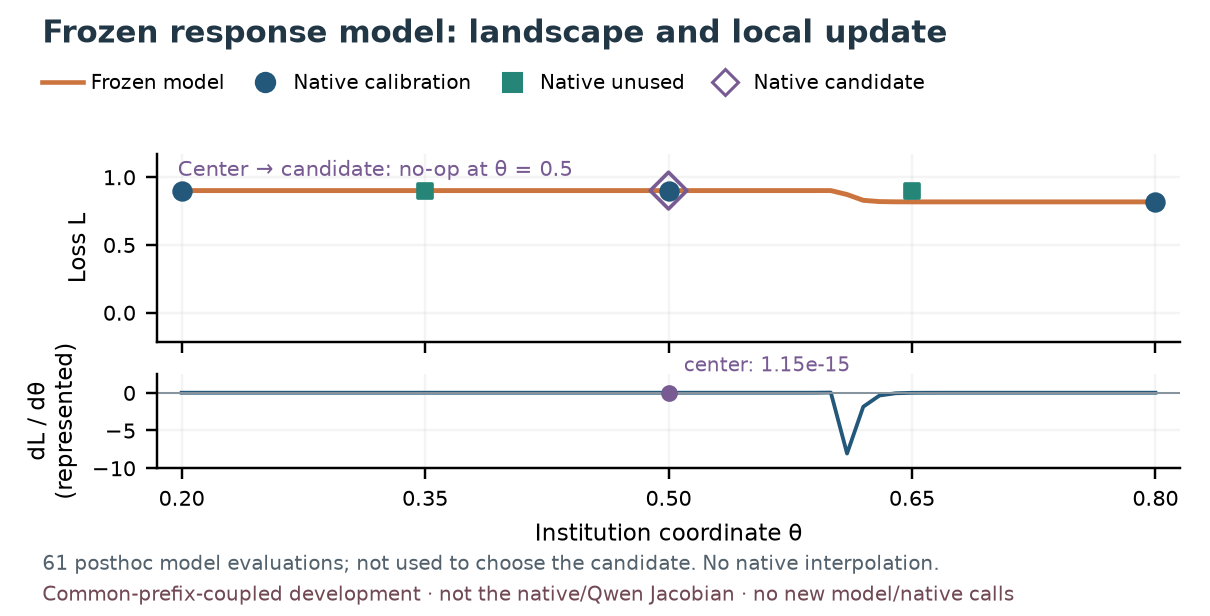
\includegraphics[width=\linewidth,height=.78\textheight,keepaspectratio]{figures/native-qwen-response-v9-a3-landscape.png}
\caption{\textbf{Frozen represented landscape and actual native endpoints.}
The plotted model evaluations are offline diagnostics, not new Qwen calls.
Calibration fit does not imply unused-coordinate or finite-path fidelity.
The precommitted gradient candidate remains the center rather than the known
lower calibration endpoint.}
\label{fig:integrated-response-landscape}
\end{figure}

\begin{table}[h]\centering\small
\caption{Offline temperature diagnosis at $\theta=.5$ on the same historical
calibration data. These are not four native experiments or prospective
temperature selection using future success.}
\label{tab:integrated-temperature}
\begin{tabular}{rrr}\toprule
Temperature & Center represented derivative & Calibration-loss RMSE\\\midrule
1&$-.24092$&.52717\\
.2&$-.09426$&.32974\\
.05&$+.01156$&.01522\\
.01&$1.15\times 10^{-15}$&$1.16\times 10^{-5}$\\\bottomrule
\end{tabular}\end{table}

The V10 gradient steps use a fixed temperature schedule $(1,.2,.05)$ and
$\theta_{k+1}=\operatorname{clip}_{[.2,.8]}[\theta_k+
\operatorname{clip}_{[-.1,.1]}(-.5\widehat g_k)]$.
They refit on only the three shared calibration endpoints and their own earlier
completed endpoints. The black-box policy instead refines the widest interval
adjacent to its observed incumbent, choosing the lower interval on ties.
Each arm's new losses are $(.9, 49/60, 49/60)$; neither beats the shared historical
best. Their six forwards contain 504 logical replies, 318 prefix replays and 186
new calls; support from shared historical calibration is counted once, not once
per method or as six independent societies.

\subsection{Score/control measurements and the previously missing forward}
V11's two arms each have four native losses $(.7833333, 1.2, 1.2, 1.2)$.
The first draw has $A=1,Q=11/3,R=24$; each remaining draw has $A=Q=0,R=24$.
The G0 score step changes Gaussian mean from 0 to $-.0407768$ and logits to
$[-.0495833,.0495833]$ before G1. The final prior-control estimate has mean
gradient $.742395$ and logit gradient $[.109754,-.109754]$; plain LR on the same
batch gives $.945250$ and $[-.570274,.570274]$. These single noisy estimates
are not empirical variance measurements.

The saved final mean $-.1150163$ and logits $[-.0605587,.0605587]$ are not
reevaluated within V11. Table~\ref{tab:integrated-control-forward} records the
separate complete two-world followup, not a retroactive extra V11 generation.
Historical outcomes are provenance, not a randomized concurrent control.

\begin{table}[h]\centering\small
\caption{Complete fresh followup of the exact saved V11 proposal. The bounded
executable cutoff differs from its Gaussian latent. Lower is better under the
same $U$, but two draws do not estimate comparative expected improvement.}
\label{tab:integrated-control-forward}
\begin{tabular}{lrrrrrr}\toprule
Aggregation&Cutoff&$A$&$Q$&$R$&$U$&Fresh replies\\\midrule
Minimum&3.549508&0&0&21&1.05&91\\
Mean&3.080488&2&7&21&.55&89\\\bottomrule
\end{tabular}\end{table}

\FloatBarrier
\section{V2 all-candidate cross-scores and failure accounting}
\label{app:failures}
The two matrices retain all 60 scheduled rows per primary objective, including
three histories and four generations for each method. G/X marks denote
generation/execution nulls, not zeros. Full-precision values, raw metric
components and missingness remain in the numerical JSON/CSV; display rounding
never affects selection. Loss scales are independent and not combined.

\begin{figure}[p]\centering
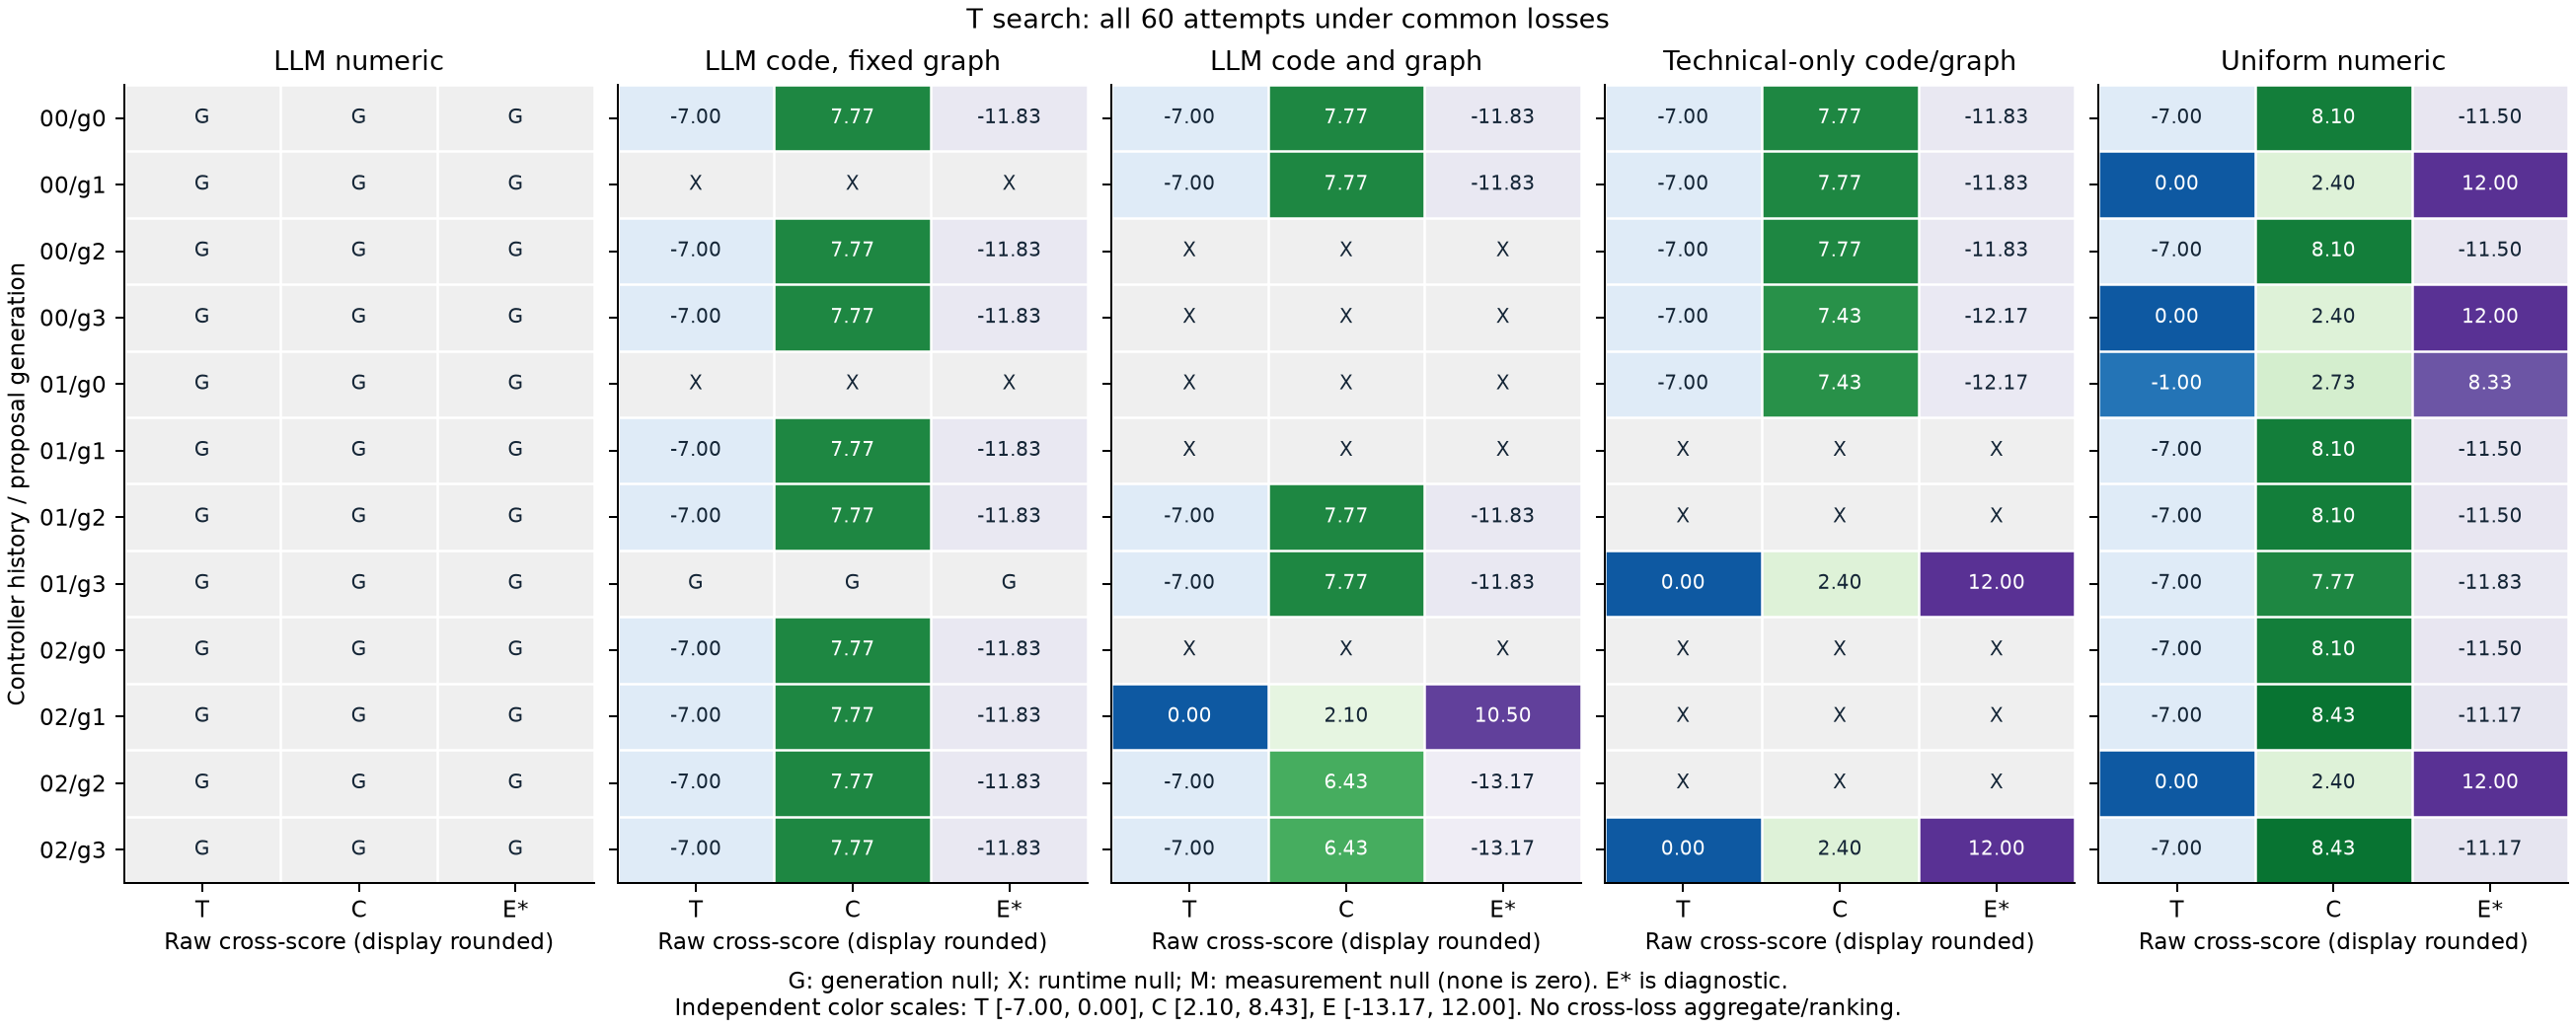
\includegraphics[width=\linewidth,height=.79\textheight,keepaspectratio]{generated/native-design-v2-supplement/all-cross-scores-throughput.png}
\caption{\textbf{Every V2 throughput-arm attempt under T/C/E.} These are
development cross-scores, not E-optimized selections or extra worlds. A favorable
E observation in a T arm is not relabeled an E-search result.}
\label{fig:integrated-all-t}
\end{figure}
\begin{figure}[p]\centering
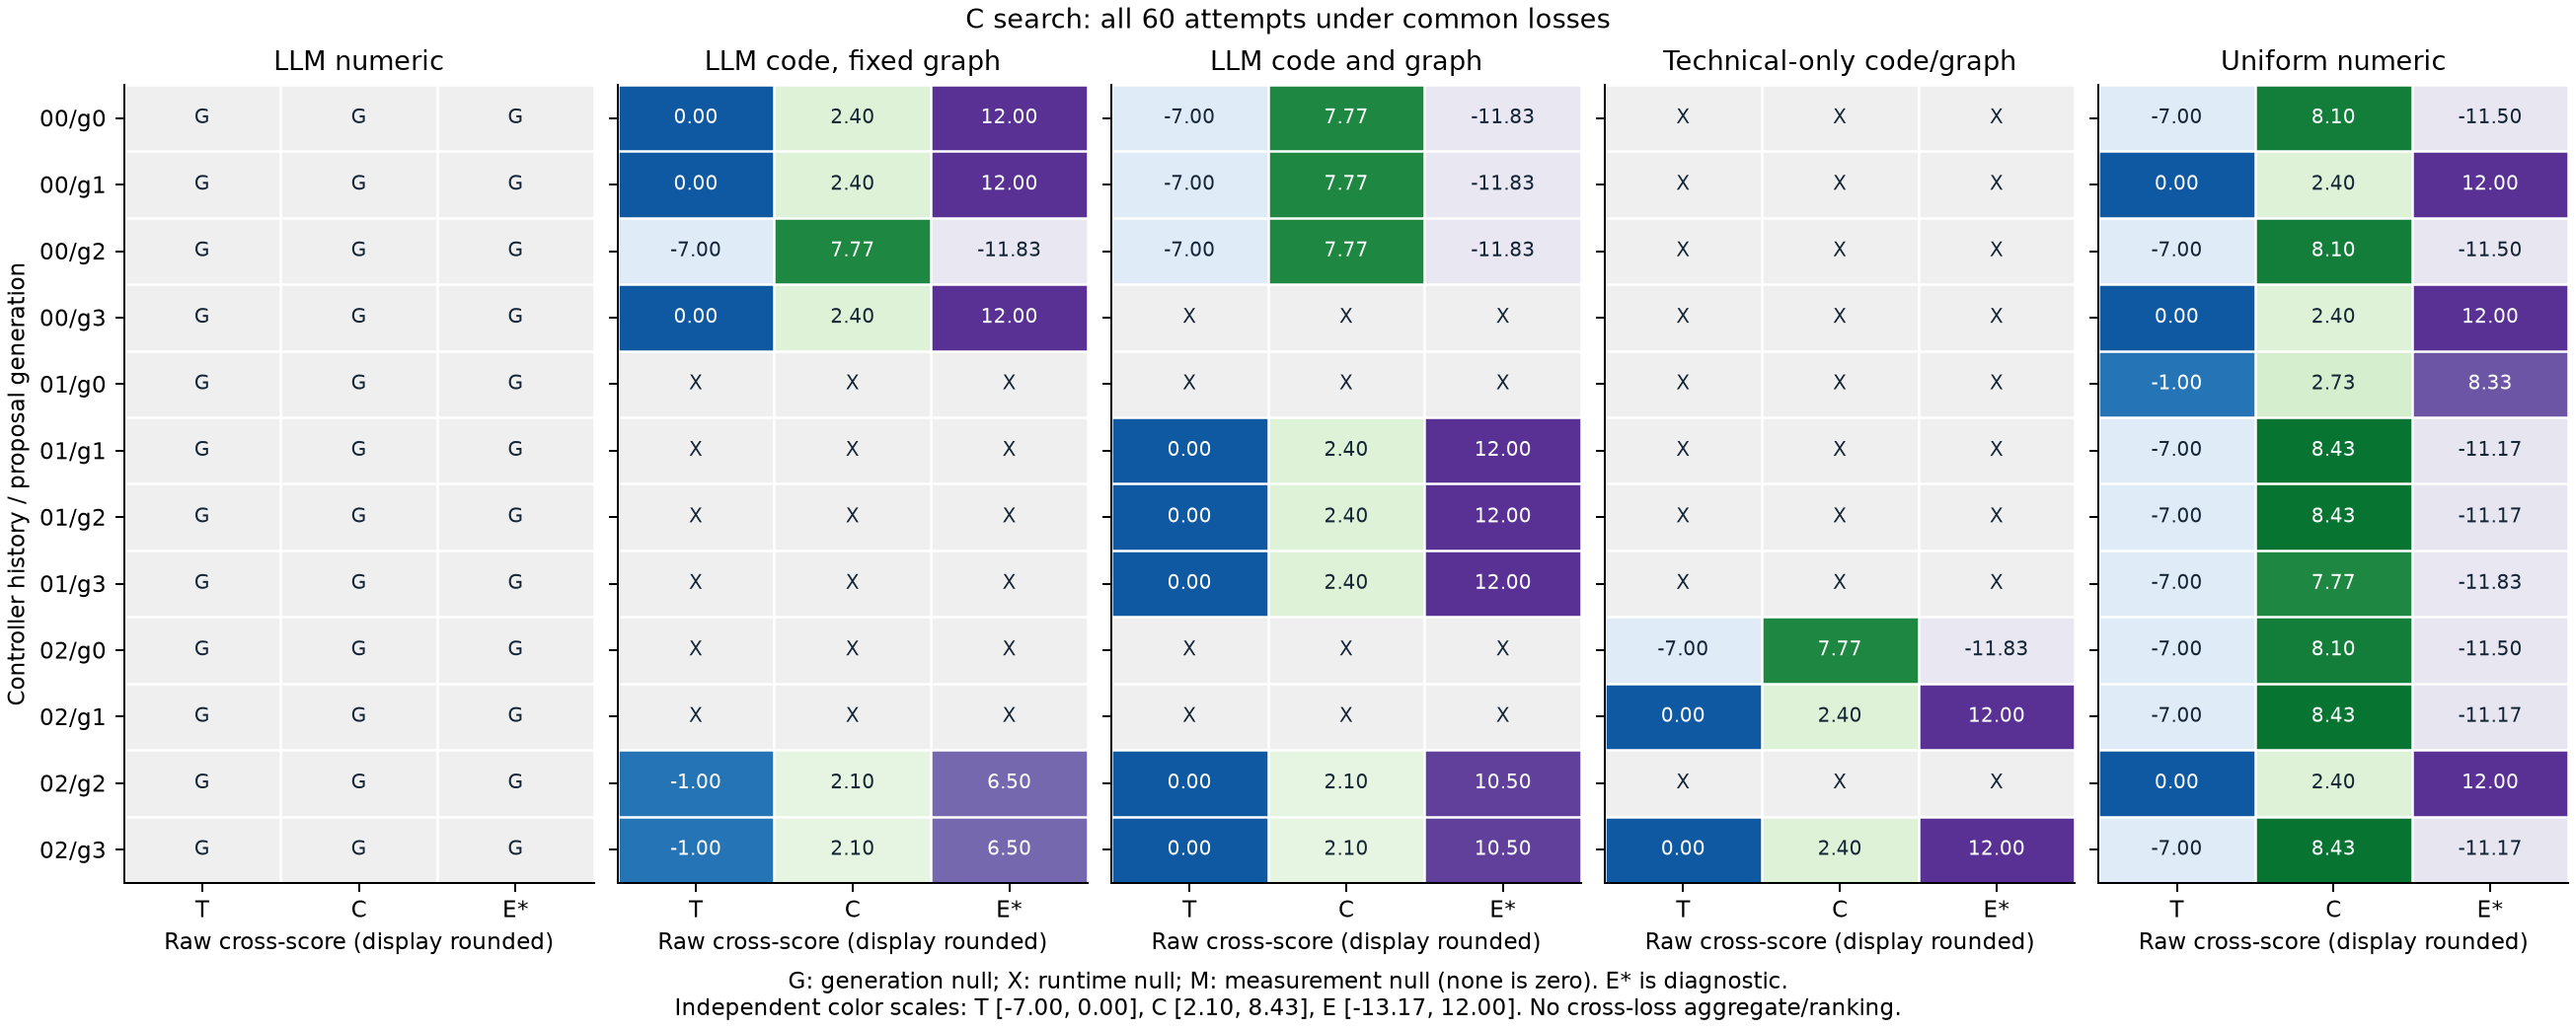
\includegraphics[width=\linewidth,height=.79\textheight,keepaspectratio]{generated/native-design-v2-supplement/all-cross-scores-selective.png}
\caption{\textbf{Every V2 C-arm attempt under T/C/E.} All failed attempts,
initial selections, ties and worse generations remain; there is no best-run-only
or successful-proposal-only reporting.}
\label{fig:integrated-all-c}
\end{figure}

The 31 execution failures comprise scalar-shape misuse 12, world-envelope errors 7,
decision-identity coverage 6, missing outputs 4, an extra output 1 and invalid
decision/score/reference 1. These are literal observed categories, not isolated
causes of designer cognition. The 25 generation-null slots exhaust the declared
action budget without valid explicit finish. A final provider envelope or
HTTP 200 is not necessarily a submitted executable institution.

The distinction between permission and use is also numerical: 40 of 64 completed
specifications change selection source; existing parameter-change row counts
overlap (bias 26, memory cost 24, threshold array 25, process count 20, router
threshold 24). No declared node/wiring/ABI/state/schedule changes are observed.
String/source identity, AST identity and arbitrary-input behavioral equivalence
are separate notions, none a hidden novelty gate.

\section{V2 costs, resources and separate longer horizon}
\label{app:costs}
\begin{table}[h]\centering\small
\caption{Search-only V2 components, pooled across three four-slot histories.
Designer seconds are host model-call time, not end-to-end wall or total compute.
Scientist replies include partial worlds. Zero author calls in uniform sampling
does not make native evaluation free.}
\label{tab:integrated-method-costs}
\begin{tabular}{llrrrrr}\toprule
Loss&Method&Complete/12&Author calls&Author s&Scientist replies&World dirs\\\midrule
T&Numeric LLM&0&192&2497.2&0&0\\
T&Code/fixed&9&172&2219.1&859&11\\
T&Code/graph&7&168&2413.4&739&12\\
T&Technical-only&7&168&2318.9&745&12\\
T&Uniform&12&0&0.0&1097&12\\\addlinespace
C&Numeric LLM&0&192&2580.9&0&0\\
C&Code/fixed&6&168&2519.7&682&12\\
C&Code/graph&8&167&2770.8&826&12\\
C&Technical-only&3&160&2361.9&459&12\\
C&Uniform&12&0&0.0&1107&12\\\bottomrule
\end{tabular}\end{table}

Search records 6514 scientist replies and 640 institution-code executions. Its 95
world directories, plus 9 fresh references and 90 physical evaluations, yield 194
response journals, not 194 completed forwards: completed forwards total 163.
Generation-null slots never dispatch a world. Proposal requests 1387 have 1385
final signals; validity/submission is checked separately.

\begin{table}[h]\centering\small
\caption{Measured V2 response-token scopes. Cached input counts are subsets,
not extra tokens. Model-load usage and total-project compute remain unknown.}
\label{tab:integrated-tokens}
\begin{tabular}{lrrrr}\toprule
Scope&Responses&Input&Cached input subset&Output\\\midrule
Scientists incl. partial worlds&16043&15547758&2976386&1473665\\
Designer proposals&1387&25969867&3102175&267057\\
Designer calibration&84&808832&22464&3819\\\bottomrule
\end{tabular}\end{table}

The 1764 auxiliary intents comprise 1387 proposal, 84 calibration and 293 role-load
intents. Loads separate 99 designer and 194 scientist contexts; their native
tokens are unreported, not zero. Native/provider/host durations overlap and
cannot be summed as project wall time. Overall writer wall is known, but exact
end-to-end per-trial wall allocation is not reconstructed from component data.
Retrieval, container orchestration, model loading, prior development and this
coding assistant's compute are not a measured project FLOP/energy/money total.

\begin{figure}[p]\centering
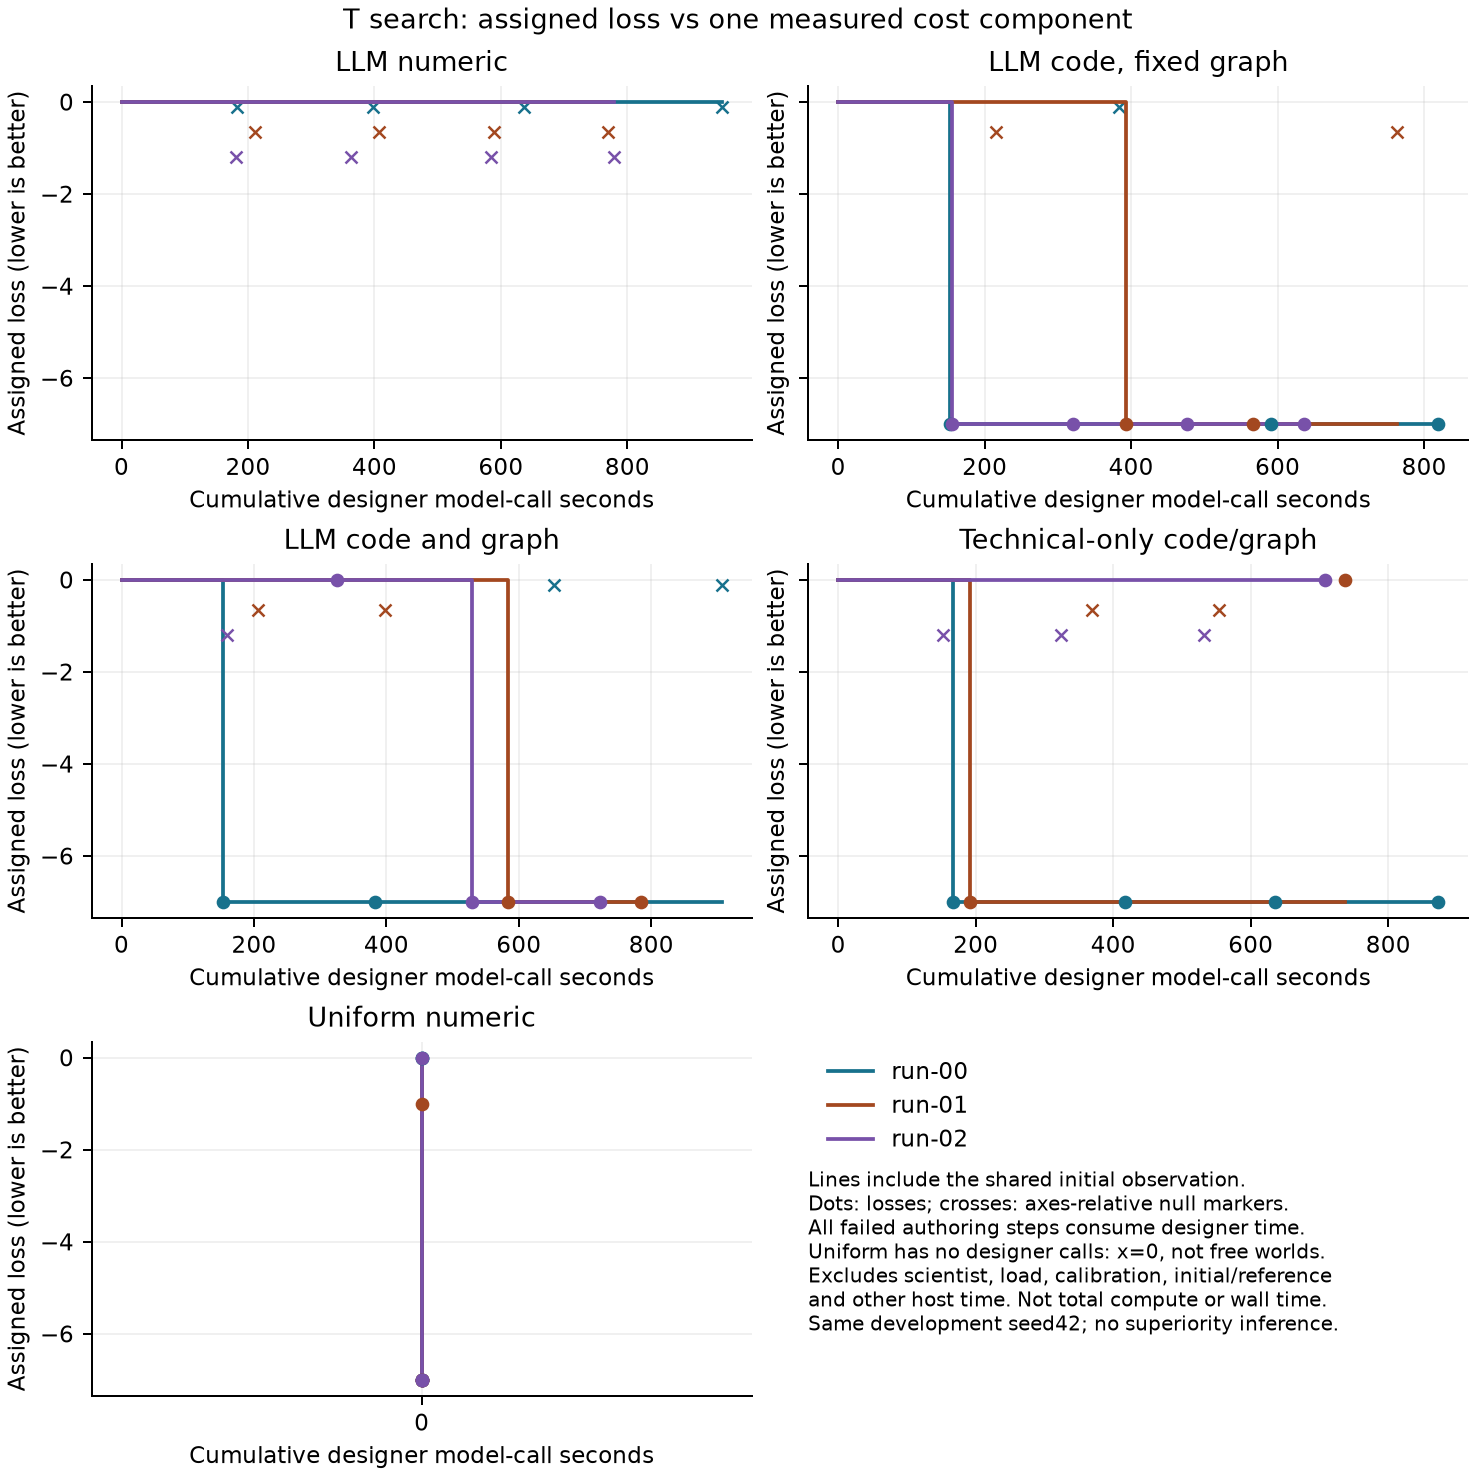
\includegraphics[width=\linewidth,height=.79\textheight,keepaspectratio]{generated/native-design-v2-supplement/designer-cost-paths-throughput.png}
\caption{\textbf{V2 T paths against cumulative designer host model-call time.}
All failed author steps are charged. Uniform is at zero designer time, not zero
world cost. Shared initial observations/calibration have separate excluded
costs; this axis is a measured component, not equal-compute superiority.}
\end{figure}
\begin{figure}[p]\centering
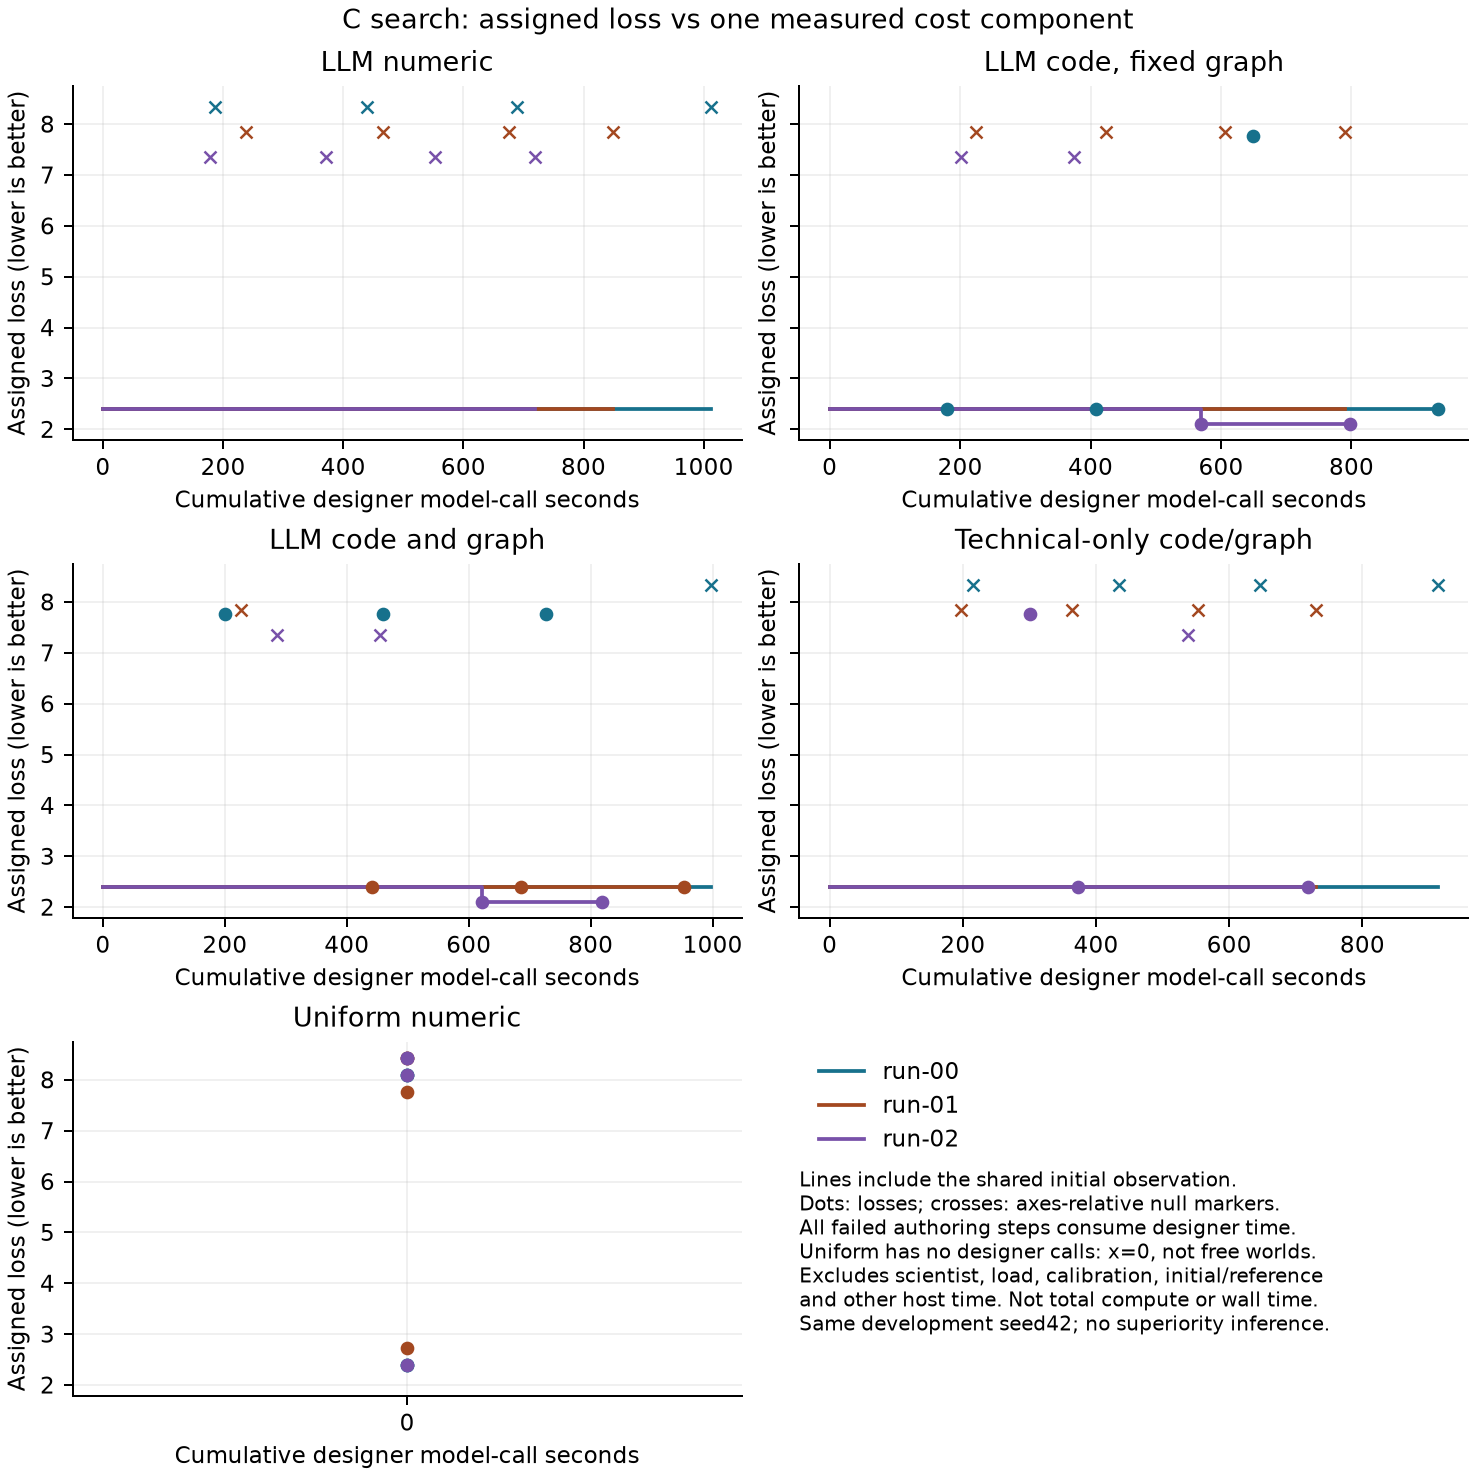
\includegraphics[width=\linewidth,height=.79\textheight,keepaspectratio]{generated/native-design-v2-supplement/designer-cost-paths-selective.png}
\caption{\textbf{V2 C paths against the same measured cost component.}
Three histories are shown without treating them as independent environments.
Missing component times would stop the cumulative axis, not be imputed as 0.}
\end{figure}

Outside metrics retain accepted decisions, original accepted peer-score sum,
review records, final original active authors, final author resources,
unreviewed acceptances, rejections and institutional-context deliveries.
Two-year resource means/ranges include initial 616(585--630),C code 627(595--640)
and T uniform 632(620--640). Descriptive overlap is not an equivalence test;
differences are not isolated causal benefits. Four-year initial 720,C code 780
and T uniform 760 remain single observations.

\begin{figure}[p]\centering
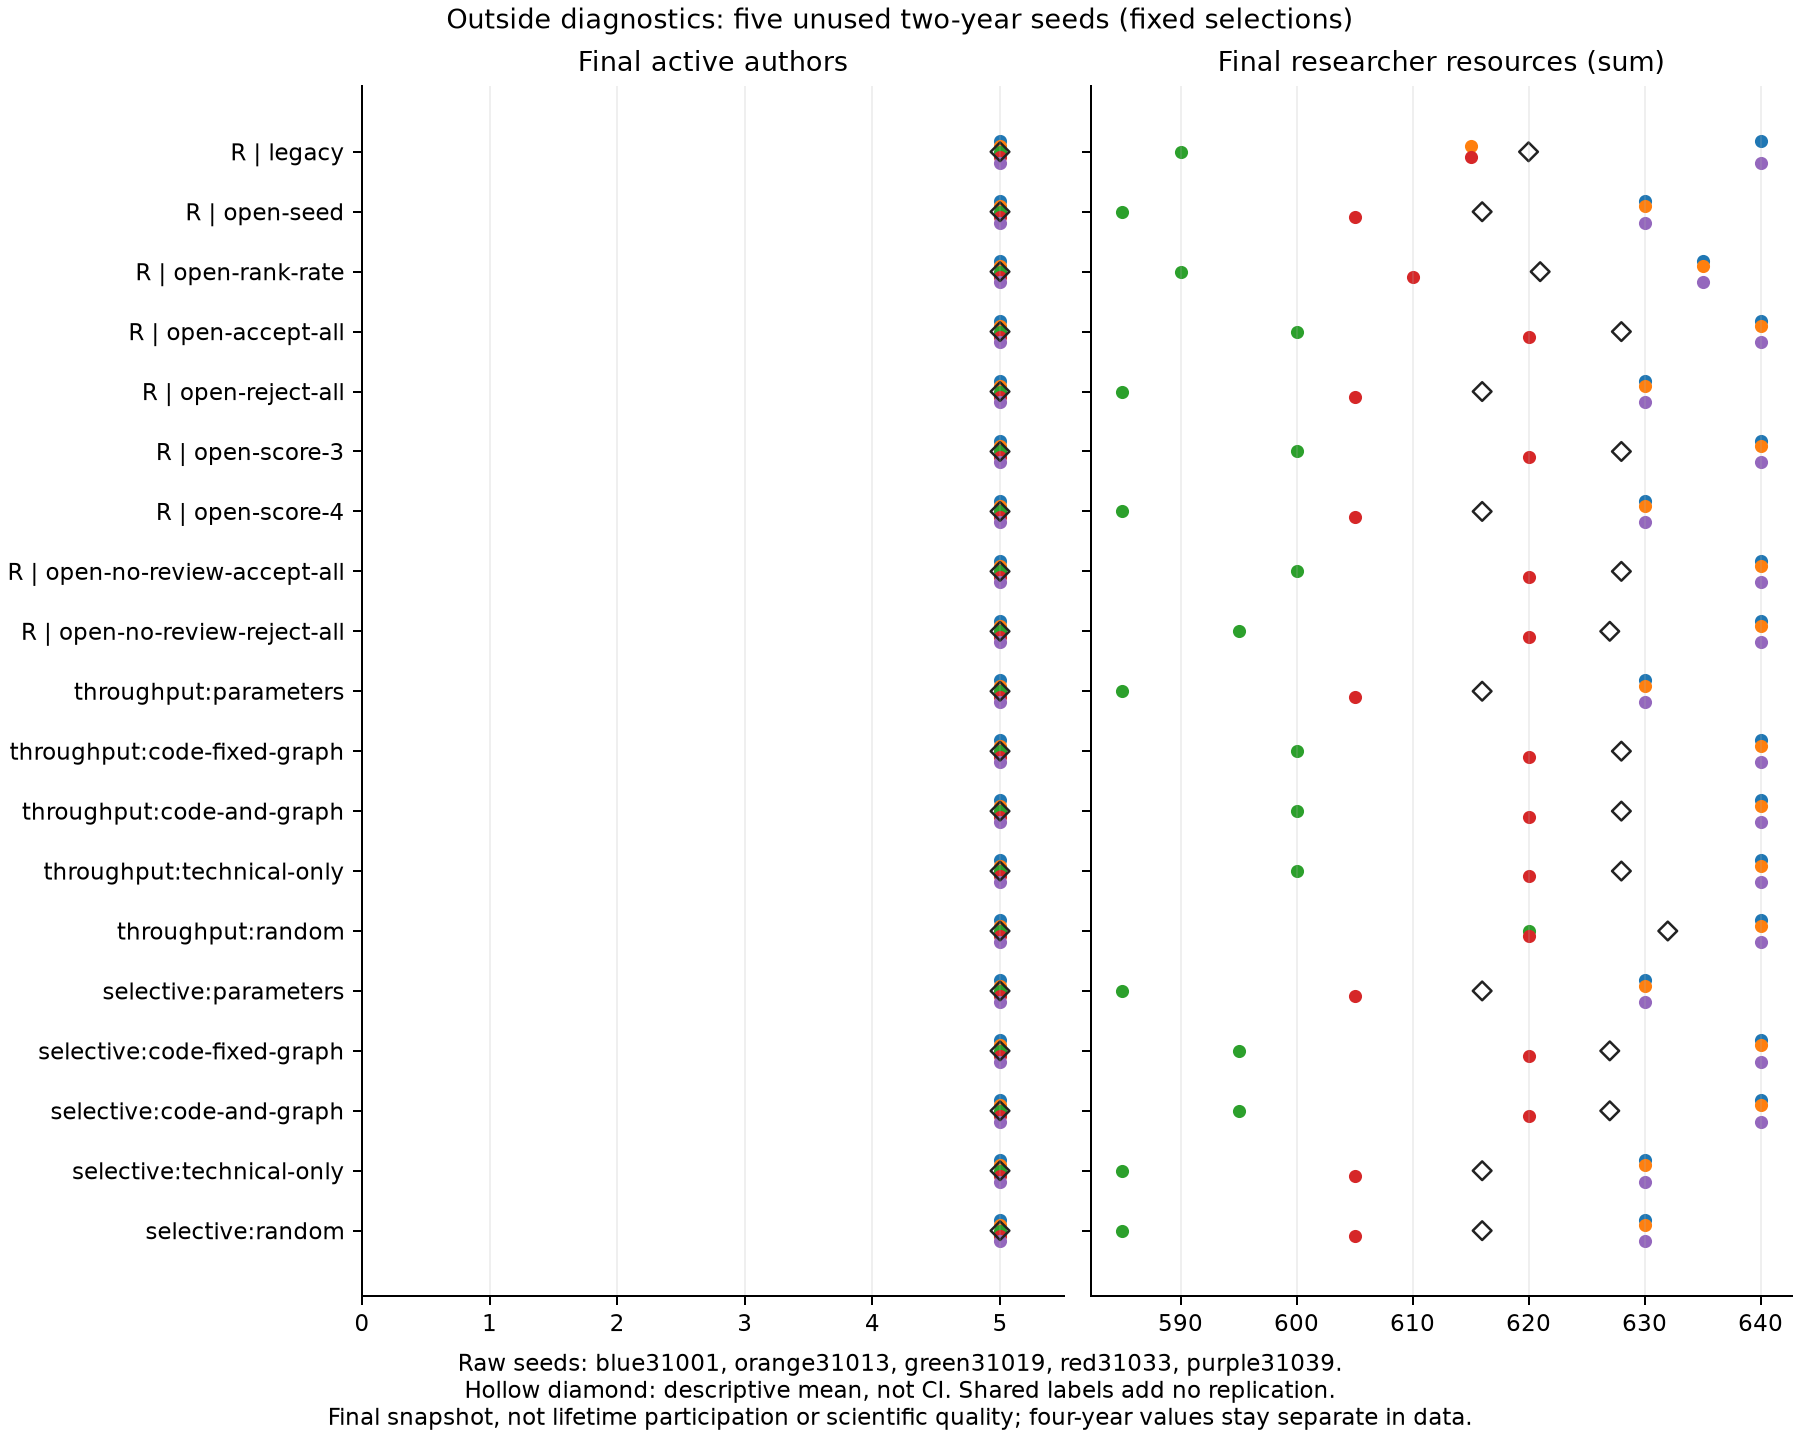
\includegraphics[width=\linewidth,height=.79\textheight,keepaspectratio]{generated/native-design-v2-supplement/outside-activity-resources-2y.png}
\caption{\textbf{V2 outside activity/resources on all selected/reference labels.}
The full 0--5 activity axis shows no final active-author separation. Five points
and descriptive means retain shared-policy identities. Native resources are
not money, welfare, scientific truth or an additional selection constraint.}
\end{figure}
\begin{figure}[p]\centering
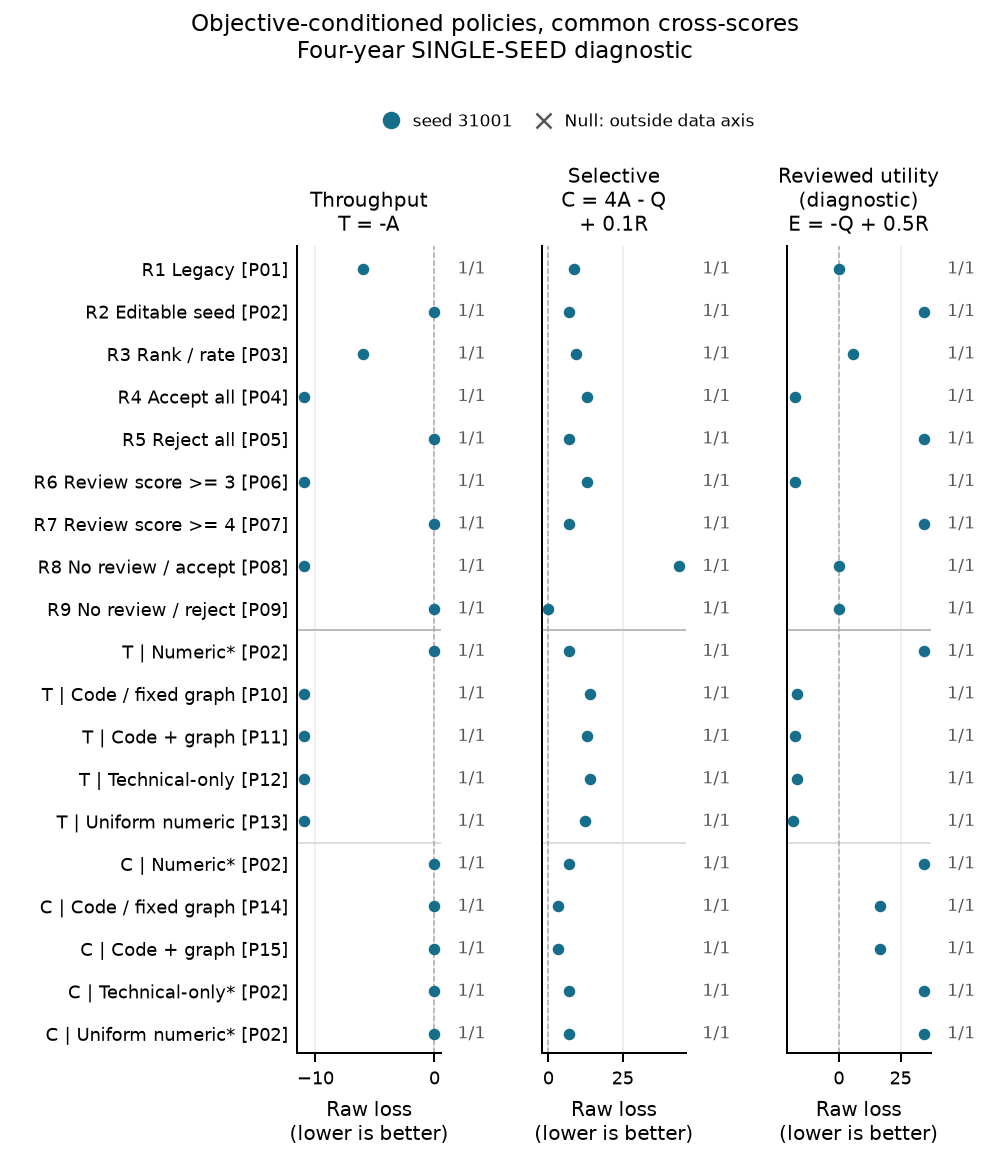
\includegraphics[width=\linewidth,height=.79\textheight,keepaspectratio]{figures/native-design-v2/cross-objective-4y.png}
\caption{\textbf{V2 separate four-year diagnostic.} One seed, no confidence
band or extra independent five-seed sample. Same labels/sharing/loss definitions
as the two-year plot. A repeated exact policy is not another observation.}
\label{fig:integrated-four-year}
\end{figure}

\FloatBarrier
\section{Fixed-record incentives versus dynamic policy optima}
For V2, freeze $N$ realized records, original reviewer means $ q_i $ (zero without
review) and review count $R$. If $ z_i\in\{0, 1\}$ only changes acceptance on those
records, then
\begin{align}
 T_{\min}^{\rm rec}&=-N,\\
 C_{\min}^{\rm rec}&=0.1R+\sum_i\min(0, 4-q_i),\\
 E_{\min}^{\rm rec}&=0.5R+\sum_i\min(0,-q_i).
\end{align}
Zero coefficients remain ties. For a full measured trajectory with $A>0$,
$C<0$ requires $Q/A>4+0.1R/A$. These elementary relations explain declared
incentives; they are not a new theorem or an optimal policy for the dynamic
world. Decisions affect later resubmissions, reviewer work, memory and resources.
The original reviews are endogenous rather than a fixed true-quality oracle.

The fixed-record projection contains 219 identities: 163 complete forwards and 56
unavailable entries. It does not execute 219 new worlds. Missing scores can make
a relaxation unavailable without invalidating a different measurable loss.
Neither this algebra nor AST/source inspection establishes equivalence on
unobserved inputs.

\section{Reproducibility, provenance and editorial scope}
\label{app:reproduction}
\subsection{Distinct execution identities}
The parameter study pins sourceZZPROTECTED 79ZZ and a simultaneous winner
sealZZPROTECTED 80ZZ. Structural V8 usesZZPROTECTED 81ZZ; free redesign
V12 usesZZPROTECTED 82ZZ; nested V13 usesZZPROTECTED 83ZZ.
The V10 method-path source isZZPROTECTED 84ZZ, and V11's native source
isZZPROTECTED 85ZZ. V2 usesZZPROTECTED 86ZZ. Full hashes, protocols and
original audit identities remain in machine-readable evidence records.
Historical reset worlds, coupled prefixes and source-equivalence bridges are
not relabeled a same-source matched experiment.

The original scientist alias isZZPROTECTED 87ZZ; the approved V2 local designer
alias isZZPROTECTED 88ZZ. Actual designer context is 40960 despite the
alias; the manifest/digest and model-load observations are retained. The upstream
revision and conversion command are unknown. Approved five HEAD-only registry
checks return advertised descriptor matches for three sampled local tensors
and two controls, with no body retrieval. They do not establish tensor contents,
all 986 descriptors, conversion provenance or fresh-machine reproducibility.

V2 uses 103107 CS 2016--2019 SciEvo records with pinned corpus/retriever binding.
The corpus is a literature-grounding substrate, not a license to redistribute
every underlying document or proof of scientific validity. Current public
model tags are not assumed equivalent to local retained weights.

\subsection{Audit and reconstruction tiers}
V2 closes with a matching normal terminal record, actual process exit 0 and
closed progress. Selection precedes first evaluation. Two read-only full audits
match byte-for-byte and verify 278 source blobs and 7038 raw files. A pinned
order-only adapter reconstructs equal-valued plan/selection mapping order lost
by sorted JSON. It preserves values, hashes, list chronology and original guards;
the unmodified frozen audit CLI is not claimed to pass. Replaying an auditor
does not create independent scientific evidence.

The exact retained closed-report archive supports numerical reconstruction:
120 statuses/ties and 90 evaluations rejoin, 462 T/C/E losses recompute from
measured $A/Q/R$ with zero residual, and 22 PNGs match the reviewed originals.
Exact auxiliary/scientist cost projections separately rebuild the full
supplement. This is not raw inference or independent replication. Paper-only
13-path subsets rebuild offline with cached tooling; rendered pages and text
match their reviewed variants, not necessarily binary PDF bytes. A cache-free
clean-machine build and fresh-model inference have not been established.

The repository exposes reproduction commands, compact JSON/CSV projections,
source-bound receipts and figure provenance. Large caches, reply databases,
corpus and model weights remain outside the publication subset. Complete
numerical projections include operational locators and are not certified
anonymous supplements. Author-name removal alone is not anonymity, rights
clearance or permission to upload. Human authors must review and accept
responsibility before an actual submission.

\subsection{What was deliberately not expanded into the scientific narrative}
Earlier local-author failures, copy controls, transport fixes and loop-retention
pilots are retained in the repository. They inform literal execution,
context-budget and completion checks. We do not count test-suite sizes or a
repaired editor protocol as a scientific discovery. S1's strong controls and
V1's eight-slot feedback pilot motivated V2 but are not pooled with its fresh
references. Numerical miniature/unit worlds verify implementations and do not
replace native-world results. Repeated UI screenshots are omitted in favor of
one actual evidence view.

These editorial choices remove duplication and weak evidence for broad claims,
not entire research tracks. This integrated manuscript restores the design,
gradient, structural, objective and UI arguments while keeping every retained
study's limitations. A longer paper is not new evidence or an automatic remedy
for the significance gap identified in the prior submission review.

\end{document}
